\documentclass[t,unknownkeysallowed,handout%
]{beamer}

%\includeonly{stream}
\mode<presentation>

\usetheme[
  outer/progressbar=none,
  color/block=fill,
  inner/sectionpage=simple
  ]
  {metropolis}


\usepackage[ngerman]{babel}
\usepackage{graphicx}
\usepackage{array}
\usepackage{amsmath}
\usepackage[official,right]{eurosym}
\usepackage{ifthen}
\usepackage{pgf}
\usepackage{alltt}
% \usepackage[scaled=.85]{luximono}
%\usefonttheme[onlymath]{serif}
\usepackage[ngerman]{datetime}
\usepackage{colortbl}
\usepackage{booktabs}
\usepackage{makecell}

\usepackage{listings}

%%%%%%%%%%%%%%%%%%%%%%%%%%%%%%% some macros %%%%%%%%%%%%%%%%%%%%%%%%%%%%%%%%%%
\definecolor{structure}{rgb}{0.1,0.1,0.7}
\definecolor{azureblue}{rgb}{0.0, 0.5, 1.0}
\definecolor{Gray}{gray}{0.85}

\newcommand{\settabs}{12\= 12\= 12\= 12\= 12\= 12\= 12\=
  123\= 123\= 123\= 123\= 123\= 123\= \kill}

\newcommand{\1}{\>}
\newcommand{\2}{\> \>}
\newcommand{\3}{\> \> \>}
\newcommand{\4}{\> \> \> \>}
\newcommand{\5}{\> \> \> \> \>}
\newcommand{\6}{\> \> \> \> \> \>}

\definecolor{darkgreen}{rgb}{0.0, 0.5, 0.0}
\newcommand{\prompt}[1]{{\color{darkgreen}#1}}
\newcommand{\pycomment}[1]{\color{darkgray}\textit{\# #1}}
\newcommand{\ccomment}[1]{\textrm{\textit{#1}}}

\definecolor{light-gray}{gray}{0.95}
\lstset{
	basicstyle=\scriptsize\ttfamily,
	numbers=left,
	language=python,
	frame=single,
	frameround=tttt,
	showstringspaces=false,
	backgroundcolor=\color{light-gray}
}

\newcommand{\code}[1]{\texttt{#1}}

\setbeamertemplate{frame numbering}{\insertpartnumber{}--\insertframenumber{}}
\setbeamertemplate{part page}{
\setcounter{framenumber}{0}
\begin{centering}
  {\usebeamerfont{part name}\usebeamercolor[fg]{part
  name}\partname~\insertromanpartnumber}
\vskip1em\par
\begin{beamercolorbox}[sep=8pt,center]{part title}
  \usebeamerfont{part title}\insertpart\par
\end{beamercolorbox}
\end{centering}
}

\setbeamercolor{algo color}{fg=black,bg=structure.fg!15!white}%

\newenvironment{algo}{%
  \bgroup\small\ttfamily
%  \fontfamily{pfr}\fontseries{mc}\selectfont
    \hspace*{.5cm}%
  \begin{beamercolorbox}%
[sep=4pt,colsep*=5pt,shadow=false,rounded=false]{algo color}%
    \begin{minipage}{10cm}
    \begin{tabbing}%
    \settabs}
  {\end{tabbing}\end{minipage}\end{beamercolorbox}\egroup}%

\newenvironment{smallalgo}{%
  \bgroup\scriptsize\ttfamily
%  \fontfamily{pfr}\fontseries{mc}\selectfont
    \hspace*{.5cm}%
  \begin{beamercolorbox}%
[sep=4pt,colsep*=5pt,shadow=false,rounded=false]{algo color}%
    \begin{minipage}{10cm}
    \begin{tabbing}%
    \settabs}
  {\end{tabbing}\end{minipage}\end{beamercolorbox}\egroup}%

\newenvironment{sql}{%
  \bgroup\small\ttfamily
%  \fontfamily{pfr}\fontseries{mc}\selectfont
    \hspace*{.5cm}%
  \begin{beamercolorbox}%
[sep=4pt,colsep*=5pt,shadow=false,rounded=false]{algo color}%
    \begin{minipage}{10cm}
    \begin{tabbing}%
    \settabs}
  {\end{tabbing}\end{minipage}\end{beamercolorbox}\egroup}%

\newenvironment{python}{%
  \bgroup\footnotesize\ttfamily
%  \fontfamily{pfr}\fontseries{mc}\selectfont
    \hspace*{.5cm}%
  \begin{beamercolorbox}%
[sep=4pt,colsep*=5pt,shadow=false,rounded=false]{algo color}%
    \begin{minipage}{10cm}
    \begin{tabbing}%
    \settabs}
  {\end{tabbing}\end{minipage}\end{beamercolorbox}\egroup}%

\setbeamercolor{wichtig}{fg=blue,bg=structure.fg!20!white}

\newenvironment{notebox}{%
\begin{beamercolorbox}[sep=4pt,colsep*=5pt,shadow=false,rounded=false]{wichtig}}%
{\end{beamercolorbox}}

\newcommand{\jcomment}[1]{\color{structure}#1}
\newcommand{\op}[1]{\texttt{\textbf{#1}}}
% \newcommand{\op}[1]{%
% \fontfamily{pfr}\selectfont\underline{\textbf{#1}}}

\newcommand{\hl}[1]{{\color{blue}{\textbf{#1}}}}

\newcommand{\dist}{\operatorname{dist}}

\AtBeginDocument{\selectlanguage{ngerman}}
\newdateformat{mydate}{\monthname[\THEMONTH] \THEYEAR}

\AtBeginDocument{\mydate}

\title{VL Data Science -- Grundlagen}
\subtitle{Sommersemester 2023}
\author[\copyright~Sattler]{Prof. Dr.-Ing. Kai-Uwe Sattler}
\institute[]{TU Ilmenau\\FG Datenbanken \& Informationssysteme}
\date{Letzte {\"A}nderung: April 2023}

\setbeamertemplate{frame footer}{Sattler | VL Data Science I | \today}
\setbeamertemplate{section in toc}[sections numbered]



%%%%%%%%%%%%%%%%%%%%%%%%%%%%%%%%%%%%%%%%%%%%%%%%%%%%%%%%%%%%%%%%%%%%%%%%%%%%%%

\begin{document}

\frame[plain]{\titlepage}

%%%%%%%%%%%%%%%%%%%%%%%%%%%%%%%%%%%%%%%%%%%%%%%%%%%%%%%%%%%%%%%%%%%%%%

\setcounter{part}{0}%

\begin{frame}

    \frametitle{Wer, Wann, Wo?}
  
    \begin{itemize}
      \item Dozent: Prof. Kai-Uwe Sattler
      \item Zielgruppe: Bachelor Informatik
    \end{itemize}

    \begin{columns}
      \begin{column}{0.3\textwidth}
          \begin{center}
           
\includegraphics[width=3cm]{fig1/qr-ds1.png}
           \end{center}
      \end{column}
      \begin{column}{0.7\textwidth}
    \begin{itemize}
    \item Übung: Eric Tröbs
      \begin{itemize}
      \item Diskussion und Lösung praktischer Data-Science-Aufgaben
      \end{itemize}
    \item Prüfung: mündlich
    \end{itemize}
  \end{column}
\end{columns}
\end{frame}
  
  %%%%%%%%%%%%%%%%%%%%%%%%%%%%%%%%%%%%%%%%%%%%%%%%%%%%%%%%%%%%%%%%%%%%%%
  
  \begin{frame}
  
    \frametitle{Voraussetzungen \& Ablauf}
  
  \hl{Voraussetzungen}
  \begin{itemize}
  \item Vorlesung: Datenbanksysteme (Bachelor)
  \item Grundkenntnisse: Statistik, SQL, Python(?) \dots
  \end{itemize}


  \hl{Ablauf}
  \begin{itemize}
    \item "`hybride"' Vorlesung: Präsenz + Flipped Classroom für ausgewählte Teile
    \item Übungen mit praktischen (Haus-)Aufgaben (Jupyter, Einreichung über Moodle)
    \item Miniprojekt
    \end{itemize}
  
  \end{frame}
  
  %%%%%%%%%%%%%%%%%%%%%%%%%%%%%%%%%%%%%%%%%%%%%%%%%%%%%%%%%%%%%%%%%%%%%%
  
  \begin{frame}
  
    \frametitle{Lernziele}
  
  \begin{itemize}
  \item Überblick über \hl{Grundlagen und Verfahren} von Data Science
  \item Fähigkeit 
  \begin{itemize}
  \item zum grundlegenden Umgang mit Daten ("`Data Literacy"')
  \item zur Auswahl, Bewertung und Einsatz konkreter Verfahren für
    gegebene Anwendung 
  \end{itemize}
  \item Kompetenzen in der \hl{praktischen Arbeit} mit Data-Science-Themen 
\end{itemize}
  
  \end{frame}

%%%%%%%%%%%%%%%%%%%%%%%%%%%%%%%%%%%%%%%%%%%%%%%%%%%%%%%%%%%%%%%%%%%%%%
  
  \begin{frame}
    \frametitle{Überblick}
  
    \begin{enumerate}
    \item<1-> Einführung: Was ist Data Science?
    \item<2-> Datenanalyse: Daten, Prozess, Aufgaben
    \item<3-> Werkzeuge zur Datananalyse: SQL, Python, Jupyter
    \item<4-> Datenbeschaffung, -vorbereitung und -bereinigung
    \item<5-> Datenvisualisierung
    \item<6-> Data Warehousing und OLAP
    \item<7-> Ausgewählte Analyseverfahren: Regression, Klassifikation, Clustering
    \item<8-> Analyse von Graphen
    \item<9-> Textanalyse
   \end{enumerate}
  
  \end{frame}
  
  %%%%%%%%%%%%%%%%%%%%%%%%%%%%%%%%%%%%%%%%%%%%%%%%%%%%%%%%%%%%%%%%%%%%%%
  
  
  \begin{frame}
    \frametitle{Weitere Literatur}
  
    \begin{thebibliography}{Ester, 2000}
     \bibitem[VanderPlas, 2018]{VanderPlan, 2018}
     J. VanderPlas.
     \newblock {\em Data Science mit Python}. 
     \newblock mitp-Verlag, 2018.  
     \bibitem[Herbold, 2022]{Herbold, 2022}
     S. Herbold.
     \newblock {\em Data Science Crashkurs}. 
     \newblock dpunkt-Verlag, 2022.    
     \bibitem[Saake, 2018]{Saake, 2018}
     G. Saake, K. Sattler, A. Heuer.
     \newblock{\em Datenbanken --- Konzepte und Sprachen}
     \newblock 6. Auflage, mitp-Verlag, 2018.
     \bibitem[Köppen, 2014]{Köppen, 2014} 
     V. Köppen, G. Saake, K. Sattler.
     \newblock {\em Data Warehouse Technologien}. 
     \newblock 2. Auflage, mitp-Verlag, 2014.    

  %\bibitem[Zhao, 2013]{Zhao, 2013}
  %  Y. Zhao.
  %  \newblock {\em R and Data Mining: Examples and Case Studies}. 
  %  \newblock Elsevier, 2013.  
  %  \newblock \url{http://www.rdatamining.com}.
  \end{thebibliography}
  
  \end{frame}
  

%%%%%%%%%%%%%%%%%%%%%%%%%%%%%%%%%%%%%%%%%%%%%%%%%%%%%%%%%%%%%%%%%%%%%%

\part{Einführung: Was ist Data Science?}

\frame[plain,c]{\partpage}

\frame{
  \frametitle{Überblick}

 \tableofcontents[pausesections,hidesubsections]

}

% Kapitel: Einleitung


\section{Motivation}

%---------------------------------------------------------------------

\begin{frame}
\frametitle{Überblick}

% Abbildung
\begin{center}
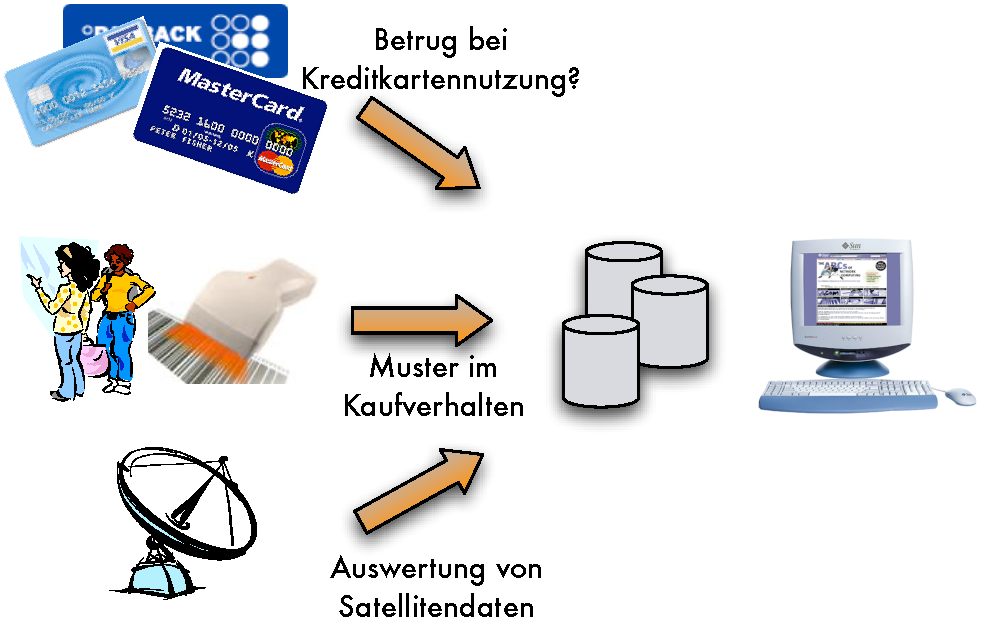
\includegraphics[scale=.5]{fig1/motivation.pdf}
\end{center}


Analyse muss durch "`Vorarbeit"' des Systems unterstützt werden

\end{frame}

%---------------------------------------------------------------------

\begin{frame}
\frametitle{Kommerzieller Bereich}

\begin{minipage}[c]{7cm}
\begin{itemize}
\item Erfassung und Speicherung großer Datenmengen
\begin{itemize}
\item Artikeldaten, Lagerbestände, Warenbewegungen, Lieferantendaten
\item Kaufvorgänge, Kreditkartentransaktionen
\item Nutzerdaten, Kundenbefragungen
\end{itemize}
\item Datenauswertung mit dem Ziel
\begin{itemize}
\item Optimierung der Prozesse
\item Verbesserung des Service
\item Senkung der Kosten
\end{itemize}
\end{itemize}
\end{minipage}\quad
\begin{minipage}[c]{3cm}
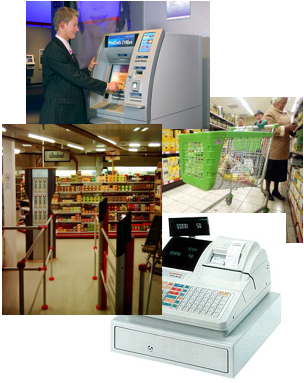
\includegraphics[scale=.3]{fig1/kommerz-anwendung.png}
\end{minipage}

\end{frame}

%---------------------------------------------------------------------

\begin{frame}
\frametitle{Wissenschaftlicher Bereich}

\begin{minipage}[c]{7cm}
\begin{itemize}
\item automatisierte Beobachtung und Erfassung
\begin{itemize}
\item Himmelsteleskope
\item Simulationsmodelle (Wetter, Erdbeben, \dots)
\item Microarrays in der Genforschung
\end{itemize}
\item Produktion riesiger Datenbestände (GB/Stunde)
\begin{itemize}
\item manuelle Aufbereitung und Auswertung kaum mäglich
\end{itemize}
\item Ziele einer Analyse
\begin{itemize}
\item Klassifikation / Segmentierung der Daten
\item Erstellung von Hypothesen
\end{itemize}
\end{itemize}
\end{minipage}\quad
\begin{minipage}[c]{3cm}
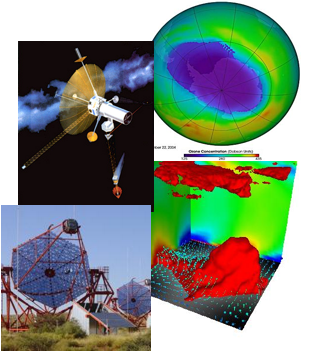
\includegraphics[scale=.3]{fig1/wiss-anwendung.png}
\end{minipage}

\end{frame}

%---------------------------------------------------------------------


\begin{frame}
\frametitle{Analyse großer Datenbestände}

\begin{itemize}
\item Analyse von Daten in Datenbanken (GB \dots PB)
\item "`versteckte"' Informationen: Muster, Abhängigkeiten, \dots
\begin{itemize}
\item manuell nicht identifizierbar
\item aufgrund des Datenvolumens oft überhaupt keine Analyse möglich
\end{itemize}
\end{itemize}


% Abbildung
\begin{center}
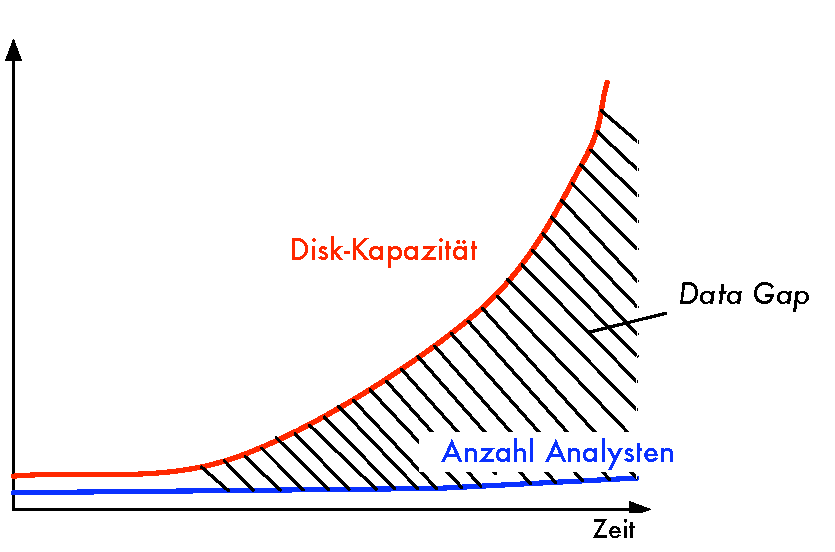
\includegraphics[scale=.45]{fig1/data-gap.pdf}
\end{center}

\end{frame}

%---------------------------------------------------------------------

\begin{frame}
\frametitle{Big Data Analytics}

\begin{itemize}
\item Analyse sehr großer Datenbestände:
\begin{itemize}
\item Fraud Detection bei Kreditkartenunternehmen und
  Finanztransaktionen (Bsp.: Mastercard -- jährlich 8 Mrd. \$ Schaden)
\item  Behavioral Analysis in Suchmaschinen und Sozialen Netzen
\item Genom-und Pharmaforschung
\item \dots
\end{itemize}
\item "`Enabler"': Verfügbarkeit von Speicherkapazität
  (Festplattenproduktion, Cloud), Berechnungskapazität (Serverfarmen), Daten
\item V3: \hl{Volume} (TB $\leadsto$ ZB), \hl{Velocity} (Batch Processing
  $\leadsto$ Realtime/Stream Processing), \hl{Variety} (strukturierte
  $\leadsto$ (semi-)strukturierte Daten)
\end{itemize}

\end{frame}

%---------------------------------------------------------------------

%\begin{frame}
%\frametitle{Data Analytics / ML im Gartner Hype Cycle}
%
%\begin{center}
%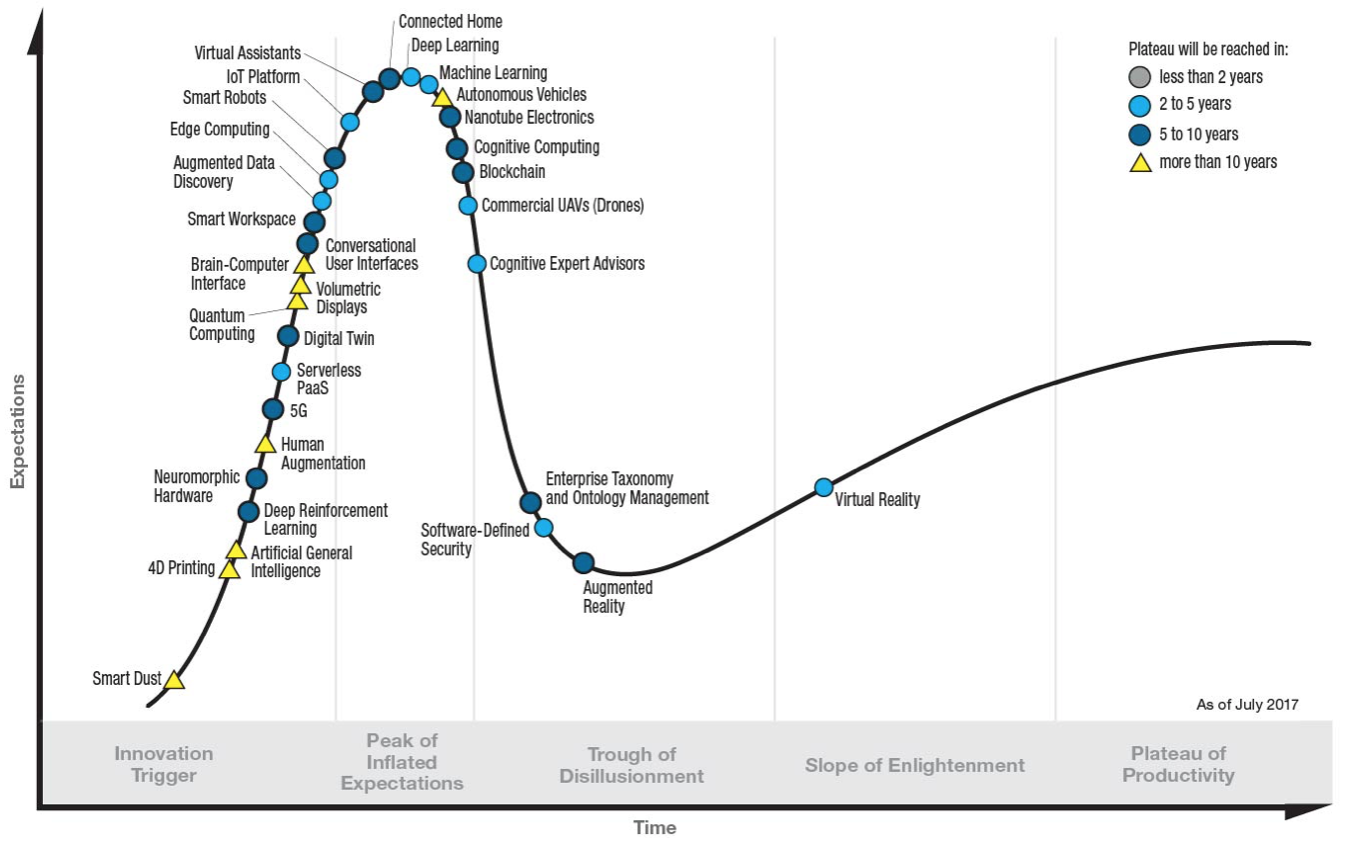
\includegraphics[scale=.45]{fig1/gartner_hype_cycle_2017.png}
%\end{center}
%
%\footnotesize{Quelle: Gartner}
%\end{frame}

%%%%%%%%%%%%%%%%%%%%%%%%%%%%%%%%%%%%%%%%%%%%%%%%%%%%%%%%%%%%%%%%%%%%%%

\section{Begriff Data Science}


\begin{frame}
  \frametitle{Data Science}

  \begin{block}{Data Science}
  interdisziplinäres Wissenschaftsfeld, welches wissenschaftlich fundierte Methoden, Prozesse, Algorithmen und Systeme zur Extraktion von Erkenntnissen, Mustern und Schlüssen sowohl aus strukturierten als auch unstrukturierten Daten ermöglicht (Wikipedia)
  \end{block}

  \begin{itemize}
  \item The key word in "`Data Science"' is not Data, it is Science (Jeff Lesk 2013 @ \url{https://simplystatistics.org/})
  \begin{itemize}
  \item Data Mining als Teilschritt -- Data Science als Prozess
  \item Data Mining/ML-Methoden können in verschiedenen Teilschritten zum Einsatz kommen
  \end{itemize}
  \end{itemize}
  \end{frame}

  %---------------------------------------------------------------------

  \begin{frame}
    \frametitle{Data Science: Einflussgebiete}

    \begin{center}
      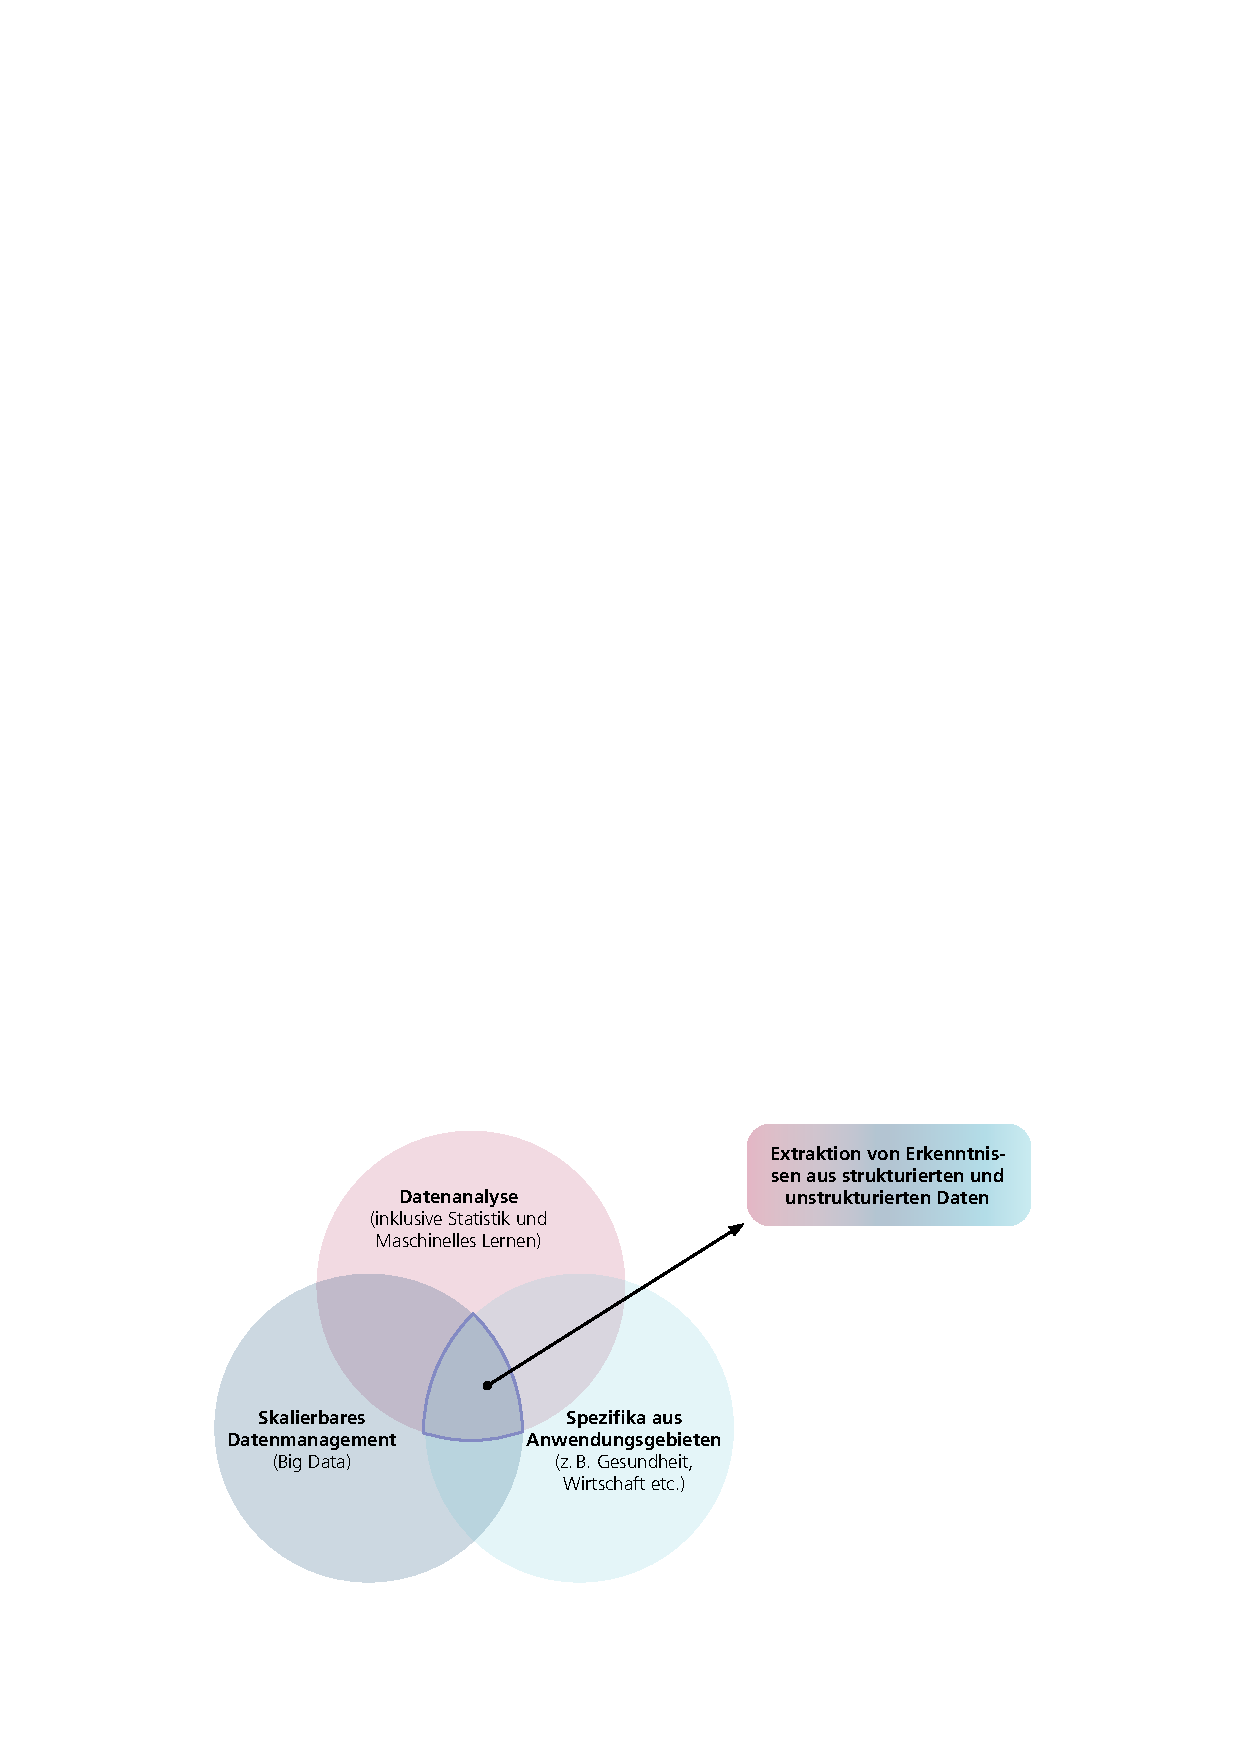
\includegraphics[scale=.7]{fig1/ds-einfluss.pdf}
      \end{center}

  \tiny{Keim, Sattler: Von Daten zu KI --Intelligentes Datenmanagement als Basis für Data Science und den Einsatz Lernender Systeme, Whitepaper Plattform Lernende Systeme, München 2020}
  \end{frame}

  %---------------------------------------------------------------------

\section{Anwendungsbeispiele}

\begin{frame}
  \frametitle{Anwendungsbeispiele}

  \begin{itemize}
\item \hl{Betrugsaufklärung}: Betrugserkennung u.a. bei Banken und Kreditkartenunternehmen durch Analyse der Transaktionsdaten
\item \hl{Medizin}: Systeme zur Unterstützung von Medizinern bei der Diagnose etwa durch Analyse von Röntgenbildern oder Hautbildern zur Krebserkennung
\item \hl{Physik}: Forschung im Bereich der Hochenergiephysik wie das IceCube-Projekt zum Nachweis von Neutrino-Ereignissen oder Arbeiten am LHC des CERN zur Erforschung der Natur der Elementarteilchen und ihrer Wechselwirkungen

\end{itemize}
\end{frame}

%---------------------------------------------------------------------

\begin{frame}
  \frametitle{Anwendungsbeispiele /2}

  \begin{itemize}
    \item \hl{Autonomes Fahren}: zur Klassifikation und Erkennung von Verkehrssituationen anhand der Sensordaten
\item \hl{Sprachassistenten und Übersetzungsdienste}: Erkennung und Übersetzung natürlicher Sprache durch das Training mit großen Datenmengen
\item \hl{Vorausschauende Wartung}: Zustandsüberwachung und vorausschauende Wartung von Produktionsmitteln mit Hilfe von Sensordaten und ML
\item \hl{Werbemarkt}: Modellierung und Vorhersage von Nutzerverhalten

  \end{itemize}
  \end{frame}

%---------------------------------------------------------------------

\section{Datenschutz und Privacy}

\begin{frame}
  \frametitle{Data Privacy und Datenschutz}

 
\hl{Data Privacy} abgeleitet aus Grundgesetz und dem Recht auf informationelle Selbstbestimmung

\begin{block}{Recht auf informationelle Selbstbestimmung}
das Recht des Einzelnen, grundsätzlich selbst über die Preisgabe und Verwendung seiner personenbezogenen Daten zu bestimmen
\end{block}

\begin{itemize}
  \item kein Eingriff bei Verarbeitung von Daten, die \hl{keinen Personenbezug} aufweisen
  \item sonst: DSGVO -- \hl{Zweckbindungsgrundsatz}: 
  \begin{itemize}
    \item Daten dürfen grundsätzlich nur für den Zweck verwendet werden, für den sie zu Beginn erhoben wurden 
    \item  Einholung einer Einwilligung als Rechtsgrundlage einer Datenverarbeitung
  \end{itemize}
\end{itemize}
\end{frame}

  %---------------------------------------------------------------------

\begin{frame}
  \frametitle{Datenschutzaspekte: DSGVO}
  
  \begin{itemize}
  \item regelt die Verarbeitung personenbezogener Daten
  \item bindend für natürliche Personen (!), Unternehmen und Organisationen in der gesamten europäischen Union
  \item verschiedene Pflichten, u.a. Auskunfts- und Meldepflichten
  \item hohe Geldbußen bei Verstößen
  \end{itemize}
      
  \end{frame}
  
  
%---------------------------------------------------------------------

\begin{frame}
\frametitle{Datenschutzaspekte}

\begin{itemize}
\item Gefahren des Missbrauchs der Data-Mining-Techniken
\item z.B. wenn personenbezogene Daten ohne Kenntnis der
  betroffenen Person gesammelt und analysiert werden
\item Aspekt des Datenschutzes (Privacy) im Zusammenhang mit Data Mining
\item Beispiele
\begin{itemize}
\item Edward-Snowden-Affäre
\item Wahlkampfmanipulation: Cambridge Analytica
\item Überwachung: Palantir Technologies
\end{itemize}
\end{itemize}

\end{frame}

%---------------------------------------------------------------------

\begin{frame}
\frametitle{Datenschutzaspekte:  Aufdecken von Identitäten}

\begin{itemize}
\item Data Broker Report, FTC Mai 2014
\begin{itemize}
\item Beispiel Acxiom: umfassende Daten von über 700 Mill. Kunden weltweit,
bis zu 1.500 Datenpunkte pro Kunde!
\item Dienste: Marketing, Risikobewertung (Kreditwürdigkeit, Identitäts-/ Missbrauchserkennung), Personensuche
\item Datensammlung aus verschiedensten Quellen (inkl. Offline-Daten) ohne Wissen der Kunden, fehlende Transparenz
\item falsche Risikobewertung, Datenmissbrauch
\end{itemize}
\item Beispiel Target: Erkennung der Schwangerschaft einer Kundin anhand der gekauften Artikel
\item Predictive Policing, Bias
\end{itemize}
\end{frame}

%---------------------------------------------------------------------

\begin{frame}
  \frametitle{Datenschutzaspekte: Persönlichkeitsprofile}

\begin{itemize}
\item Persönlichkeitsprofile aus Facebook-Daten: OCEAN-Modell
\item Offenheit für Erfahrungen (Aufgeschlossenheit)
\item Gewissenhaftigkeit (Perfektionismus)
\item Geselligkeit
\item Verträglichkeit (Rücksichtnahme, Kooperationsbereitschaft, Empathie)
\item Verletzlichkeit
\end{itemize}

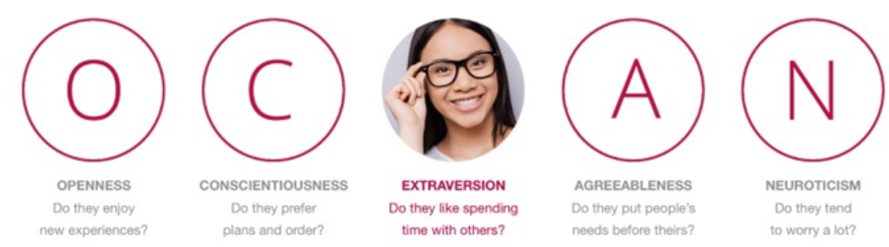
\includegraphics[scale=.7]{fig1/ocean.png}
\end{frame}

%---------------------------------------------------------------------

\begin{frame}
  \frametitle{Datenschutzaspekte: Persönlichkeitsprofile}


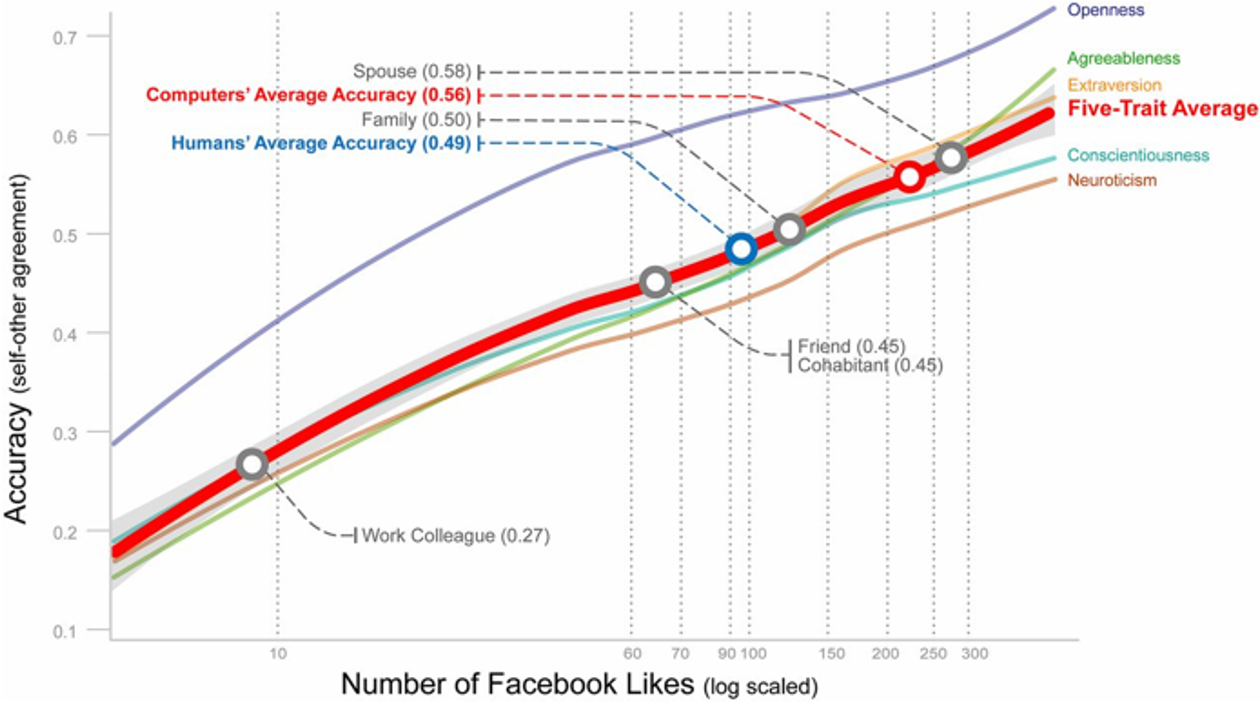
\includegraphics[scale=.5]{fig1/ocean-diagramm.png}

\footnotesize{Youyou, Kosinski, Stillwell Computer-based personality judgments are more accurate than those made by humans, PNAS 2015
}
\end{frame}

%---------------------------------------------------------------------

\begin{frame}
\frametitle{Zusammenfassung}

\begin{itemize}
\item Begriff \hl{Data Science}
\item \hl{Anwendungsbeispiele}
\begin{itemize}
\item Auswertung empirisch erfasster Daten
\item Analyse betriebswirtschaftlicher Daten, wissenschaftlicher
  Daten, Netzwerkdaten (Intrusion Detection, Web Mining, Web Log
  Mining), \dots
\item aber auch Textanalyse (Textklassifikation), Bildanalyse
  (Clustering von Bildern), \dots
\end{itemize}
\item \hl{Datenschutz}
\begin{itemize}
\item wichtiger Aspekt bei der Analyse personenbezogener Daten
\end{itemize}
\end{itemize}

\end{frame}

%---------------------------------------------------------------------

%%% Local Variables:
%%% mode: latex
%%% TeX-master: "main"
%%% End:


%%%%%%%%%%%%%%%%%%%%%%%%%%%%%%%%%%%%%%%%%%%%%%%%%%%%%%%%%%%%%%%%%%%%%%

\part{Datenanalyse: Daten, Prozess, Aufgaben}

\frame[plain,c]{\partpage}

\frame{
  \frametitle{Überblick}
  \tableofcontents[pausesections,hidesubsections,firstsection=5]

}


\section{Eigenschaften von Daten}


\begin{frame}
\frametitle{Strukturierte Daten}

\begin{itemize}
\item Menge von Datenobjekten
\item Objekte beschrieben durch ihre Eigenschaften (Attribute)
\item Attribut (Merkmal) vs. Attributwert (Ausprägung)
\begin{itemize}
\item ein Attribut $\longrightarrow$ verschiedene Attributwerte\\
z.B. Währung in \euro\ oder \$
\item verschiedene Attribute $\longrightarrow$ gleicher Attributwert\\
z.B. Kunden-Nr., Alter, Anzahl: \op{int}
\end{itemize}
\end{itemize}
\end{frame}

%---------------------------------------------------------------------

\begin{frame}
\frametitle{Attribute: Typen \& Eigenschaften}

\begin{itemize}
\item \hl{nominal}: Unterscheidung von Werten
\begin{itemize}
\item Bsp.: ID, PLZ, Geschlecht
\item Operationen: $=$, $\neq$
\end{itemize}
\item \hl{ordinal}: Festlegung einer Ordnung für Werte
\begin{itemize}
\item Bsp.: Zensur, Rang, Rating
\item Operationen: $=$, $\neq$, $<$, $>$
\end{itemize}
\item \hl{Intervall}: Differenz von Werten
\begin{itemize}
\item Bsp.: Datum, Zeit
\item Operationen: $=$, $\neq$, $<$, $>$, $+$, $-$
\end{itemize}
\item \hl{Ratio/Verhältnis}
\begin{itemize}
\item Bsp.: Menge, Anzahl, Länge
\item Operationen: $=$, $\neq$, $<$, $>$, $+$, $-$, $*$, $/$
\end{itemize}
\end{itemize}

\end{frame}

%---------------------------------------------------------------------

\begin{frame}
\frametitle{Diskrete vs. stetige Attribute}

\begin{itemize}
\item \hl{diskrete Attribute}
\begin{itemize}
\item endliche bzw. abzählbar unendliche Wertemenge
\item Datentyp: meist \op{integer}
\item Bsp.: Anzahl, Menge, PLZ, \dots
\end{itemize}
\item \hl{stetige bzw. kontinuierliche Attribute}
\begin{itemize}
\item reellwertiger Wertebereich
\item werden jedoch meist mit endlicher Anzahl von Stellen repräsentiert
\item Datentyp: \op{float}, \op{double}, \op{decimal}
\item Bsp.: Preis, Masse, Temperatur
\end{itemize}
\end{itemize}

\end{frame}

%---------------------------------------------------------------------


\begin{frame}
\frametitle{Satzorientierte Daten}

\begin{itemize}
\item Menge von Sätzen (Records) mit fester Attributmenge
\end{itemize}

{\small
\begin{tabular}{|c|c|c|c|c|}
\hline
\rowcolor{Gray} Kunden-ID & Schulden & Einkommen & Anstellungs- & Kredit- \\
\rowcolor{Gray}           &           &            & verhältnis   & würdigkeit \\
\hline\hline
1 & Hoch & Hoch & Selbständig & Schlecht \\
2 & Hoch & Hoch & Angestellt & Schlecht \\
3 & Hoch & Niedrig & Angestellt & Schlecht \\
4 & Niedrig & Niedrig & Angestellt & Gut \\
5 & Niedrig & Niedrig & Selbständig & Schlecht \\
6 & Niedrig & Hoch & Selbständig & Gut \\
7 & Niedrig & Hoch & Angestellt & Gut \\
\hline
\end{tabular}}

\end{frame}

%---------------------------------------------------------------------

\begin{frame}
\frametitle{Dokumentdaten}

\begin{itemize}
\item Dokumentrepräsentation als Vektor
\item Term (Schlüsselwort) repräsentiert Element im Vektor
\begin{itemize}
\item 0/1 für (Nicht-)Vorkommen
\item Häufigkeit des Vorkommens
\end{itemize}
\end{itemize}

\begin{center}
\begin{tabular}{|l|c|c|c|c|c|}
\hline
\rowcolor{Gray} & DBMS & KDD & Mining & Data & Web \\
\hline
\hline
Dokument \#1 & 3 & 2 & 0 & 1 & 0 \\
Dokument \#2 & 0 & 2 & 1 & 1 & 4 \\
Dokument \#3 & 0 & 0 & 2 & 4 & 3 \\
\hline
\end{tabular}
\end{center}

{\scriptsize
\begin{alltt}
\{"filter\_level":"medium","retweeted":false,\\
"{}in\_reply\_to\_screen\_name":"BeSassyChivette", \\
"possibly\_sensitive":false,"truncated":false,"lang":"{}en", \\
"id":553686454720032768,"timestamp\_ms":"1420844112459",\\
"created\_at":"Fri Jan 09 22:55:12 +0000 2015", \\
"text":"@BeSassyChivette gorgeous as usual", ... \}
\end{alltt}
}

\end{frame}

%---------------------------------------------------------------------

\begin{frame}
\frametitle{Transaktionsdaten}

\begin{itemize}
\item spezielle Form satzorientierter Daten
\item Datensatz entspricht Transaktion aus Transaktions-ID und Menge von Elementen (Items)
\end{itemize}

\begin{center}
\begin{tabular}{|c|l|}
\hline
\rowcolor{Gray} Transaktions-ID & Items \\
\hline
\hline
1 & Milch, Butter \\
2 & Milch, Honig, Butter \\
3 & Milch, Brot, Butter \\
4 & Milch, Brot, Honig \\
\hline
\end{tabular}
\end{center}


\end{frame}

%---------------------------------------------------------------------

\begin{frame}
\frametitle{Graphdaten}

\begin{itemize}
\item Graphstruktur, z.B. Web-Dokumente mit HTML-Links, soziale Netze, \dots
\end{itemize}

%\vspace*{-.5cm}
\begin{center}
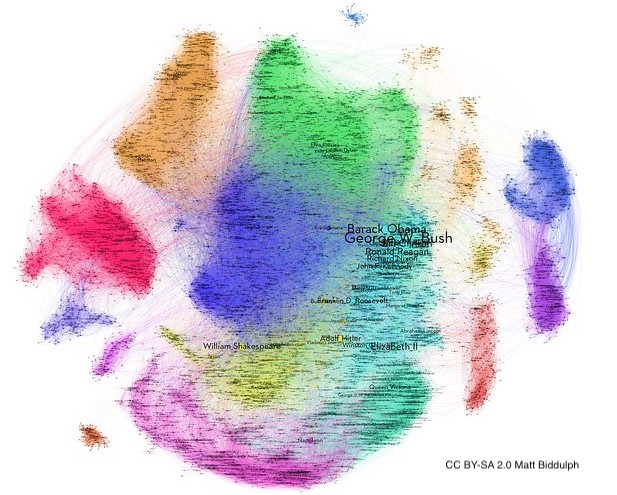
\includegraphics[scale=.35]{fig2/social-graph.jpg}
%{\tiny CC BY-SA 2.0 Matt Biddulph}
\end{center}
\end{frame}

%---------------------------------------------------------------------

\begin{frame}[fragile]
\frametitle{Ordnungsbasierte Daten}

\begin{itemize}
\item geordnete Folge von Elementen, z.B. Alarmmeldungen, Weblogs, Gensequenzen, spatio-temporale Daten
\end{itemize}

{\scriptsize
\begin{verbatim}
194.145.89.65 - - [19/Oct/2015:14:57:21 +0200] "GET ... HTTP/1.0"
194.145.89.65 - - [19/Oct/2015:14:57:21 +0200] "GET ... HTTP/1.0"
195.36.75.26 - - [19/Oct/2015:14:58:54 +0200] "GET ... HTTP/1.0"
195.37.152.250 - - [19/Oct/2015:15:02:55 +0200] "GET ... HTTP/1.1"
195.37.152.250 - - [19/Oct/2015:15:02:55 +0200] "GET ... HTTP/1.1"
193.51.91.2 - - [19/Oct/2015:15:06:20 +0200] "GET ... HTTP/1.0"
65.54.188.64 - - [19/Oct/2015:15:07:13 +0200] "GET ... HTTP/1.0"
84.168.66.17 - - [19/Oct/2015:15:12:02 +0200] "GET ... HTTP/1.1"
84.168.66.17 - - [19/Oct/2015:15:12:08 +0200] "GET ... HTTP/1.1"
68.142.251.148 - - [19/Oct/2015:15:22:14 +0200] "GET ... HTTP/1.0"
68.142.250.20 - - [19/Oct/2015:15:22:14 +0200] "GET ... HTTP/1.0"
\end{verbatim}
}

{%\scriptsize
\begin{verbatim}
ACAAGATGCCATTGTCCCCCGGCCTCCTGCTGCTGCTGCTCTCCGGGG
\end{verbatim}
}

\end{frame}

%---------------------------------------------------------------------

\section{Der Data-Science-Prozess}

\begin{frame}[c]
\frametitle{Data-Science-Prozess: Überblick}

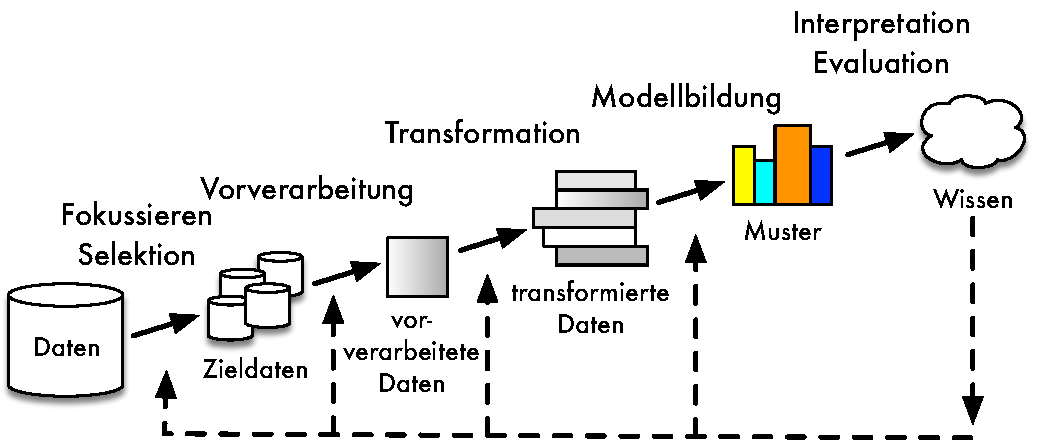
\includegraphics[scale=.6]{fig1/kdd-prozess.pdf}

\end{frame}

%---------------------------------------------------------------------

\begin{frame}
\frametitle{Prozess: Überblick /2}

\begin{itemize}
\item iterativer Prozess
\begin{itemize}
\item Selektion: Auswahl von Daten einer Datenbasis
\item Vorverarbeitung: Störungen wie Datenfehler oder
  Unvollständigkeit suchen und entfernen (entfällt beim Data Warehousing)
\item Transformation: Quantität verringern
\begin{itemize}
\item Attribute ohne oder mit geringem Vorkommen in der Datenbasis entfernen
\item in geeignete Analyseform umformen
\end{itemize}
\item Modellbildung: Aufgabenspezifikation bestimmt das Verfahren (statistische Verfahren, Data Mining, Machine Learning)
\item Interpretation und Verifikation
\end{itemize}
\end{itemize}


\end{frame}

%---------------------------------------------------------------------

\begin{frame}
\frametitle{Prozess: Fokussieren /Selektion}

\begin{itemize}
\item Auswahl der für die Analyseaufgabe notwendigen und relevanten Daten
\item ggf. Kampagne zur Datenerfassung notwendig
\item Beachtung der Datenqualität/-herkunft $\leadsto$ Vertrauenswürdigkeit, Grundprinzipien der Statistik
\item Vermeidung von Bias durch
\begin{itemize}
\item kognitive Verzerrungen (\url{https://de.wikipedia.org/wiki/Liste_kognitiver_Verzerrungen})
\item unvollständige Daten
\end{itemize}
\item Arbeit auf Dateien vs. ,,In-Database''-Analyse
\end{itemize}

\end{frame}

%---------------------------------------------------------------------

\begin{frame}
\frametitle{Prozess: Vorverarbeitung}

\begin{itemize}
\item Integration von Daten aus unterschiedlichen Quellen
\begin{itemize}
\item einfache Übersetzungen  von Attributnamen, z.B.\\
 \texttt{KNr} $\longrightarrow$ \texttt{KundenSchl}
\item Nutzen von Anwendungswissen um ähnliche Daten zusammenzufassen (z.B.
regionale Zuordnung von Postleitzahlen)
\end{itemize}
\item Konsistenzprüfung
\begin{itemize}
\item Test anwendungsspezifischer Konsistenzbedingungen
\item Bereinigung von Inkonsistenzen
\end{itemize}
\item Vervollständigung
\begin{itemize}
\item Ersetzen von unbekannten Attributwerten durch Defaults
\item Verteilung der Attributwerte soll i.A. erhalten bleiben!
\end{itemize}
\end{itemize}

\end{frame}

%---------------------------------------------------------------------

\begin{frame}
\frametitle{Prozess: Vorverarbeitung /2}

\begin{itemize}
\item Vorverarbeitung ist häufig einer der aufwendigsten Schritte -- bis zu 80\% des Gesamtaufwandes
\item wird häufig im Rahmen von Data-Warehouse-Systemen
durchgeführt
\end{itemize}

\begin{notebox}
\hl{Data Warehouse} :=
\begin{itemize}
\item \hl{dauerhafte}
\item \hl{integrierte} Sammlung von Daten
\item aus \hl{unterschiedlichen} Quellen
\item zum \hl{Zweck der Analyse} bzw. Entscheidungsunterstützung
\end{itemize}
\end{notebox}

\end{frame}

%---------------------------------------------------------------------

\begin{frame}
\frametitle{Data Warehousing: Prozess}

\begin{center}
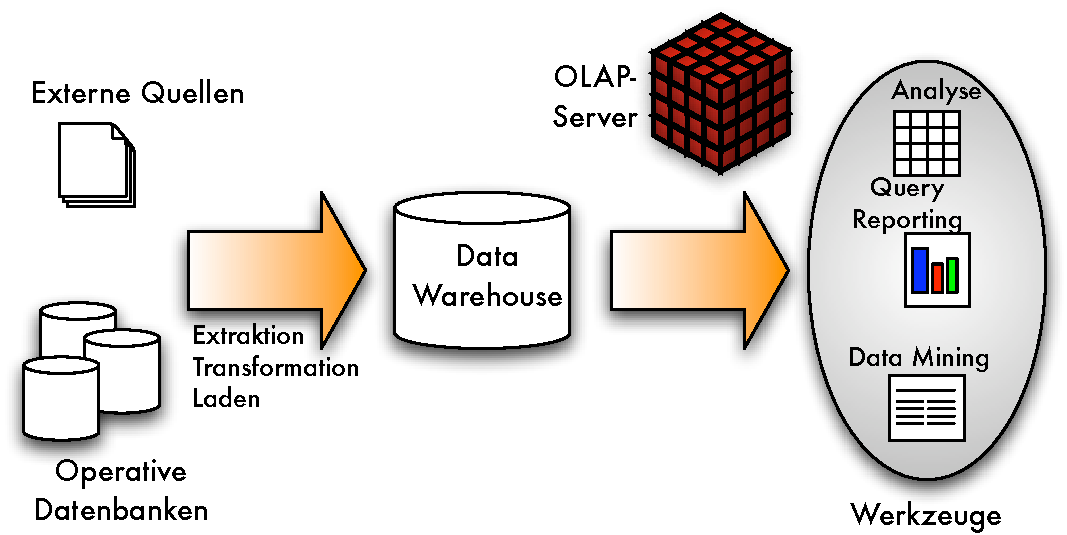
\includegraphics[scale=.6]{fig1/data-warehousing.pdf}
\end{center}

\end{frame}

%---------------------------------------------------------------------

\begin{frame}
\frametitle{Data Warehousing: Datenmodell}

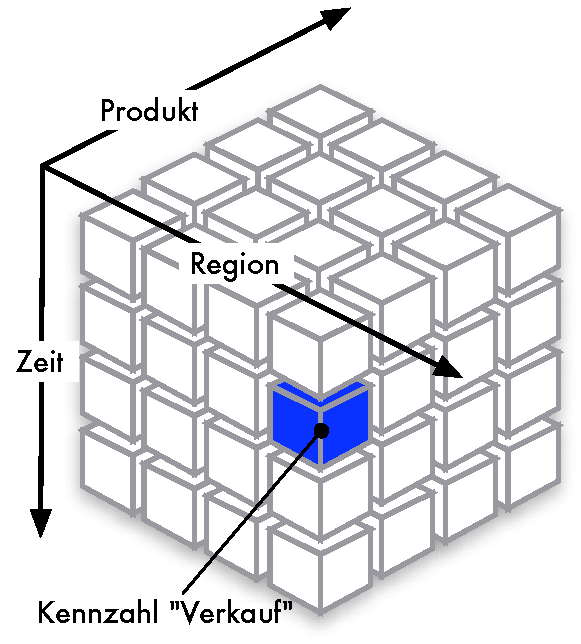
\includegraphics[scale=.4]{fig1/cube.pdf}\quad
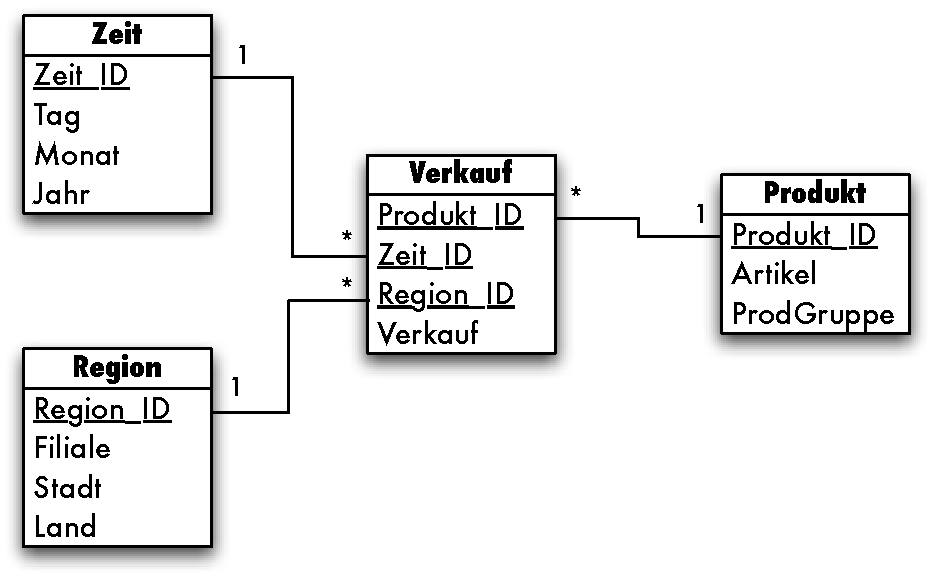
\includegraphics[scale=.4]{fig1/starschema.pdf}

\end{frame}

%---------------------------------------------------------------------

\begin{frame}
\frametitle{Prozess: Transformieren}

\begin{itemize}
\item Diskretisierung numerischer Attribute
\begin{itemize}
\item unabhängig von der Analyseaufgabe
z.B. Aufteilung des Wertebereichs in Intervalle gleicher Länge
\item abhängig von der Analyseaufgabe
z.B. Aufteilung in Intervalle so, dass der Informationsgewinn in Bezug auf die
Klassenzugehörigkeit maximiert wird
\end{itemize}

\item Erzeugen abgeleiteter Attribute / Feature-Extraktion
\begin{itemize}
\item durch Aggregation über Mengen von Datensätzen
z.B. von einzelnen Verkäufen zu "`Tagesumsatz, Wochenumsatz, Monatsumsatz"'
\item durch Verknüpfung mehrerer Attribute
z.B. Umsatzänderung = Umsatz 2018 - Umsatz 2017
\end{itemize}
\end{itemize}

\end{frame}

%---------------------------------------------------------------------

\begin{frame}
\frametitle{Prozess: Transformieren /2}

\begin{itemize}
\item Attribut-Selektion
\begin{itemize}
\item manuell:
\begin{itemize}
\item wenn Anwendungswissen über die Bedeutung der Attribute und über die
gegebene Datenanalyseaufgabe bekannt ist
\end{itemize}
\item automatisch:
\begin{itemize}
\item Bottom-Up (ausgehend von der leeren Menge jeweils ein Attribut
hinzufügen)
\item Top-Down (ausgehend von der Gesamtmenge der Attribute jeweils
  ein Attribut entfernen) z.B. so, dass die Diskriminierung der
  Klassen optimiert wird
\end{itemize}
\end{itemize}
\item Problem
\begin{itemize}
\item zu viele Attribute führen zu Ineffizienz und evtl. Ineffektivität
  des Data Mining
\item manche Transformationen können durch OLAP-Systeme realisiert
  werden
\end{itemize}
\end{itemize}

\end{frame}

%---------------------------------------------------------------------
\begin{frame}
  \frametitle{Prozess: Modellbildung}

  \begin{itemize}
    \item \hl{Ziel:} Ableitung eines Modells der Daten (=\hl{Abstraktion}) zur
    \begin{itemize}
      \item Beschreibung (für Aggregation/Generalisierung, Muster, Anomalieerkennung)
      \item Vorhersage
    \end{itemize}
        \item Methoden der klassischen Statistik: deskriptive, prädiktive und Inferenzstatistik
        \item \hl{Data Mining (statistische Verfahren)}
        \item Maschinelles Lernen, Deep Learning
      \end{itemize}

      \begin{center}
        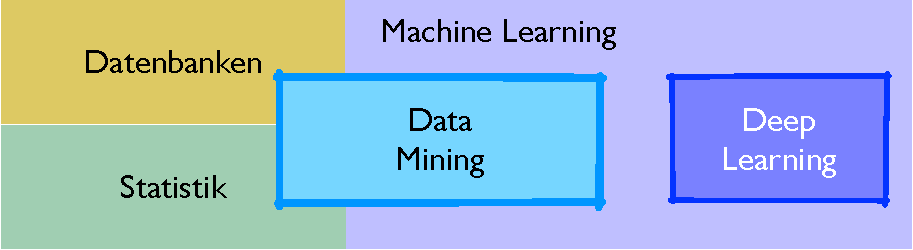
\includegraphics[scale=.6]{fig1/dm-vs-ml.pdf}
        \end{center}

\end{frame}
%---------------------------------------------------------------------

\begin{frame}
  \frametitle{Data Mining / Knowledge Discovery in Databases}

  Fayyad, Piatetsky-Shapiro \& Smyth
  \begin{notebox}
  Knowledge Discovery in Databases (KDD) ist der Prozess der (semi-)
  automatischen Extraktion von Wissen aus Datenbanken, das
  \hl{gültig}, \hl{bisher unbekannt} und \hl{potenziell nützlich} ist.
  \end{notebox}

  \begin{itemize}
  \item Anmerkungen
  \begin{itemize}
  \item (semi-)automatisch: im Unterschied zur manuellen Analyse, aber
    mit Nutzerinteraktion
  \item gültig: im statistischen Sinne
  \item bisher unbekannt: bisher nicht explizit vorhanden, kein
    "`Allgemeinwissen"'
  \item potenziell nützlich: für gegebene Anwendung
  \end{itemize}
  \end{itemize}

  \end{frame}



  %---------------------------------------------------------------------


\begin{frame}
  \frametitle{Data Mining}

  \begin{notebox}
  Data Mining ist die Anwendung effizienter Algorithmen, die die
    in der Datenbank enthaltenen Muster liefern
  \end{notebox}

  \begin{itemize}
  \item Prediktive Verfahren (Vorhersage):
  \begin{itemize}
  \item Nutzung von Merkmalen (Variablen) zur Vorhersage unbekannter
    oder zukünftiger Werte anderer Merkmale
  \item Beispiel: Klassifikation
  \end{itemize}
  \item Deskriptive Verfahren (Beschreibung):
  \begin{itemize}
  \item Extraktion von durch Menschen interpretierbare Muster, die die
    Daten beschreiben
  \item Beispiele: Assoziationsregeln, Clustering
  \end{itemize}
  \end{itemize}

  \end{frame}

  %---------------------------------------------------------------------


\begin{frame}
\frametitle{Prozess: Evaluation}

\begin{itemize}
\item Präsentation der gefundenen Muster: häufig durch entsprechende
  Visualisierungen
\item falls schlechte Bewertung (durch Benutzer): erneutes Data Mining mit
\begin{itemize}
\item anderen Parametern, anderem Verfahren, anderen Daten
\end{itemize}
\item falls gute Bewertung (durch Benutzer)
\begin{itemize}
\item Integration des gefundenen Wissens in die Wissensbasis
\item Nutzung des neuen Wissens für zukünftige KDD-Prozesse
\end{itemize}
\end{itemize}

\end{frame}

%---------------------------------------------------------------------

\begin{frame}
\frametitle{Prozess: Evaluation /2}

\begin{itemize}
\item Bewertung der gefundenen Muster
\begin{itemize}
\item Vorhersagekraft der Muster
\begin{itemize}
\item Verwendete Daten sind Stichprobe aus der Grundgesamtheit aller Daten.
\item Wie gut lassen sich die in diesen "`Trainingsdaten"' gefundenen
  Muster auf zukünftige Daten verallgemeinern?
\item Vorhersagekraft wächst mit Größe und Repräsentativität der Stichprobe.
\end{itemize}
\item Interessantheit der Muster
\begin{itemize}
\item Muster schon bekannt?
\item Muster überraschend?
\item Muster für viele Fälle anwendbar?
\end{itemize}
\end{itemize}
\end{itemize}

\end{frame}

%---------------------------------------------------------------------

\begin{frame}
  \frametitle{Data-Science-Stack}

  \begin{center}
    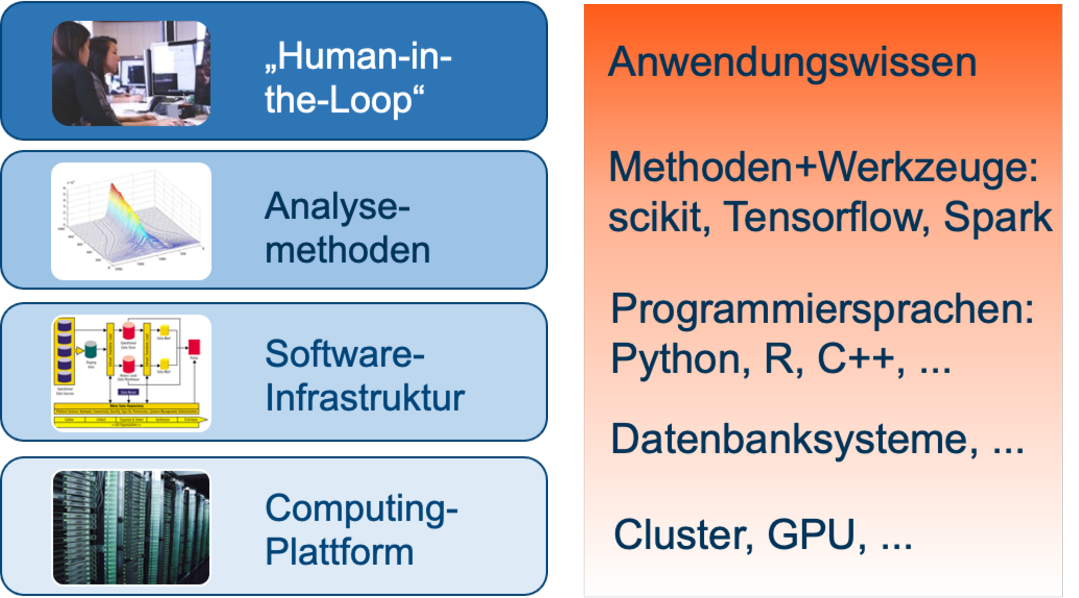
\includegraphics[scale=.6]{fig1/ds-stack.pdf}
    \end{center}

\end{frame}

%%%%%%%%%%%%%%%%%%%%%%%%%%%%%%%%%%%%%%%%%%%%%%%%%%%%%%%%%%%%%%%%%%%%%%

\section{Data-Science-Aufgaben}


\begin{frame}
  \frametitle{Regression}

\end{frame}

%---------------------------------------------------------------------

\begin{frame}
\frametitle{Klassifikation: Beispiel}


\begin{itemize}
\item  Zuordnung von Objekten zu verschiedenen vorgegebenen Klassen,
  d.h. Vorhersage von Merkmalen (Klassenzuordnung) anhand anderer
  Merkmale
    \item Ableitung des \hl{Klassifikationsmodells} aus einer Trainingsmenge
% \item Beispiel: Kundenklassifikation bzgl. Schadensrisiko
%   (Kreditausfall)
\end{itemize}

\begin{center}
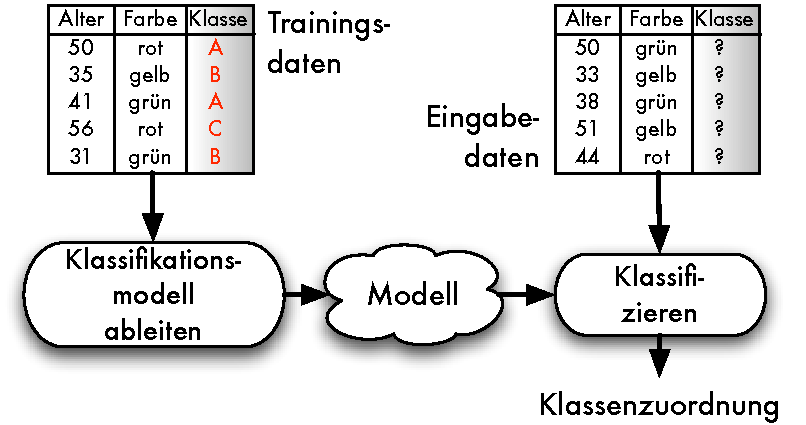
\includegraphics[scale=.6]{fig1/klassifikation-prinzip.pdf}
\end{center}

\end{frame}

%---------------------------------------------------------------------

\begin{frame}
\frametitle{Klassifikation: Beispiel /2}

{\tiny\begin{tabular}{|c|c|c|c|c|}
  \rowcolor{Gray}\hline
Kunden-ID & Schulden & Einkommen & Anstellungs- & Kredit- \\
\rowcolor{Gray}           &           &            & verhältnis   & würdigkeit \\
\hline\hline
1 & Hoch & Hoch & Selbständig & Schlecht \\
2 & Hoch & Hoch & Angestellt & Schlecht \\
3 & Hoch & Niedrig & Angestellt & Schlecht \\
4 & Niedrig & Niedrig & Angestellt & Gut \\
5 & Niedrig & Niedrig & Selbständig & Schlecht \\
6 & Niedrig & Hoch & Angestellt & Gut \\
7 & Niedrig & Hoch & Angestellt & Gut \\
\hline
\end{tabular}}

\raggedleft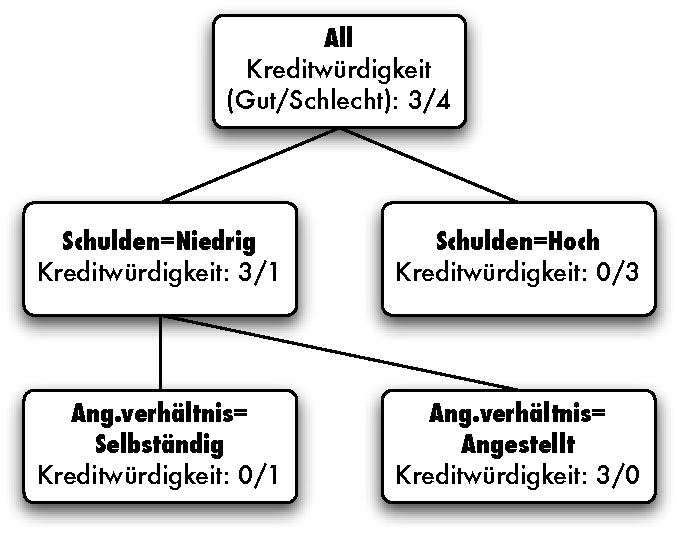
\includegraphics[scale=.5]{fig1/klassifikation.pdf}

\end{frame}

%---------------------------------------------------------------------

\begin{frame}
\frametitle{Assoziationsregeln: Beispiel}

\begin{itemize}
  \item Aufdeckung statistischer Zusammenhänge zwischen Variablen
  \item Modell: Assoziationsregeln oder "`Frequent Itemsets"'
\item Beispiel: Warenkorbanalyse
\end{itemize}

\begin{center}
\begin{tabular}{|c|l|}
\rowcolor{Gray}\hline
Transaktions-ID & Produkte \\
\hline
\hline
1 & Milch, Butter \\
2 & Milch, Honig, Butter \\
3 & Milch, Brot, Butter \\
4 & Milch, Brot, Honig \\
\hline
\end{tabular}
\end{center}
\end{frame}

%---------------------------------------------------------------------

\begin{frame}
\frametitle{Assoziationsregeln: Beispiel /2}

\begin{itemize}
\item Frequent Itemsets

{\small
\begin{center}
\begin{tabular}{|l|c|}
  \rowcolor{Gray}\hline
Produkte & Support \\
\hline
\hline
\{ Milch \} & 4 \\
\hline
\{ Butter \}, & 3 \\
\{ Milch, Butter \} & \\
\hline
\{ Honig \}, \{ Brot \}  & 2 \\
\{ Honig, Milch \},
\{ Brot, Milch \}  & \\
\hline
\end{tabular}\end{center}}

\item Ableitung von Regeln:\\
\fbox{\hl{Wenn ein Kunde Milch kauft, dann kauft er auch Butter.}}
\begin{itemize}
\item Unterstützung (Support): hier 3
\item Konfidenz: hier 75\%
\end{itemize}
\end{itemize}

\end{frame}

%---------------------------------------------------------------------

\begin{frame}[c]
\frametitle{Clustering: Beispiel}

\begin{minipage}[c]{5.5cm}
\begin{itemize}
\item Einordnung ähnlicher Objekte in neu gebildete Gruppen, so dass
\begin{enumerate}
\item Ähnlichkeit \hl{innerhalb} einer Gruppe möglichst \hl{groß},
\item Ähnlichkeit \hl{zwischen} Gruppen möglichst \hl{gering}
\end{enumerate}
\end{itemize}
\end{minipage}\quad
\begin{minipage}[c]{4cm}
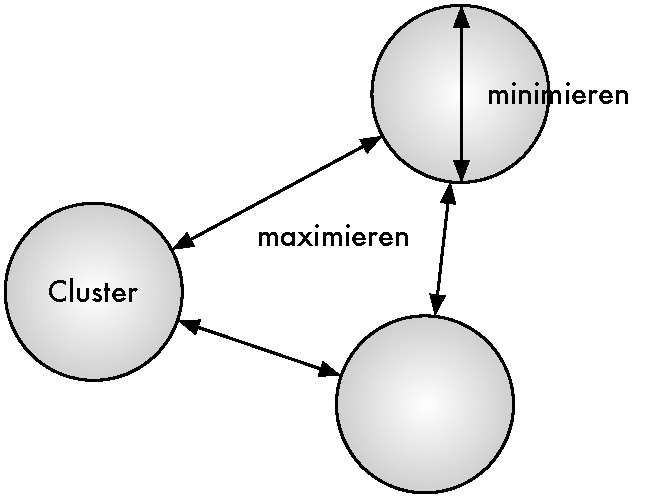
\includegraphics[scale=.5]{fig1/cluster.pdf}
\end{minipage}

\end{frame}

%---------------------------------------------------------------------

\begin{frame}[c]
\frametitle{Clustering: Beispiel /2}

\begin{minipage}[c]{3.5cm}
{\small\begin{tabular}{|c|r|}
  \rowcolor{Gray}\hline
Alter & Einkommen \\
\hline
\hline
\color{blue}{25} & \color{blue}{50.000} \\
\color{blue}{27} & \color{blue}{55.000} \\
\color{blue}{26} & \color{blue}{58.000} \\
\color{red}{40} & \color{red}{85.500} \\
\color{red}{42} & \color{red}{90.000} \\
\color{green}{57} & \color{green}{38.000} \\
\color{green}{59} & \color{green}{40.000} \\
\hline
\end{tabular}}
\end{minipage}\quad
\begin{minipage}[c]{6cm}
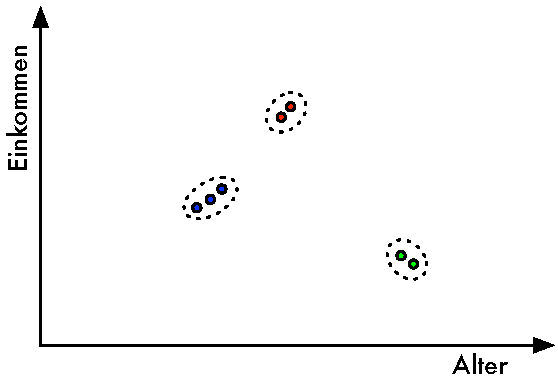
\includegraphics[scale=.7]{fig1/clustering.pdf}
\end{minipage}

\end{frame}

%---------------------------------------------------------------------

\begin{frame}
\frametitle{Sequenzanalyse}

\begin{itemize}
\item Suche nach häufig auftretenden Episoden oder Ereignisfolgen in
  Datenbeständen mit (zeitlicher) Ordnung
\begin{itemize}
\item Menge von Ereignistypen $E$, Sequenz von Paaren $(e, t$) mit $e
  \in E$ und $t$ ist Zeitstempel
\item Episode $\alpha$: partielle Ordnung von Ereignistypen
\item Häufigkeit einer Episode $\alpha$: Anzahl der Partition der
  Sequenz einer vorgegebenen Länge mit den durch $\alpha$ gegebenen
  Ereignistypen und deren Ordnung
\end{itemize}

\item Anwendungen
\begin{itemize}
\item Analyse von Alarmmeldungen (Events) in
  Telekommunikationssystemen
\item Web Usage Mining / Clickstream-Analyse
\item (zeitliches) Kaufverhalten, z.B.
 "`Herr der Ringe (DVD)"'
  $\longrightarrow$ "`Herr der Ringe (Buch)"' $\longrightarrow$
  "`Silmarillion"'
\end{itemize}
\end{itemize}

\end{frame}

%---------------------------------------------------------------------

\begin{frame}
\frametitle{Graph Mining: Analyse sozialer Netzwerke}

\begin{itemize}
\item Freundschaftsbeziehungen in sozialen Netzen wie Facebook,
  Follower in Twitter, \dots
\end{itemize}

\begin{minipage}[c]{4.5cm}
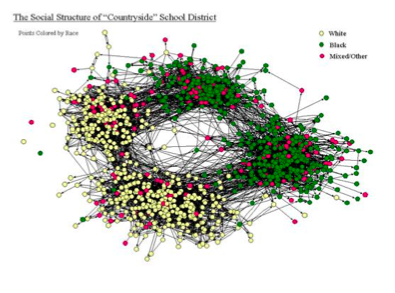
\includegraphics[width=4.5cm]{fig1/graph.png}
\end{minipage}\quad
\begin{minipage}[c]{5.5cm}
{\small
\begin{itemize}
\item Auffinden von Communities: Gruppen mit starken innerem
  Zusammenhang
\item Identifzieren von Autoritäten: wichtige Knoten/Peers (Personen)
  im Netzwerk
\item Link-Vorhersage und virales Marketing: Modellierung und
  Vorhersage von Diffusionsprozessen
\end{itemize}}
\end{minipage}

\end{frame}

%---------------------------------------------------------------------

\begin{frame}
\frametitle{Weitere Aufgabenstellungen}

\begin{itemize}
\item \hl{Text Mining:} Analyse von un- oder schwachstrukturierten Textdaten zur Aufdeckung von Semantik und Strukturen
\begin{itemize}
\item Dokumentenrepräsentation und Dokument-Clustering
\item Informationsextraktion: Entity Recognition, Sentiment-Analyse, \dots
\item Natural Language Processing
\end{itemize}
\item \hl{Spatio-Temporal Mining:} Analyse von Daten mit räumlichem
  und/oder zeitlichem Bezug
\begin{itemize}
\item Muster: räumliche Ausreißer (z.B. Stauzonen in Verkehrsnetzen),
  Vorhersage von Lokation/Bewegung (zur Optimierung von
  Transportsystemen), räumliche Cluster, Ko-Lokationen
\end{itemize}
\end{itemize}
\end{frame}


%---------------------------------------------------------------------

\begin{frame}
\frametitle{Zusammenfassung}

\begin{itemize}
\item \hl{Grundlagen des Data-Science-Prozesses}
\begin{itemize}
\item Motivation
\item mehrere Phasen und iteratives Vorgehen
\end{itemize}
\item \hl{Anwendungsfälle}
\begin{itemize}
\item Auswertung empirisch erfasster Daten
\item Analyse betriebswirtschaftlicher Daten, wissenschaftlicher
  Daten, Netzwerkdaten (Intrusion Detection, Web Mining, Web Log
  Mining), \dots
\item aber auch Textanalyse (Textklassifikation), Bildanalyse
  (Clustering von Bildern), \dots
\end{itemize}
\end{itemize}

\end{frame}

%---------------------------------------------------------------------

%%% Local Variables:
%%% mode: latex
%%% TeX-master: "main"
%%% End:

%%%%%%%%%%%%%%%%%%%%%%%%%%%%%%%%%%%%%%%%%%%%%%%%%%%%%%%%%%%%%%%%%%%%%%

\part{Werkzeuge zur Datananalyse: SQL, Python, Jupyter}

\frame[plain,c]{\partpage}

\frame{
  \frametitle{Überblick}
%  \tableofcontents[currentsection,hidesubsections,firstsection=12]
  \tableofcontents[firstsection=9]
}

\frame{
  \frametitle{Motivation}

  }

    %--------------------------------------------------------------

\frame{
  \frametitle{Motivation /2}

  \begin{itemize}
    \item Datenbanksysteme bieten umfassende Möglichkeiten zur Datenverarbeitung und -analyse
    \begin{itemize}
      \item effiziente Verwaltung (Indexstrukturen, Speicherverwaltung, Fehlersicherheit, Replikation, \dots)
      \item Konsistenzsicherung (Integritätsbedingungen, \dots)
      \item Datenmodellierung
      \item mächtige, deklarative Anfragesprache (SQL)
      \item optimierte Ausführung (Anfrageoptimierung, Parallelisierung, \dots)
    \end{itemize}
    \item \hl{In-Database Analytics} statt Datenexport und/oder dateibasierter Analyse?
  \end{itemize}

  }

  %--------------------------------------------------------------

\frame{
    \frametitle{Datenbank- oder dateibasierte Analyse?}
  
  \begin{columns}[t]
    \begin{column}{0.1\textwidth}
    \hl{Datenbank:}
    \end{column}
    \begin{column}{0.8\textwidth}
      \vspace*{-1.6em}
    \begin{itemize}
      \item Daten bereits in DBMS vorhanden
      \item Daten sind langfristig zu verwalten; werden regelmäßig aktualisiert
      \item wiederholte Analysen
      \item \hl{Import-Aufwand} lohnt sich
    \end{itemize}
  \end{column}
  \end{columns}
  \bigskip
  
  \begin{columns}[t]
    \begin{column}{0.1\textwidth}
    \hl{Dateibasiert:}
  \end{column}
  \begin{column}{0.8\textwidth}
    \vspace*{-1.6em}
      \begin{itemize}
      \item kleinere Datenmengen
      \item schwach strukturierte Daten
      \item nur einmalige Analyse
      \item Analyseverfahren erfordern Datenexport (z.B. Data Mining-Verfahren)
      \item \hl{Import-Aufwand} größer als Analyseaufwand
    \end{itemize}
  \end{column}
  \end{columns}
    }
  

\section{Datenimport mit SQL-DBMS}

\begin{frame}

\frametitle{Laden}

\begin{itemize}
\item Aufgabe
\begin{itemize}
\item Effizientes Einbringen von externen Daten in DBS
\end{itemize}
\item Kritischer Punkt
\begin{itemize}
\item Ladevorgänge blockieren unter Umständen Teile des DBS
\end{itemize}
\item Aspekte
\begin{itemize}
\item Trigger
\item Integritätsbedingungen
\item Indexaktualisierung
\item Update oder Insert?
\end{itemize}
\end{itemize}

\end{frame}

%--------------------------------------------------------------

\begin{frame}

\frametitle{Satzbasiert}

\begin{itemize}
\item Benutzung von Standard-Schnittstellen: \\JDBC, ODBC, \dots
\item Arbeitet im normalen Transaktionskontext
\item Trigger, Indexe und Constraints bleiben aktiv
\begin{itemize}
\item Manuelle Deaktivierung möglich
\end{itemize}
\item Keine großräumigen Sperren
\item Sperren können durch \op{COMMIT} verringert werden
\begin{itemize}
\item Nicht bei DBMS mit MVCC: Leseoperationen werden nie gesperrt 
\end{itemize}
\item Benutzung von Prepared Statements
\item Teilweise proprietäre Erweiterungen (Arrays) verfügbar
\end{itemize}

\end{frame}

%--------------------------------------------------------------

\begin{frame}

    \frametitle{DB-Import am Beispiel von PostgreSQL}
    
\end{frame}

%--------------------------------------------------------------

\begin{frame}

    \frametitle{Multi-Table-Insert in Oracle}
    
    \begin{itemize}
    \item Einfügen in mehrere Tabellen bzw. mehrfach (z.B. für Pivoting)
    
    \hspace*{-1cm}\begin{sql}
    \op{INSERT ALL} \\
    \op{INTO} Quartal\_Verkauf \\
    \1 \op{VALUES} (Produkt\_Nr, Jahr || '/Q1', Umsatz\_Q1) \\
    \op{INTO} Quartal\_Verkauf \\
    \1 \op{VALUES} (Produkt\_Nr, Jahr || '/Q2', Umsatz\_Q2) \\
    \op{INTO} Quartal\_Verkauf \\
    \1 \op{VALUES} (Produkt\_Nr, Jahr || '/Q3', Umsatz\_Q3) \\
    \op{INTO} Quartal\_Verkauf \\
    \1 \op{VALUES} (Produkt\_Nr, Jahr || '/Q4', Umsatz\_Q4) \\
    \op{SELECT} \dots\ \op{FROM} \dots
    \end{sql}
    \end{itemize}
    
    \end{frame}
    
    %--------------------------------------------------------------
    
    \begin{frame}
    
    \frametitle{Multi-Table-Insert in Oracle /2}
    
    \begin{itemize}
    \item Bedingtes Einfügen
    
    \hspace*{-1cm}\begin{sql}
    \op{INSERT ALL} \\
    \op{WHEN} ProdNr \op{IN} \\
    \1 (\op{SELECT} ProdNr \op{FROM} Werbe\_Aktionen) \\
    \op{INTO} Aktions\_Verkauf \\
    \1 \op{VALUES} (ProdNr, Quartal, Umsatz) \\
    \op{WHEN} Umsatz > 1000 \\
    \1 \op{INTO} Top\_Produkte \op{VALUES} (ProdNr) \\
    \op{SELECT} \dots\ \op{FROM} \dots
    \end{sql}
    
    \end{itemize}
    
    \end{frame}
    
    %--------------------------------------------------------------
    
    \begin{frame}
    
    \frametitle{Merge in SQL}
    
    \begin{itemize}
    \item Merge: Versuch eines Inserts, bei Fehler (durch Verletzung einer
      Schlüsselbedingung) $\rightarrow$ Update
    \hspace*{-1cm}\begin{sql}
    \op{MERGE INTO} Kunden K \op{USING} Neukunden N \\
    \op{ON} (N.Name = K.Name \op{AND} N.GebDatum = K.GebDatum) \\
    \op{WHEN MATCHED THEN} \\
    \op{UPDATE SET} K.Name = N.Name, K.Vorname=N.Vorname, \\
    \1 K.GebDatum=N.GebDatum \\
    \op{WHEN NOT MATCHED THEN} \\
    \op{INSERT VALUES} (MySeq.NextVal, N.Name, \\
    \1 N.Vorname, N.GebDatum)
    \end{sql}
    
    \end{itemize}
    
    \end{frame}

    %--------------------------------------------------------------
    
\section{Datenanalyse mit SQL}

\begin{frame}
    \frametitle{Gruppierung und Aggregation}
    
    \begin{itemize}
    \item Datenanalyse: Aggregation mehrdimensionaler Daten
    \item Aggregatfunktion: "`dimensionsfreie"' Antwort
    \begin{itemize}
    \item Standard: \op{SUM}, \op{MIN}, \op{MAX}, \op{COUNT}
    \item Erweiterungen: statistische, physikalische und Finanzfunktionen
    \item Benutzerdefinierte Aggregatfunktionen
    \end{itemize}
    \item Gruppierung: "`1-dimensionale"' Antwort
    \begin{itemize}
    \item Ergebnis: Tabelle mit Aggregatwerten indiziert durch Menge von Attributen
    \end{itemize}
    \end{itemize}
    
    \end{frame}
    
    %---------------------------------------------------------------------
    
    \begin{frame}
    \frametitle{Gruppierung und Aggregation (2)}
    
    \begin{itemize}
    \item SQL: \op{GROUP BY}\emph{ attrib\_liste} [ \op{HAVING} \emph{bedingung} ]
    \begin{itemize}
    \item Gruppierung bzgl. gleicher Werte der Gruppierungsattribute
    \item Abschließende Projektion nur über Gruppierungsattribute oder
      Aggregationen
    \end{itemize}
    \item Einschränkungen
    \begin{itemize}
    \item Berechnung von Histogrammen: Aggregationen über berechnete
      Kategorien\\
    \texttt{... \op{GROUP BY} func(Zeit) \op{AS} Woche ...}
    \item Berechnung von Zwischen- und Gesamtsummen
    \item Berechnung von Kreuztabellen
    \end{itemize}
    \end{itemize}
    
    \end{frame}
    
    %---------------------------------------------------------------------
    \begin{frame}
    \frametitle{Aggregatfunktionen}
    
    \begin{itemize}
    \item Standard-SQL-Funktionen wie \op{MIN}, \op{MAX}, \op{SUM},
      \op{COUNT}, \op{AVG}
    \item neue Funktionen in SQL:2003 für Varianz
      \texttt{\op{VAR\_POP}($x$)}, Standardabweichung \texttt{\op{STDDEV\_POP}($x$)},
      Kovarianz \texttt{\op{COVAR\_POP}($x$, $y$)}  und
      Korrelationskoeffizienten  \texttt{\op{CORR}($x$, $y$)}
    \item jeweils für die gesamte Population (\op{\_POP}) bzw. mit
      Bessel-Korrektur (\op{\_SAMP})
    \end{itemize}
    
    \end{frame}
    
    %---------------------------------------------------------------------
    
    \begin{frame}
    \frametitle{Aggregatfunktionen: Beispiele}
    
    \begin{itemize}
    \item Existiert ein (linearer) Zusammenhang zwischen Anzahl der
      verkauften Produkte und deren Verkaufspreis?
    \end{itemize}
    
    \begin{sql}
    \op{SELECT} \op{COVAR\_POP}(V\_Anzahl, P\_Verkaufspreis) \\
    \op{FROM} Verkauf, Produkt \\
    \op{WHERE} V\_Produkt\_ID = P\_ID
    \end{sql}
    
    \begin{itemize}
    \item Werte nahe Null $\approx$ nicht stärker als statistischer Zufall
    \end{itemize}
    
    \end{frame}
    
    %---------------------------------------------------------------------
    
    \begin{frame}
    \frametitle{Aggregatfunktionen: Beispiele}
    
    \begin{itemize}
    \item Kovarianz gibt keinen Aufschluss über Stärke der Korrelation,
      besser Korrelationskoeffizient
    \end{itemize}
    
    \begin{sql}
    \op{SELECT} \op{CORR}(P\_Verkaufspreis, P\_Einkaufspreis), \\
    \> P\_Produktgruppe \\
    \op{FROM} Verkauf, Produkt \\
    \op{WHERE} V\_Produkt\_ID = P\_ID \\
    \op{GROUP BY} P\_Produktgruppe
    \end{sql}
    
    \begin{itemize}
    \item Werte ab $0{,}5$ deuten auf mittlere bis starke Korrelation
    \end{itemize}
    
    \end{frame}
    
    %---------------------------------------------------------------------
    
    \begin{frame}[shrink]
    \frametitle{Aggregatfunktionen: Beispiele}
    
    \begin{itemize}
    \item Regressionsanalyse für Zusammenhang zwischen Anzahl und
      Verkaufspreis
    \item Berechnung von Geradenanstieg \op{REGR\_SLOPE},
      Regressionskoeffizienten \op{REGR\_R2}, mittleren Preis
      \op{REGR\_AVGX} und mittlere Anzahl \op{REGR\_AVGY}
    \end{itemize}
    
    {\begin{sql}
    \op{SELECT} V\_Kanal, \\
    \1\op{REGR\_SLOPE}(V\_Anzahl, P\_Verkaufspreis) \op{AS}
    Anstieg, \\
     \1\op{REGR\_R2}(V\_Anzahl, P\_Verkaufspreis) \op{AS} Koeff, \\
      \1\op{REGR\_COUNT}(V\_Anzahl, P\_Verkaufspreis) \op{AS} Anzahl, \\
      \1\op{REGR\_AVGX}(V\_Anzahl, P\_Verkaufspreis) \op{AS} MPreis, \\
      \1\op{REGR\_AVGY}(V\_Anzahl, P\_Verkaufspreis) \op{AS} MAnzahl \\
    \op{FROM} Verkauf, Produkt, Zeit \\
    \op{WHERE} V\_Produkt\_ID = P\_ID \op{AND} \\
    V\_Zeit\_ID = Z\_ID \op{AND} \op{YEAR}(Z\_Datum) = 2011 \\
    \op{GROUP BY} V\_Kanal
    \end{sql}}
    
    \end{frame}
    
    %---------------------------------------------------------------------
    
    \begin{frame}
    \frametitle{Berechnung von Zwischen- und Gesamtsummen}
    
    
    {\begin{center}\begin{scriptsize}
    \begin{tabular}{|c|c|l|c|c|c|c|}
    \hline
    \rowcolor{Gray} {PGruppe} & {Jahr} & {Bundesland} & {Umsatz} & {Umsatz} & {Umsatz} & {Umsatz} \\
    \rowcolor{Gray}      &      &        & {PGruppe-} & {PGruppe-} &  {PGruppe} & \\
    \rowcolor{Gray}      &      &        & {Jahr-}  & {Jahr}  &  & \\
    \rowcolor{Gray}      &      &        & {Bundesland} &       &  & \\
    \hline\hline
    {Wein} & {2010} & {Sachsen-Anhalt} & {45}    &       &  & \\
            &      & {Th"uringen} & {43}    &       &  & \\
    \hline
            &      &      &        & {88}   &  & \\
    \hline
            & {2011} & {Sachsen-Anhalt} & {47}    &       &  & \\
    \hline
            &      &      &        & {47}   &  & \\
    \hline
            &      &      &        &       & {135}  & \\
    \hline
    {Bier} & {2011} & {Th{\"u}ringen} & {42}    &       &  & \\
    \hline
            &      &      &        & {42}   &  & \\
    \hline
            &      &      &        &       & {42}  & \\
    \hline
            &      &      &        &       &   & {177}\\
    \hline
    \end{tabular}\end{scriptsize}
    \end{center}}
    %
    %{\scriptsize\begin{center}
    %\begin{tabular}{|c|c|c|c|c|c|}
    %\hline
    %Produkt & Jahr & Region & Verk. & Verk. & Verk. \\
    %      &      &        & Prod.- & Prod. & Prod. \\
    %      &      &        & Jahr-  & Jahr  & \\
    %      &      &        & Region &       & \\
    %\hline\hline
    %Rotwein & 2010 & SANH & 135    &       & \\
    %        &      & THÜR & 120    &       & \\
    %        &      &      &        & 255   & \\
    %        & 2011 & SANH & 140    &       & \\
    %        &      & THÜR & 135    &       & \\
    %        &      &      &        & 275   & \\
    %        &      &      &        &       & 530 \\
    %\hline
    %\end{tabular}
    %\end{center}}
    %% Tabelle
    %
    %{\scriptsize\begin{center}
    %\begin{tabular}{|c|c|c|c|}
    %\hline
    %Produkt & Jahr & Region & Verkäufe \\
    %\hline \hline
    %Rotwein & 2010 & SANH & 135 \\
    %Rotwein & 2010 & THÜR & 120 \\
    %Rotwein & 2010 & \ALLresult & 255 \\
    %Rotwein & 2011 & SANH & 140 \\
    %Rotwein & 2011 & THÜR & 135 \\
    %Rotwein & 2011 & \ALLresult & 275 \\
    %Rotwein & \ALLresult & \ALLresult & 530 \\
    %\hline
    %\end{tabular}
    %\end{center}}
    
    \end{frame}
    
    %---------------------------------------------------------------------
    
    \begin{frame}[shrink=10]
    \frametitle{Berechnung von Zwischen- und Gesamtsummen (2)}
    %
    %\begin{sql}
    %  \op{SELECT} Produkt, \op{NULL}, \op{NULL}, \op{SUM}(Verkäufe)\\
    %  \1	\op{FROM} Verkauf\\
    %  \1	\op{WHERE} Produkt = 'Beaujolais'\\
    %  \1	\op{GROUP BY} Produkt\\
    %  \op{UNION}\\
    %  \op{SELECT} Produkt, Jahr, \op{NULL}, \op{SUM}(Verkäufe)\\
    %  \1	\op{FROM} Verkauf\\
    %  \1	\op{WHERE} Produkt = 'Beaujolais'\\
    %  \1	\op{GROUP BY} Produkt, Jahr\\
    %  \op{UNION}\\
    %  \op{SELECT} Produkt, Jahr, Region, \op{SUM}(Verkäufe)\\
    %  \1	\op{FROM} Verkauf\\
    %  \1	\op{WHERE} Produkt = 'Beaujolais'\\
    %  \1 \op{GROUP BY} Produkt, Jahr, Region
    %\end{sql}
    
    \begin{sql}
    -{}- \ccomment{Zwischensumme (1) "uber alle Produktgr., Jahre und Bundesl"ander} \\
    \op{SELECT} P\_Produktgruppe  \op{AS} PGruppe, \op{YEAR}(Z\_Datum), \\
    \1 O\_Bundesland, \op{SUM}(V\_Anzahl * P\_Verkaufspreis) \op{AS} Umsatz \\
    \op{FROM}  Verkauf, Zeit, Produkt, Ort \\
    \op{WHERE}  V\_Zeit\_ID = Z\_ID \op{AND} V\_Produkt\_ID = P\_ID \op{AND} \\
    \1 V\_Ort\_ID = O\_ID \\
    \op{GROUP BY} P\_Produktgruppe, \op{YEAR} (Z\_Datum), O\_Bundesland \\
      \op{UNION ALL} \\
    -{}- \ccomment{Zwischensumme (2) "uber alle Produktgruppen und  Jahre} \\
    \op{SELECT}  P\_Produktgruppe \op{AS} PGruppe, \op{YEAR} (Z\_Datum), \\
    \1 \op{CAST}(\op{NULL AS VARCHAR(50)}), \\
    \1 \op{SUM}(V\_Anzahl * P\_Verkaufspreis) \op{AS} Umsatz  \\
    \op{FROM}  Verkauf, Zeit, Produkt, Ort \\
    \op{WHERE}  V\_Zeit\_ID = Z\_ID \op{AND} V\_Produkt\_ID = P\_ID \op{AND} \\
    \1 V\_Ort\_ID = O\_ID \\
     \op{GROUP BY} P\_Produktgruppe, \op{YEAR}(Z\_Datum)  \\
      \op{UNION ALL}  \\
    \end{sql}
    
    \end{frame}
    
    
    
    %---------------------------------------------------------------------
    
    \begin{frame}[shrink=10]
    \frametitle{Berechnung von Zwischen- und Gesamtsummen (3)}
    
    \begin{sql}
    -{}- \ccomment{Zwischensumme (3) "uber alle Produktgruppen} \\
    \op{SELECT}  P\_Produktgruppe  \op{AS} PGruppe, \op{CAST}(\op{NULL AS  INT}), \\
    \1 \op{CAST}(\op{NULL AS VARCHAR(50)}), \\
    \1 \op{SUM}(V\_Anzahl * P\_Verkaufspreis) \op{AS} Umsatz  \\
    \op{FROM}  Verkauf, Zeit, Produkt, Ort \\
    \op{WHERE} V\_Zeit\_ID = Z\_ID \op{AND} V\_Produkt\_ID = P\_ID \op{AND} \\
    \1 V\_Ort\_ID = O\_ID \\
    \op{GROUP BY} P\_Produktgruppe  \\
     \op{UNION ALL}  \\
    -{}- \ccomment{Gesamtsumme} \\
    \op{SELECT}  \op{CAST}(\op{NULL AS VARCHAR(50)})  \op{AS} PGruppe, \\
    \1 \op{CAST}(\op{NULL AS INT}), \\
    \1 \op{CAST}(\op{NULL AS VARCHAR(50)}), \\
    \1 \op{SUM}(V\_Anzahl * P\_Verkaufspreis) \op{AS} Umsatz  \\
    \op{FROM}  Verkauf, Zeit, Produkt, Ort \\
    \op{WHERE}  V\_Zeit\_ID = Z\_ID \op{AND} V\_Produkt\_ID = P\_ID \op{AND} \\
    \1 V\_Ort\_ID = O\_ID
     \end{sql}
    
    \end{frame}
    
    %---------------------------------------------------------------------
    
    
    \begin{frame}
    \frametitle{Ausschnitt der Zwischen- und Gesamtsummen}
    
    {\begin{center}
    \begin{tabular}{|l|c|l|r|l}
    \hline
    \rowcolor{Gray} {PGruppe} & {Jahr} &  {O\_Bundesland} &  {Umsatz} \\
    \hline \hline
     {Wein} &  {2010} &  {Sachsen-Anhalt} &  {45} \\
     {Wein} &  {2010} &  {Th"uringen} &  {43} \\
     {Wein} &  {2011} &  {Sachsen-Anhalt} &  {47} \\
     {Bier} &  {2011} &  {Th"uringen} &  {42} \\
    \hline
     {Wein} &  {2010} & $NULL$ &  {88} \\
     {Wein} &  {2011} & $NULL$ &  {47} \\
     {Bier} &  {2011} & $NULL$ &  {42} \\
    \hline
     {Wein} & $NULL$ & $NULL$ &  {135} \\
     {Bier} & $NULL$ & $NULL$ &  {42} \\
    \hline
    $NULL$ & $NULL$ & $NULL$ &  {177} \\
    \hline
    \end{tabular}
    \end{center}}
    
    \end{frame}
    
    %---------------------------------------------------------------------
    
    \begin{frame}
    \frametitle{Nachteile der UNION-Variante}
    
    \begin{itemize}
    \item Hoher Aufwand:
    \begin{itemize}
    \item Berechnung aller Teilsummen für $n$ Gruppierungsattribute
      erfordert $2^n$ Teilanfragen
    \item Eventuelle Verbundoperationen müssen mehrfach wiederholt werden
    \end{itemize}
    \item Aufwendige Formulierung:
    \begin{itemize}
    \item Jedoch eventuell Generierung durch OLAP-Werkzeuge
    \item Einhalten der Struktur
    \end{itemize}
    \end{itemize}
    \end{frame}
    
    %---------------------------------------------------------------------
    
    \begin{frame}
    \frametitle{Berechnung von Kreuztabellen}
    
    \begin{itemize}
    \item Symmetrische Aggregation
    \item Auch Pivot-Tabellen
    \end{itemize}
    
    \begin{center}
    \begin{tabular}{|l||c|c|c|}
    \hline
    \rowcolor{Gray} Verkäufe & 2010 & 2011 & Gesamt \\
    \hline \hline
    Thüringen & 120 & 135 & 255 \\
    \hline
    Sachen-Anhalt & 135 & 140 & 275 \\
    \hline
    Gesamt & 255 & 275 & 530 \\
    \hline
    \end{tabular}
    \end{center}
    
    \end{frame}
    
    %---------------------------------------------------------------------
    
    \begin{frame}
    \frametitle{PIVOT in SQL Server}
    
    \begin{sql}
      \op{SELECT} Jahr, [THÜR] \op{AS} Thüringen, \\
      \1 [SANH] \op{AS} Sachsen-Anhalt \\
      \op{FROM} Verkauf \\
      \op{PIVOT} (\op{SUM}(Verkäufe) \op{FOR} \\
      \1 Region \op{IN} ([THÜR], [SANH]))
    \end{sql}
    
    \begin{center}
    \begin{tabular}{|c|c|c|}
    \hline
    \rowcolor{Gray} Jahr & Thüringen & Sachsen-Anhalt \\
    \hline
    \hline
    2010 & 135 & 120 \\
    \hline
    2011 & 140 & 135 \\
    \hline
    \end{tabular}
    \end{center}
    
    \end{frame}
    
    %---------------------------------------------------------------------
    \begin{frame}
    \frametitle{Cube-Operator}
    \begin{itemize}
    \item "`Kurzform"' für Anfragemuster zur Berechnung von Teil- und
      Gesamtsummen
    \item Generierung aller möglichen Gruppierungskombinationen aus
      gegebener Menge von Gruppierungsattributen
    \item Ergebnis: Tabelle mit aggregierten Werten
    \item Gesamtaggregat:
      $$
      \texttt{NULL}, \texttt{NULL}, ..., \texttt{NULL}, f(*)
      $$
    \item Höherdimensionale Ebenen mit weniger \texttt{NULL}-Werten
    \end{itemize}
    
    \end{frame}
    
    %%%%%%%%%%%%%%%%%%%%%%%%%%%%%%%%%%%%%%%%%%%%%%%%%
    
    \begin{frame}[shrink=10]
    
    \frametitle{Cube-Operator: Beispiel}
    
    \begin{minipage}{5.4cm}
    {\tiny
    \begin{tabular}{|l|c|c|c|}
    \hline
    \rowcolor{Gray} \textbf{PGruppe} & \textbf{Bundesland} & \textbf{Jahr} & \textbf{Umsatz} \\
    \hline\hline
    Wein & Sachsen-Anhalt & 2010 & 45 \\
    \hline
    Wein & Thüringen & 2010 & 43 \\
    \hline
    Wein & Sachsen-Anhalt & 2011 & 47 \\
    \hline
    Bier & Thüringen & 2011 & 42 \\
    \hline
    \end{tabular}}
    \end{minipage}%
    \begin{minipage}{1.4cm}
    
\includegraphics[scale=.46]{fig3/Cube-Pfeil.pdf}
    \end{minipage}%
    \begin{minipage}{4cm}
    {\tiny
    \begin{tabular}{|l|l|l|r|}
    \hline
    \rowcolor{Gray} \textbf{PGruppe} & \textbf{Jahr} & \textbf{Bundesland} & \textbf{Umsatz} \\
    \hline\hline
     {Wein} &  {2010} &  {Sachsen-Anhalt} &  {45} \\
    \hline
     {Wein} &  {2010} &  {Th"uringen} &  {43} \\
    \hline
    \dots & \dots & \dots & \dots \\
    \hline
     {Wein} &  {2010} & {NULL} & {88} \\
    \hline
    {Wein} & {2011} & {NULL} & {47} \\
    \hline
    {Bier} & {2011} & {NULL} & {42} \\
    \hline
    {Wein} & {NULL} & {Sachsen-Anhalt} & {92} \\
    \hline
    {Wein} & {NULL} & {Th"uringen} & {43} \\
    \hline
    {Bier} & {NULL} & {Th"uringen} & {42} \\
    \hline
    {Wein} & {NULL} & {NULL} & {135} \\
    \hline
    {Bier} & {NULL} & {NULL} & {42} \\
    \hline
    {NULL} & {2010} & {Sachsen-Anhalt} & {45} \\
    \hline
    \dots & \dots & \dots & \dots \\
    \hline
    {NULL}& {NULL} & {Sachsen-Anhalt} & {92} \\
    \hline
    {NULL} & {NULL} & {Thüringen} & {85} \\
    \hline
    \dots & \dots & \dots & \dots \\
    \hline
    {NULL} & {2010} & {NULL} & {88} \\
    \hline
    {NULL} & {2011} & {NULL} & {89} \\
    \hline
    {NULL} & {NULL} & {NULL} & {177} \\
    \hline
    \end{tabular}}
    \end{minipage}%
    
    
    \end{frame}
    
    %%%%%%%%%%%%%%%%%%%%%%%%%%%%%%%%%%%%%%%%%%%%%%
    
    \begin{frame}
    
    \frametitle{Cube: Details}
    \begin{itemize}
    \item Kardinalität
      \begin{itemize}
      \item $N$ Attribute mit Kardinalität $C_1, C_2, ..., C_N$
      \item Gesamtkardinalität des \op{CUBE}:
      $$
       \prod_{i=1}^{N}(C_i+1)
      $$
      \end{itemize}
    \item Anzahl der Super-Aggregatwerte
      \begin{itemize}
      \item $N$ Attribute in der \op{SELECT}-Klausel
      \item Super-Aggregate: $2^N-1$
      \end{itemize}
    \end{itemize}
    \end{frame}
    
    %%%%%%%%%%%%%%%%%%%%%%%%%%%%%%%%%%%%%%%%%%%%%%
    
    \begin{frame}
    
    \frametitle{Cube-Operator: SQL-Syntax}
    \begin{itemize}
    \item Implementierung in SQL Server, DB2, Oracle
    \end{itemize}
    
    \begin{sql}
        \textbf{SELECT} P\_Produktgruppe \op{AS} PGruppe,\\
     \1 O\_Bundesland, YEAR(Z\_Datum),\\
     \1 \textbf{SUM}(V\_Anzahl * P\_Verkaufspreis) \op{AS} Umsatz\\
        \textbf{FROM} Verkauf, Zeit, Produkt, Ort\\
        \textbf{WHERE} \dots \\
        \textbf{GROUP BY CUBE}(P\_Produktgruppe, O\_Bundesland, \\
    \1 \op{YEAR}(Z\_Datum))
      \end{sql}
    
    \end{frame}
    
      \begin{frame}
    
        \frametitle{Cube-Operator: SQL-Syntax /2}
        \begin{itemize}
    \item Funktion \op{GROUPING}(Attribut)
      \begin{itemize}
      \item Liefert Wert = 1, wenn über Attribut aggregiert wurde
      \item Liefert Wert = 0, wenn nach Attribut gruppiert wurde
      \end{itemize}
    \item Unterdrückung von Teilsummen, z.B. der Gesamtsumme
    \end{itemize}
    
    \begin{sql}
        ... \textbf{HAVING NOT} (\=
        \textbf{GROUPING}(P\_Produktgruppe) = 1 \textbf{AND}\\
        \1  \textbf{GROUPING}(O\_Bundesland) = 1 \textbf{AND}\\
        \1 \textbf{GROUPING}(YEAR(Z\_Datum)) = 1)
    \end{sql}
    
    \end{frame}
    
    %%%%%%%%%%%%%%%%%%%%%%%%%%%%%%%%%%%%%%%%%%%%%%
    \begin{frame}
    
    \frametitle{Rollup-Operator}
    
    
    \begin{itemize}
    \item \op{CUBE}-Operator: \hl{interdimensional}
      \begin{itemize}
      \item anwendbar für Attribute aus unterschiedlichen Dimensionen
      \item Für Roll-Up oder Drill-Down-Operationen zu aufwendig
      \end{itemize}
    \item \op{ROLLUP}-Operator: \hl{intradimensional}
      \begin{itemize}
      \item Generierung der Attributkombinationen
    $$
    (A_1, ..., A_N), (A_1, ..., A_{N-1}), (A_1, A_2), (A_1), ()
    $$
    für gegebene Attribut\textit{liste} $A_1, ..., A_N$
    \end{itemize}
    \end{itemize}
    
    \end{frame}
    
    
    %%%%%%%%%%%%%%%%%%%%%%%%%%%%%%%%%%%%%%%%%%%%%
    
    \begin{frame}
    
    \frametitle{ROLLUP-Operator: Beispiel (einfach)}
    
    
    \begin{itemize}
    \item Anfrage:
    \end{itemize}
    
    \begin{sql}
    \op{SELECT}  P\_Gruppe, Z\_Tag, Z\_Monat, Z\_Jahr, \\
    \1 \op{SUM}(V\_Anzahl * P\_Verkaufspreis) \op{AS} Umsatz \\
    \op{FROM}  Verkauf, Zeit, Produkt, Ort \\
    \op{WHERE}   V\_Produkt\_ID = P\_ID \op{AND} V\_Ort\_ID = O\_ID \op{AND} \\
    \1   V\_Zeit\_ID = Z\_ID \op{AND} \op{YEAR}(Z\_Datum) = 2011 \op{AND}\\
    \1 P\_Produktgruppe = 'Rotwein' \\
    \op{GROUP BY ROLLUP}(Z\_Jahr, Z\_Monat, Z\_Tag)
    \end{sql}
    
    \vspace*{-1em}
    \begin{itemize}
    \item Auswertung:
      \begin{itemize}
      \item Rollup: \texttt{(Z\_Jahr,Z\_Monat,Z\_Tag),
          (Z\_Jahr,Z\_Monat),(Z\_Jahr),()}
      \end{itemize}
    \end{itemize}
    
    \end{frame}
    
    %%%%%%%%%%%%%%%%%%%%%%%%%%%%%%%%%%%%%%%%%%%%
    
    
    \begin{frame}[shrink=10]
    
    \frametitle{ROLLUP-Operator: Beispiel (einfach)}
    
    \begin{center}
      \begin{tabular}{|l|c|l|l|r|}
        \hline
        \rowcolor{Gray}     {Gruppe} & {Tag} & {Monat} & {Jahr} &
        {Umsatz} \\
        \hline
        \hline
         {Rotwein} &  {1} &  {Januar} &  {2011} & 100 \\
         {Rotwein} &  {2} &  {Januar} &  {2011} & 100 \\
        \dots & \dots & \dots & \dots & \dots \\
         {Rotwein} &  {31} &  {Januar} &  {2011} & 100 \\
         {Rotwein} &  {NULL} &  {Januar} &  {2011} & 2000 \\
         {Rotwein} &  {1} &  {Februar} &  {2011} & 100 \\
         {Rotwein} &  {2} &  {Februar} &  {2011} & 100 \\
        \dots & \dots & \dots & \dots & \dots \\
         {Rotwein} &  {28} &  {Februar} &  {2011} & 100 \\
         {Rotwein} &  {NULL} &  {Februar} &  {2011} & 2000 \\
        \dots & \dots & \dots & \dots & \dots \\
         {Rotwein} &  {NULL} &  {NULL} &  {2011} & 24000 \\
    %    \dots & \dots & \dots & \dots & \dots \\
         {Rotwein} &  {NULL} &  {NULL} &  {NULL} & 24000 \\
        \hline
      \end{tabular}
    \end{center}
    
    
    \end{frame}
    
    %%%%%%%%%%%%%%%%%%%%%%%%%%%%%%%%%%%%%%%%%%%%
    
    \begin{frame}
    
    \frametitle{ROLLUP-Operator: Beispiel (zusammengesetzt)}
    
    
    \begin{itemize}
    \item Anfrage:
    \end{itemize}
    \begin{sql}
    \op{SELECT}  P\_Kategorie, P\_Gruppe, O\_Land, O\_Region\\
    \1 \op{SUM}(V\_Anzahl) \op{AS} Verkäufe \\
    \op{FROM}  Verkauf, Zeit, Produkt, Ort \\
    \op{WHERE}  V\_Zeit\_ID = Z\_ID \op{AND} V\_Produkt\_ID = P\_ID \\
    \1 \op{AND}  V\_Ort\_ID = O\_ID \op{AND} \op{YEAR}(Z\_Datum) = 2011 \\
    \op{GROUP BY ROLLUP}(P\_Kategorie, P\_Gruppe), \\
    \1 \op{ROLLUP}(O\_Land, (O\_Region))
    \end{sql}
    
    \vspace*{-1em}
    \begin{itemize}
    \item Auswertung:
      \begin{itemize}
      \item 1. Rollup: \texttt{(P\_Kategorie,P\_Gruppe),
          (P\_Kategorie),()}
      \item 2. Rollup: \texttt{(O\_Land,O\_Region),(O\_Land),()}
      \item Kreuzprodukt beider Kombination
      \end{itemize}
    \end{itemize}
    
    \end{frame}
    
    %%%%%%%%%%%%%%%%%%%%%%%%%%%%%%%%%%%%%%%%%%%%
    
    
    
    \begin{frame}[shrink=10]
    
    \frametitle{ROLLUP-Operator: Beispiel (zusammengesetzt)}
    
    \begin{center}
      \begin{tabular}{|l|l|l|l|l|}
        \hline
        \rowcolor{Gray}     P\_Kategorie&	P\_Gruppe&	Land	&Region&	Verkäufe\\
        \hline
        \hline
        Wein	&Weißwein&	D&	SANH&	102\\
        Wein	&Rotwein&	D&	SANH&	98\\
        Wein &	NULL&	D&	SANH&	200\\
        ...	&...&	...&	...&	...\\
        Wein	&Weißwein&	D&	NULL&	541\\
        Wein	&Rotwein&	D	&NULL&	326\\
        Wein&	NULL	&D	&NULL&	867\\
        ...	&...&	...&	...&	...\\
        Wein &NULL& D & NULL& 1232\\
        ...	&...&	...&	...&	...\\
        NULL& NULL& D& NULL& 1432\\
        ...	&...&	...&	...&	...\\
        NULL &NULL& NULL& NULL& 3456\\
        \hline
      \end{tabular}
    \end{center}
    
    
    \end{frame}
    
    %%%%%%%%%%%%%%%%%%%%%%%%%%%%%%%%%%%%%%%%%%%%
    \begin{frame}
    
    \frametitle{CUBE- vs. ROLLUP-Operator}
    
    
    \begin{itemize}
    \item CUBE-Operator:
      \begin{itemize}
      \item Generiert alle $2^n$ Kombinationen:
        \begin{itemize}
        \item z.B. für 4 Gruppierungsattribute 16 Kombinationen
        \end{itemize}
      \end{itemize}
    \item ROLLUP-Operator:
      \begin{itemize}
      \item Generiert nur Kombinationen mit Superaggregaten:
        \begin{itemize}
        \item $(f_1, f_2, ..., f_n),$
        \item $ ...$
        \item $(f_1, NULL, ..., NULL),$
        \item $(NULL, NULL, ..., NULL)$
        \end{itemize}
      \item $n+1$ Kombinationen
      \end{itemize}
    \end{itemize}
    
    \end{frame}
    
    %%%%%%%%%%%%%%%%%%%%%%%%%%%%%%%%%%%%%%%%%%%%
    
    \begin{frame}
    
    \frametitle{GROUPING SETS}
    
    \begin{sql}
        \textbf{GROUP BY} ... \textbf{GROUPING SETS}
        (\textit{gruppierung})
      \end{sql}
    
      \begin{itemize}
    \item Gruppierung:
      \begin{itemize}
      \item Einfache Gruppierungskombination, z.B.: \texttt{(O\_Bundesland,
         O\_Stadt)}
      \item Komplexe Gruppierungsbedingung mit \textbf{\texttt{CUBE}} oder
        \op{ROLLUP}
      \end{itemize}
    \end{itemize}
    
    
    \end{frame}
    
    %%%%%%%%%%%%%%%%%%%%%%%%%%%%%%%%%%%%%%%%%%%%
    
    \begin{frame}
    
    \frametitle{GROUPING SETS: Beispiel}
    
    
    \begin{sql}
        ...\\
        \textbf{GROUP BY}\\
        \1	  \textbf{ROLLUP}(P\_Produktgruppe, P\_Produktkategorie),\hl{(1)}\\
        \1    \textbf{GROUPING SETS}((O\_Stadt), (O\_Bundesland)),\hl{(2)}\\
        \1    \textbf{GROUPING SETS}(		\\
        \2 \textbf{ROLLUP}(Jahr, Quartal, Monat), (Woche))\hl{(3)}
      \end{sql}
    
    \begin{itemize}
    \item Bedeutung
      \begin{itemize}
      \item[\hl{(1)}] entlang der Klassifikationshierarchie
      \item[\hl{(2)}] nur für Städte und Bundesländer
      \item[\hl{(3)}] Nutzung der Parallelhierarchie
        \texttt{(Jahr$\to$Quartal$\to$Monat)} sowie \texttt{(Woche)}
      \end{itemize}
    
    \end{itemize}
    
    
    \end{frame}
    
    
    \begin{frame}
    
      \frametitle{Effekt von \op{GROUPING SETS}: Beispieldaten}
    
      \begin{center}
      \begin{tabular}{|l|l|l|r|}
        \hline
      \rowcolor{Gray} \textbf{PGruppe} &  \textbf{Bundesland} & \textbf{Jahr} & \textbf{Umsatz} \\
    \hline\hline
    Bier &	Sachsen-Anhalt &	2010	& 51 \\
    Bier &	Sachsen-Anhalt &	2011 &	46 \\
    Bier &	Thüringen	& 2010	& 49 \\
    Bier &	Thüringen	& 2011	& 47 \\
    Wein &	Sachsen-Anhalt	& 2010	& 45 \\
    Wein &	Sachsen-Anhalt	& 2011 & 	47 \\
    Wein &	Thüringen	& 2010	& 43 \\
    Wein &	Thüringen	& 2011	& 42 \\
    \hline
      \end{tabular}
    \end{center}
    
    \end{frame}
    
    \begin{frame}
    
      \frametitle{Effekt von \op{GROUPING SETS}}
    
      Simulation von \op{ROLLUP}
      \begin{sql}
        \op{SELECT} Bundesland, Jahr, \op{SUM}(Umsatz) \op{FROM} Verkauf \\
        \op{GROUP BY GROUPING SETS}( \\
        \1 (PGruppe, Bundesland, Jahr), \\
        \1 (PGruppe, Bundesland), (PGruppe), ());
      \end{sql}
    
      {\small
      \begin{center}
        \begin{tabular}{|l|l|l|r|}
          \hline
        \rowcolor{Gray} \textbf{PGruppe} &  \textbf{Bundesland} & \textbf{Jahr} & \textbf{Umsatz} \\
      \hline\hline
      NULL & NULL & NULL & 323 \\
      Wein	& Thüringen	& 2010 &	43 \\
      Bier &	Thüringen	& 2010 &	49 \\
      Wein &	Thüringen & 	NULL &	43 \\
      Bier &	Thüringen	& NULL	 & 91 \\
      Wein		& NULL & NULL &			135 \\
      \multicolumn{4}{|c|}{\dots} \\
      \hline
        \end{tabular}
      \end{center}}
    
    \end{frame}
    
    \begin{frame}
    
      \frametitle{Effekt von \op{GROUPING SETS} /2}
    
    \begin{sql}
      \op{SELECT} Bundesland, Jahr, \op{SUM}(Umsatz) \op{FROM} Verkauf \\
      \op{GROUP BY CUBE}(Bundesland, Jahr)
    \end{sql}
    liefert 9 Tupel: (Thüringen, 2010), (Thüringen, 2011), (Sachsen-Anhalt, 2010), \dots (Thüringen, NULL), (Sachsen-Anhalt, NULL), (NULL, NULL)
    
    \begin{sql}
      \op{SELECT} PGruppe, \op{SUM}(Umsatz) \op{FROM} Verkauf \\
      \op{GROUP BY} PGruppe
    \end{sql}
    
    liefert 2 Tupel: Bier, Wein
    \end{frame}
    
    
    
    
    
    \begin{frame}
    
      \frametitle{Effekt von \op{GROUPING SETS} /3}
    
      mehrfache Gruppierung ohne \op{GROUPING SETS}
    
      \begin{sql}
        \op{SELECT} PGruppe, Bundesland, Jahr, \op{SUM}(Umsatz) \\
        \op{FROM} Verkauf \\
        \op{GROUP BY} PGruppe, \op{CUBE}(Bundesland, Jahr)
      \end{sql}
    
      berechnet \hl{Kreuzprodukt} der Gruppierungskombinationen $\leadsto$ $2 \cdot 9 = 18$ Kombinationen
    
    \end{frame}
    
    
    \begin{frame}
    
      \frametitle{Effekt von \op{GROUPING SETS} /4}
    
    mit \op{GROUPING SETS}
    
    \begin{sql}
      \op{SELECT} PGruppe, Bundesland, Jahr, \op{SUM}(Umsatz) \\
      \op{FROM} Verkauf \\
      \op{GROUP BY GROUPING SETS}(PGruppe, \\
      \1 \op{CUBE}(Bundesland, Jahr))
    \end{sql}
    
     berechnet \hl{Vereinigung} der Gruppierungskombinationen $\leadsto$ $2 + 9 = 11$ Kombinationen
    \end{frame}
    
    \begin{frame}
    
    \frametitle{SQL:2003 -- Sequenzbasierte Operationen}
    
    \begin{itemize}
    \item Seit SQL:1999 -- Erweiterung um OLAP-Funktionen zur attribut- und
      sequenzbasierten Auswertung
    \item Attribut- und tupelbasierte Aggregation
    \item Umsetzung u.a. in Oracle und DB2
    \item Unterstützte Anfragetypen
      \begin{itemize}
      \item Ratio-To-Total
      \item Laufende Summen (Kumulation)
      \item Gleitender Durchschnitt
      \item Ranking-Analyse
      \end{itemize}
    \end{itemize}
    
    \end{frame}
    
    %%%%%%%%%%%%%%%%%%%%%%%%%%%%%%%%%%%%%%%%%%%%
    
    
    \begin{frame}
    
    \frametitle{OLAP-Funktionen: Syntax}
    
    
    
    \begin{center}
      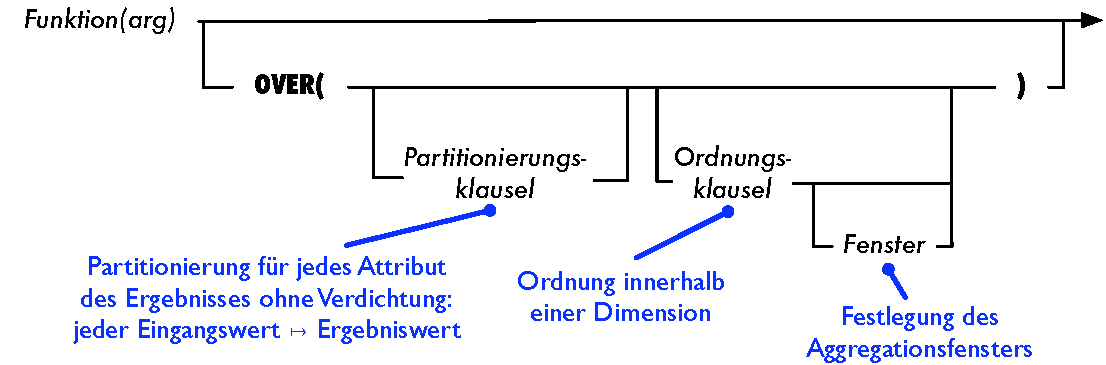
\includegraphics[scale=.6]{fig3/OLAP-Syntax.pdf}
    \end{center}
    
    
    \end{frame}
    
    
    %%%%%%%%%%%%%%%%%%%%%%%%%%%%%%%%%%%%%%%%%%%%
    
    \begin{frame}
    \frametitle{Sichtdefinition für folgende Beispiele}
    
    \begin{sql}
    \op{CREATE VIEW} TagesUmsatz \op{AS} \\
    \1 \op{SELECT} P\_Produktgruppe, Z\_Datum, \\
    \2 \op{SUM}(V\_Anzahl * P\_Verkaufspreis) \op{AS} Umsatz \\
    \1 \op{FROM} Verkauf, Zeit, Produkt \\
    \1 \op{WHERE} V\_Zeit\_Id = Z\_Id \op{AND} V\_Produkt\_Id = P\_Id \\
    \1 \op{GROUP BY} P\_Produktgruppe, Z\_Datum
    \end{sql}
    
    \end{frame}
    
    %%%%%%%%%%%%%%%%%%%%%%%%%%%%%%%%%%%%%%%%%%%%
    
    \begin{frame}
    \frametitle{OLAP-Funktionen: Motivation}
    
    \begin{itemize}
    \item \hl{Ratio-To-Total-Analyse}: Berechnung des Tagesumsatzes am Gesamtumsatz des Monats
      \item Klassische SQL-Anfrage:
    \end{itemize}
    
    \begin{sql}
    \op{SELECT} Z\_Datum, Umsatz,GesamtUmsatz \op{AS} MonatGesamt \\
    \1 100.0*Umsatz/GesamtUmsatz \op{AS} Anteil, \\
    \op{FROM}  TagesUmsatz, \\
    \1 (\op{SELECT} \op{SUM}(Umsatz) \op{AS} GesamtUmsatz \\
    \1 \op{FROM} TagesUmsatz \\
    \1 \op{WHERE} P\_Produktgruppe = 'Wein' \op{AND} \\
    \2 \op{YEAR\_MONTH}(Z\_Datum) = 201108)  Gesamt \\
    \op{WHERE}  P\_Produktgruppe = 'Wein' \op{AND} \\
    \1 \op{YEAR\_MONTH}(Z\_Datum) = 201108
      \end{sql}
    
    \end{frame}
    
    \begin{frame}
      \frametitle{OLAP-Funktionen: Motivation /2}
    
      \begin{itemize}
      \item Innere Unteranfrage berechnet die Gesamtmenge für die
        Anteilsberechnung:
      \end{itemize}
    
      \begin{sql}
          ( \= \op{SELECT} \op{SUM}(Umsatz) \op{AS} GesamtUmsatz \\
        \1 \op{FROM} TagesUmsatz \op{WHERE} \dots )
        \end{sql}
    
        \begin{itemize}
        \item Umständlich, fehleranfällig, ...
        \end{itemize}
    
    \end{frame}
    
    %---------------------------------------------------------------------
    
    \begin{frame}
    
    \frametitle{Formulierung mittels OLAP-Funktion}
    
    \begin{sql}
    \op{SELECT} Z\_Datum, Umsatz, \\
    \1 100.0*Umsatz/\hl{\op{SUM}(Umsatz) \op{OVER}()} \op{AS} Anteil, \\
    \1 \hl{\op{SUM}(Umsatz) \op{OVER}()} \op{AS} MonatGesamt \\
    \op{FROM}  TagesUmsatz \\
    \op{WHERE}  P\_Produktgruppe = 'Wein' \op{AND} \\
    \1 \op{YEAR\_MONTH}(Z\_Datum) = 201108
      \end{sql}
    
      \begin{itemize}
      \item Aggregation über gesamten Eingangsbereich
      \item Partition für Aggregation wird lokal für jeden Eintrag
        generiert
      \end{itemize}
    
    \end{frame}
    
    %%%%%%%%%%%%%%%%%%%%%%%%%%%%%%%%%%%%%%%%%%%%
    \begin{frame}
    
    \frametitle{Ergebnisrelation}
    
    \begin{center}
    {\small
    \begin{tabular}{|l|r|r|r|}
    \hline
    \rowcolor{Gray} Datum & Umsatz & Anteil & MonatGesamt \\
    \hline\hline
    {01-AUG-2011} & {58} & {4,669} & {1242} \\
    {02-AUG-2011} & {52} & {4,186} & {1242} \\
    {03-AUG-2011} & {64} & {5,152}& {1242} \\
    {04-AUG-2011} & {0} & {0,000} & {1242} \\
    \multicolumn{4}{|c|}{\dots} \\
    {31-AUG-2011} & {47} & {3,784} & {1242} \\
    \multicolumn{4}{|c|}{\dots} \\
    \hline
    \end{tabular}}
    \end{center}
    
    \end{frame}
    
    %%%%%%%%%%%%%%%%%%%%%%%%%%%%%%%%%%%%%%%%%%%%
    
    \begin{frame}
    
    \frametitle{Attributlokale Partitionierung}
    
    
    \begin{itemize}
    \item Partitionierung des Eingabestroms einer OLAP-Funktion (ähnlich
      Gruppierung)
    \item \hl{Aber:} Partitionierung erfolgt pro Attribut/Anweisung der
      Aggregrationsoperation
      \begin{itemize}
      \item Ermöglicht Nachgruppierung
      \end{itemize}
    \end{itemize}
    
    \end{frame}
    
    \begin{frame}
    
      \frametitle{Attributlokale Partitionierung /2}
    
    
      \begin{itemize}
    \item Beispiel: Ermittlung der Anteile der Tagesumsätze im
      Vergleich zum Monatsumsatz
    \end{itemize}
         \begin{sql}
    \op{SELECT} P\_Produktgruppe, Z\_Datum, Umsatz,  \\
    \1 100.0*Umsatz/\op{SUM}(Umsatz) \\
    \2 \op{OVER}(\op{PARTITION BY YEAR\_MONTH}(Z\_Datum),\\
    \3  P\_Produktgruppe) \op{AS} MonatAnteil, \\
    \1 \op{SUM}(Umsatz) \\
    \2 \op{OVER}(\op{PARTITION BY YEAR\_MONTH}(Z\_Datum),\\
    \3 P\_Produktgruppe) \op{AS} MonatGesamt \\
    \op{FROM} TagesUmsatz
      \end{sql}
    \end{frame}
    
    %%%%%%%%%%%%%%%%%%%%%%%%%%%%%%%%%%%%%%%%%%%%
    
    
    \begin{frame}
    
    \frametitle{Attributlokale Partitionierung: Details}
    
    \begin{itemize}
    \item Prinzip:
    \end{itemize}
         \begin{sql}
    \textbf{SUM}(Menge) \textbf{OVER}(\textbf{PARTITION BY
          MONTH}(Z\_Datum))
      \end{sql}
      \begin{itemize}
    \item Spezifikationstext hinter \texttt{\textbf{OVER}} heisst \hl{
        Partitionierungsschema}
    \item Keine Konflikte durch unterschiedliche Partitionierungsschemata
      innerhalb einer Anfrage
      \begin{itemize}
      \item Jeweils alle Einträge einer Partition in Berechnung einbezogen
      \end{itemize}
    \end{itemize}
    
    \end{frame}
    
    %%%%%%%%%%%%%%%%%%%%%%%%%%%%%%%%%%%%%%%%%%%%
    
    \begin{frame}
    
    \frametitle{Sequenzorientierte Analyse}
    
    \begin{itemize}
    \item Spezifikation einer attributlokalen Ordnung für Partitionen
    \item Anwendung: laufende Summe, gleitender Durchschnitt, etc.
    \item Beispiel: kumulierte Umsatzzahlen der Weine über Gesamtzeitraum und pro
      Monat
    \end{itemize}
       \begin{sql}
    \op{SELECT} Z\_Datum,  \\
    \1 \op{SUM}(Umsatz) \op{OVER}(\op{ORDER BY} Z\_Datum) \op{AS} SumGesamt,\\
    %\3 \op{ORDER BY} Z\_Datum) \op{AS} SummeGesamt, \\
    \1 \op{SUM}(Umsatz) \op{OVER}(\\
    \3 \op{PARTITION BY YEAR\_MONTH}(Z\_Datum)\\
    \3 \op{ORDER BY} Z\_Datum) \op{AS}
    SumMonat \\
    \op{FROM}  TagesUmsatz\\
    \op{WHERE}  P\_Produktkategorie = 'Wein'
      \end{sql}
    
    
    \end{frame}
    
    %%%%%%%%%%%%%%%%%%%%%%%%%%%%%%%%%%%%%%%%%%%%
    \begin{frame}
    
      \frametitle{Sequenzorientierte Analyse: Prinzip}
    
    \begin{itemize}
    \item Anzahl der Tupel, die in ein Ergebnistupel eingehen entspricht
      Position des Tupels bzgl. gegebener Ordnung
    \item Eingangstupel $t_i$, Ergebnistupel $s_i$
      \begin{center}
        \begin{tabular}{cclcc}
          $t_1$&	$ \longrightarrow $	&$SUM(\{t_1\})$&	$ \longrightarrow $		&	$s_1$\\
          $t_2$	&	$ \longrightarrow $	&$SUM(\{t_1, t_2\})$	&	$ \longrightarrow $	&	$s_2$\\
          $t_3$&	$ \longrightarrow $	&	$SUM(\{t_1 ,t_2 ,t_3\})$&	$ \longrightarrow $	&	$s_3$\\
          &&...&&
        \end{tabular}
      \end{center}
    \item Schrittweise Vergrößerung des Analysefensters
    \end{itemize}
    
    \end{frame}
    
    %%%%%%%%%%%%%%%%%%%%%%%%%%%%%%%%%%%%%%%%%%%%
    
    
    
    \begin{frame}
    
    \frametitle{Nutzung für Ranking-Analysen}
    \begin{itemize}
    \item Funktionen
      \begin{itemize}
      \item \texttt{\textbf{RANK}()}: liefert Rang eines Tupels
        bzgl. vorgegebener Ordnung innerhalb der Partition
        \begin{itemize}
        \item Bei Duplikaten gleicher Rang (mit Lücken)
        \end{itemize}
      \item \texttt{\textbf{DENSE\_RANK}()}: wie \texttt{\textbf{RANK}()},
        jedoch ohne Lücken
      \end{itemize}
    \item Beispiel: Ranking nach Umsatz
    
    \end{itemize}
    \begin{sql}
    \op{SELECT} Z\_Datum, RANK() \\
    \1 \op{OVER}(\op{ORDER BY} Umsatz DESC) \op{AS} Rang \\
    \op{FROM}  TagesUmsatz \\
    \op{WHERE}  P\_Produktgruppe = 'Wein'
    \end{sql}
    
    \end{frame}
    
    %%%%%%%%%%%%%%%%%%%%%%%%%%%%%%%%%%%%%%%%%%%%%%
    
    \begin{frame}
    
    \frametitle{Ranking-Analyse: Beispiel}
    
    \begin{itemize}
    \item Beschränkung von "`Hitlisten"'
    \item Beispiel: Top-3 der Tage mit den höchsten Umsatzzahlen pro Monat
    \item Anfrage:
    \end{itemize}
      \begin{sql}
        \op{SELECT}  P.Z\_Datum, P.TopMonat\\
        \op{FROM}  (\op{SELECT} Z\_Datum, P\_Produktgruppe,\\
    \2 \op{RANK}() \op{OVER}(\\
    \3 \op{PARTITION BY YEAR\_MONTH}(Z\_Datum)\\
        \3 \op{ORDER BY} Umsatz \op{DESC}) \op{AS} TopMonat\\
        \2 \op{FROM} TagesUmsatz)  P\\
        \op{WHERE} P.TopMonat <= 3 \op{AND}\\
    \1 P.P\_Produktgruppe = 'Wein' \\
        \op{ORDER BY} P.TopMonat \op{DESC}
      \end{sql}
    
    \end{frame}
    
    %%%%%%%%%%%%%%%%%%%%%%%%%%%%%%%%%%%%%%%%%%%%%%
    
    \begin{frame}
    
    \frametitle{Bildung dynamischer Fenster}
    \begin{itemize}
    \item Bisher: nur wachsende Fenstergröße für Partition
    \item Jetzt: explizite Angabe des Fensters
      \begin{itemize}
      \item \texttt{\textbf{ROWS}}: Anzahl der Tupel
      \item \texttt{\textbf{RANGE}}: Anzahl der wertmäßig verschiedenen
        Tupel
      \end{itemize}
    \item Anwendung: gleitender Durchschnitt
    \item Ausgehend von definierten Startpunkt bis zum aktuellen Tupel
      \begin{itemize}
      \item \texttt{\textbf{UNBOUNDED PRECEDING}}: erstes Tupel der
        jeweiligen Partition
      \item \texttt{n \textbf{PRECEDING}}: $n$-ter Vorgänger relativ zur
        aktuellen Position
      \item \texttt{\textbf{CURRENT ROW}}: aktuelles Tupel (nur mit
        \texttt{\textbf{RANGE}} und Duplikaten sinnvoll)
      \end{itemize}
    
    \end{itemize}
    
    \end{frame}
    
    %%%%%%%%%%%%%%%%%%%%%%%%%%%%%%%%%%%%%%%%%%%%%%
    
    \begin{frame}
    
    \frametitle{Bildung dynamischer Fenster /2}
    \begin{itemize}
    \item Angabe der unteren und oberen Schranken
    \end{itemize}
      \begin{sql}
        \textbf{BETWEEN} untereGrenze \textbf{AND} obereGrenze
      \end{sql}
      \begin{itemize}
    \item Spezifikation der Grenzen
      \begin{itemize}
      \item \texttt{\textbf{UNBOUNDED PRECEDING}}
      \item \texttt{\textbf{UNBOUNDED FOLLOWING}}
      \item \texttt{n \textbf{PRECEDING}}
      \item \texttt{n \textbf{FOLLOWING}}
      \item \texttt{\textbf{CURRENT ROW}}
      \end{itemize}
    \item \texttt{obereGrenze} muss höhere Position als
      \texttt{untereGrenze} spezifizieren
    \end{itemize}
    
    \end{frame}
    
    %%%%%%%%%%%%%%%%%%%%%%%%%%%%%%%%%%%%%%%%%%%%%%
    \begin{frame}
    
    \frametitle{Dynamische Fenster: Beispiel}
    
    \begin{itemize}
    \item Gleitender Durchschnitt mit 5-Tage-Fenster auf Monatsebene
    \end{itemize}
    
    %\hspace*{-.5cm}
    \begin{sql}
        \op{SELECT}  Z\_Datum, \op{AVG}(Umsatz) \op{OVER}(\\
        \2		\op{PARTITION BY YEAR\_MONTH}(Z\_Datum) \\
        \2		\op{ORDER BY} Z\_Datum \\
        \2		\op{ROWS BETWEEN} 2 \op{PRECEDING} \\
        \2		\op{AND} 2 \op{FOLLOWING}) \op{AS} Durch5Tage\\
        \op{FROM}  TagesUmsatz \\
    \op{WHERE} P\_Produktkategorie = 'Wein'
      \end{sql}
    
    \end{frame}
    
    \begin{frame}
    
      \frametitle{OLAP-Funktionen: Zusammenfassung}
    
    Beispieltabelle \texttt{Numbers}
    
    \begin{center}
      \begin{tabular}{|c|c|}
      \hline
      \rowcolor{Gray} grp & val \\
      \hline \hline
      10 & 1 \\
      10 & 2 \\
      10 & 3 \\
      20 & 4 \\
      20 & 5 \\
      20 & 6 \\
      30 & 7 \\
      30 & 8 \\
      30 & 9 \\
      \hline
      \end{tabular}
      \end{center}
    
    \end{frame}
    
      %----------------------------------
    
    
    \begin{frame}
    
    \frametitle{OLAP-Funktionen: Effekt der \op{OVER}-Klausel}
    
    \begin{sql}
      \op{SELECT} val, \\
      \1 \op{SUM}(val) \op{OVER}() \op{AS} sum1, \\
      \1 \op{SUM}(val) \op{OVER}(\op{ORDER BY} val) \op{AS} sum2 \\
      \op{FROM} Numbers
    \end{sql}
    
    \begin{center}
      \begin{tabular}{|c|c|c|}
      \hline
      \rowcolor{Gray} val & sum1 & sum2 \\
      \hline \hline
      1 & 45 & 1 \\
      2 & 45 & 3 \\
      3 & 45 & 6 \\
      \multicolumn{3}{|c|}{\dots} \\
      8 & 45 & 36 \\
      9 & 45 & 45 \\
      \hline
      \end{tabular}
      \end{center}
    
    \end{frame}
    
      %----------------------------------
    
      \begin{frame}
    
    \frametitle{OLAP-Funktionen: Effekt der \op{OVER}-Klausel /2}
    
    \begin{sql}
      \op{SELECT} grp, val, \\
      \1 \op{SUM}(val) \op{OVER}(\op{PARTITION BY} grp \op{ORDER BY} val)  \\
      \op{FROM} Numbers
    \end{sql}
    
    \begin{center}
      \begin{tabular}{|c|c|c|}
      \hline
      \rowcolor{Gray} grp & val & sum  \\
      \hline \hline
      10 & 1 & 1 \\
      10 & 2 & 3 \\
      10 & 3 & 6 \\
      20 & 4 & 4 \\
      20 & 5 & 9 \\
    \multicolumn{3}{|c|}{\dots} \\
    30 & 8 & 15 \\
    30 & 9 & 24 \\
      \hline
      \end{tabular}
      \end{center}
    
    \end{frame}
    
    \begin{frame}
    
      \frametitle{OLAP-Funktionen: Effekt der \op{OVER}-Klausel /3}
    
      \begin{sql}
        \op{SELECT} val, \op{SUM}(val) \op{OVER}() \op{AS} sum1, \\
        \1 \op{SUM}(val) \op{OVER}(\op{ORDER BY} val \op{ROWS}\\
        \2 \op{BETWEEN} 1 \op{PRECEDING AND} 1 \op{FOLLOWING}) \op{AS} sum2 \\
        \op{FROM} Numbers
      \end{sql}
    
      \begin{center}
        \begin{tabular}{|c|c|c|}
        \hline
        \rowcolor{Gray} val & sum1 & sum2 \\
        \hline \hline
        1& 1 & 3 \\
        2 & 3 & 6 \\
        3 & 6 & 9 \\
        4 & 10 & 12 \\
        \multicolumn{3}{|c|}{\dots} \\
        8 & 36 & 24 \\
        9 & 45 & 17 \\
        \hline
        \end{tabular}
        \end{center}
    
      \end{frame}
    
    %%%%%%%%%%%%%%%%%%%%%%%%%%%%%%%%%%%%%%%%%%%%%%

\section{Jupyter Notebooks}

\section{Python}

\section{NumPy und Pandas}

\section{Pandas und SQL}
%\newlength{\textAreaHeight}
\setlength{\textAreaHeight}{0.75\paperheight}

\section{Definition und Architektur}

\begin{frame}
    \frametitle{Data Warehouse: Definition}
    
    \begin{notebox}
    \hl{Data Warehouse} :=
    \begin{itemize}
    \item \hl{dauerhafte}
    \item \hl{integrierte} Sammlung von Daten
    \item aus \hl{unterschiedlichen} Quellen
    \item zum \hl{Zweck der Analyse} bzw. Entscheidungsunterstützung
    \end{itemize}
    \end{notebox}
    
    \end{frame}

    
\begin{frame}[shrink]
    \frametitle{Data Warehouse: Charakteristika}

    \begin{itemize}
    \item \hl{Fachorientierung (subject-oriented):}
    \begin{itemize}
    %\item Zweck des Systems ist nicht Erfüllung einer Aufgabe (z.B. Personaldatenverwaltung), sondern Modellierung eines spezifischen Anwendungsziels
    \item Zweck ist Unterstützung bereichsübergreifender Auswertungsmöglichkeiten für unterschiedliche Domänen
    \item Zentralisierte Bereitstellung der Daten über Geschäftsobjekte (Themen)
    \end{itemize}
    \item \hl{Integrierte Datenbasis (integrated):}
    \begin{itemize}
    \item Verarbeitung von Daten aus mehreren verschiedenen (internen und externen) Datenquellen (z.B. operationalen DB oder Web)
    \end{itemize}
    \item \hl{Nicht-flüchtige Datenbasis (non-volatile):}
    \begin{itemize}
    \item stabile, persistente Datenbasis
    \item Daten im DW werden i. A. nicht mehr entfernt oder geändert
    \end{itemize}
    \item \hl{Zeitbezogene Daten (time-variant):}
    \begin{itemize}
    \item Vergleich der Daten über Zeit möglich (Zeitreihenanalyse)
    \item Speicherung über längeren Zeitraum
    \end{itemize}
    \end{itemize}

    \end{frame}

    %--------------------------------------------------------------

    \begin{frame}
        \frametitle{DW-Architektur: Komponenten}
    
        \begin{itemize}
        \item Datenquellen: Herkunftsort der Daten
        \item Datenbereinigungsbereich: temporäre Datenbank für Transformation
        \item Data Warehouse: physische Datenbank für Analyse
        \item Repository: Datenbank mit Metadaten
        \item ETL-Prozess: Extraktion, Transformation, Laden = Datenvorbereitung
        \end{itemize}
    
        \begin{center}
        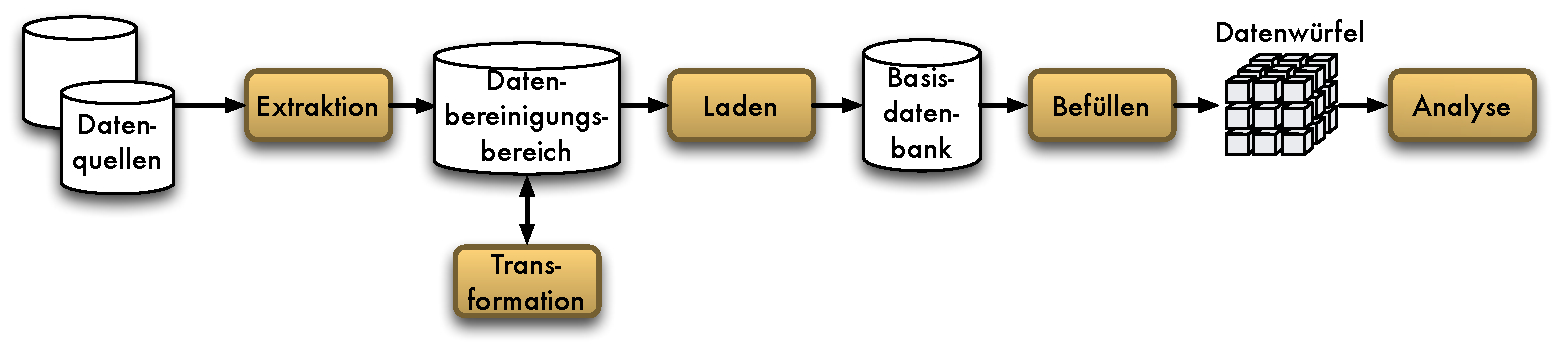
\includegraphics[width=.99\textwidth]{fig6/Referenzarchitektur-1.pdf}
        \end{center}
    
        \end{frame}
        %--------------------------------------------------------------
    
    \begin{frame}[c]
        \frametitle{Beispiel einer Anfrage}
    
        \begin{beamercolorbox}[sep=4pt,colsep*=5pt,shadow=true,rounded=false]{sqlexample}%
        \begin{quote}
            Welche \hl{Umsätze} sind in den \hl{Jahren} 2009 und 2010 in den
                \hl{Warensegmenten} Bier und Rotwein in den
                \hl{Bundesländern} Sachsen-Anhalt und Thüringen angefallen?
        \end{quote}
        \end{beamercolorbox}
    
        \end{frame}
    

    \section{Datenmodellierung}

    \frame{
      \frametitle{Überblick}
      \tableofcontents[currentsection,hidesubsections,firstsection=24]
    }


    \begin{frame}

        \frametitle{Grundbegriffe}
        \begin{itemize}
            \item Dimensionen
            \item Fakten / Kennzahlen
        \end{itemize}
        \begin{center}
        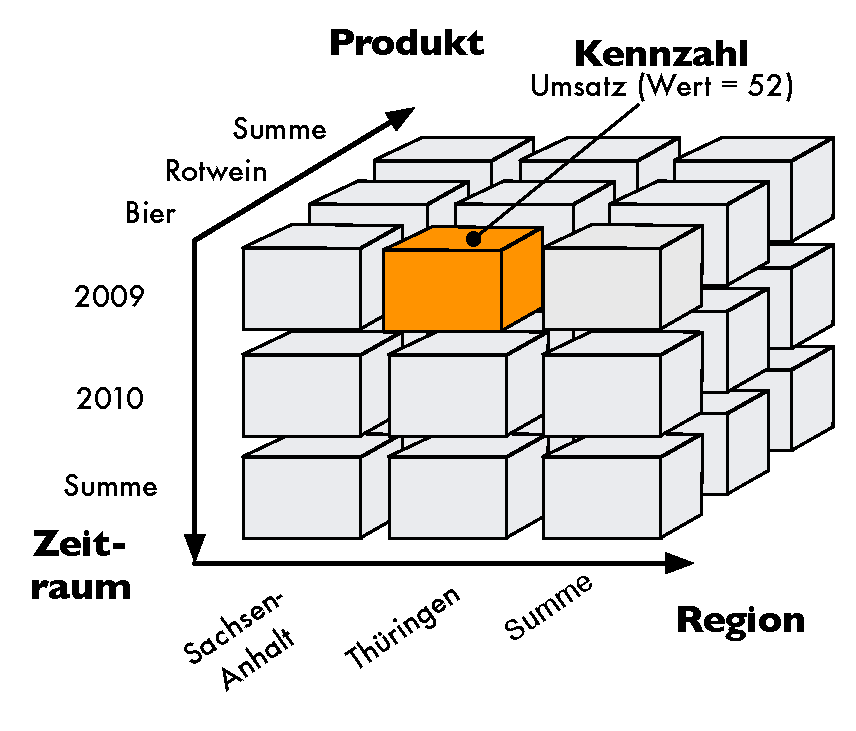
\includegraphics[height=0.8\textAreaHeight]{fig6/Wuerfel.pdf}
        \end{center}

        \end{frame}

        \begin{frame}

        \frametitle{Motivation}
        \begin{itemize}
        \item Datenmodell ausgerichtet auf Unterstützung der Analyse
        \item Datenanalyse im Entscheidungsprozess
          \begin{itemize}
          \item Betriebswirtschaftliche Kennzahlen  stehen im Mittelpunkt\\ $\to$ \hl{Fakten}

            $\bullet$ Gewinn, $\bullet$ Umsatz, $\bullet$ Kosten, $\bullet$ etc.
          \item Betrachtung der Kennzahlen aus unterschiedlichen Perspektiven\\ $\to$ \hl{Dimensionen}

            $\bullet$  Zeit, $\bullet$  Raum, $\bullet$  Sache
          \item Unterteilung der Auswertedimensionen möglich\\ $\to$ \hl{Hierarchien} oder
            \hl{Konsolidierungsebenen}

          $\bullet$  Jahr, $\bullet$  Quartal, $\bullet$  Monat
        \end{itemize}
        \end{itemize}
        \end{frame}

        %%%%%%%%%%%%%%%%%%%%%%%%%%%%%%%%%%%%%%%%%%%%%%%%%%%%%%%%%%%%%%%%%%%%%%%%
        \begin{frame}

        \frametitle{Verfügbare Informationen}

        \begin{itemize}
        \item Qualifizierend
        \begin{itemize}
        \item Repräsentiert durch "`Kategorienattribute"'
        \item Daten zur Nutzung als Navigationsraster ("`Drill-Pfade"')
        \item Modelliert als Begriffshierarchien im Rahmen von Dimensionen
        \end{itemize}
        \item Quantifizierend
        \begin{itemize}
        \item Bilden Gegenstand der Auswertung \\
        ("`Summenattribute"' oder andere arithmetische Operationen)
        \item Zellen eines Würfels, mit Dimensionen als Kanten
        \end{itemize}
        \end{itemize}

        \end{frame}

        %%%%%%%%%%%%%%%%%%%%%%%%

        \begin{frame}

        \frametitle{Dimensionen}
        \begin{itemize}
        \item Dimension:
        \begin{itemize}
        \item Beschreibt mögliche Sicht auf assoziierte Kennzahlen
        \item Endliche Menge von $n$ ($n \geq 2$) Dimensionselementen
          (Hierarchieobjekten), die eine semantische Beziehung aufweisen
        \item Dienen der orthogonalen Strukturierung des Datenraums
        \end{itemize}
        \item Beispiele:
        \begin{itemize}
            \item Produkt,
            \item Filialstruktur,
            \item Geschäftsjahr
        \end{itemize}
        \end{itemize}

        \end{frame}

        %%%%%%%%%%%%%%%%%%%%%%%%
        \begin{frame}

        \frametitle{Hierarchien in Dimensionen}
        \begin{itemize}
        \item Dimensionselemente:
        \begin{itemize}
        \item Knoten einer Klassifikationshierarchie
        \item Klassifikationsstufe beschreibt Verdichtungsgrad
        \item Darstellung von Dimensionen über Klassifikationsschema (Schema
          von Klassifikationshierarchien)
        \end{itemize}
        \item Formen:
        \begin{itemize}
        \item Einfache Hierarchien
        \item Parallele Hierarchien
        \end{itemize}
        \end{itemize}
        \end{frame}

        %%%%%%%%%%%%%%%%%%%%%%%%
        \begin{frame}

        \frametitle{Einfache Hierarchie}
        \begin{itemize}
        \item Höhere Hierarchieebene enthält die aggregierten Werte genau
          einer niedrigeren Hierarchiestufe
        \item Oberster Knoten: $Top$
          \begin{itemize}
          \item
            Enthält Verdichtung auf einen einzelnen Wert für die Dimension
          \end{itemize}
        \end{itemize}

        \begin{center}
        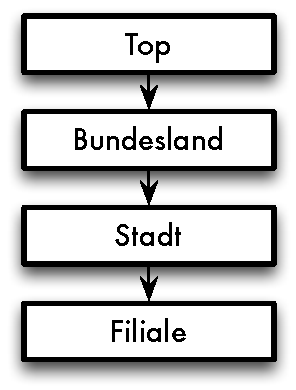
\includegraphics[scale=.46]{fig6/Einfache-Hierarchien.pdf}
        \end{center}
        \end{frame}

        %%%%%%%%%%%%%%%%%%%%%%%%
        \begin{frame}

        \frametitle{Parallele Hierarchie}

        \begin{itemize}
        \item Innerhalb einer Dimension sind mehrere unabhängige Arten der
          Gruppierung möglich
        \item Keine hierarchische Beziehung zwischen parallelen Zweigen
        \item Parallelhierarchie: $\bullet$ Pfad im Klassifikationsschema $\bullet$ Konsolidierungspfad

        \end{itemize}

        \begin{center}
        %\hspace{5cm}
        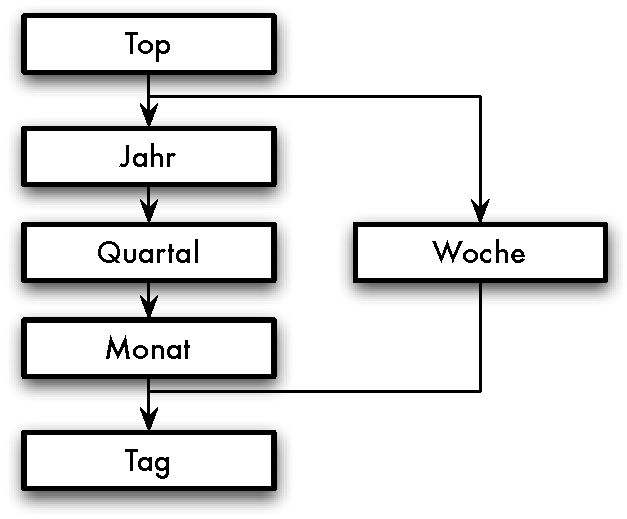
\includegraphics[height=0.46\textAreaHeight]{fig6/Parallele-Hierarchien.pdf}
        \end{center}

        \end{frame}

        %%%%%%%%%%%%%%%%%%%%%%%%


        \begin{frame}

        \frametitle{Kategorienattribute}
        \begin{itemize}
        \item Inhaltliche Verfeinerung durch unterschiedliche Rollen:
        \item Primärattribut
          \begin{itemize}
          \item Kategorienattribut, das alle anderen Attribute einer Dimension
            bestimmt
          \item Definiert maximale Feinheit
          \item Beispiel: "`Auftragsposition"'
        \end{itemize}
        \item Klassifikationsattribut
          \begin{itemize}
          \item Element der Menge, die mehrstufige Kategorisierung
            (Klassifikationshierarchie) bilden
          \item Beispiel: "`Produkt"', "`Produktgruppe"', "`Produktkategorie"'
        \end{itemize}
        \item Dimensionales Attribut
          \begin{itemize}
          \item Element der Menge der Attribute, die vom Primärattribut oder
            einem Klassifikationsattribut bestimmt werden und nur $Top_D$
            bestimmen
          \item Beispiel: "`Regalposition"'
        \end{itemize}
        \end{itemize}

        \end{frame}

        %%%%%%%%%%%%%%%%%%%%%%%%
        \begin{frame}

        \frametitle{Struktur einer Dimension: Beispiel}

        \begin{center}
        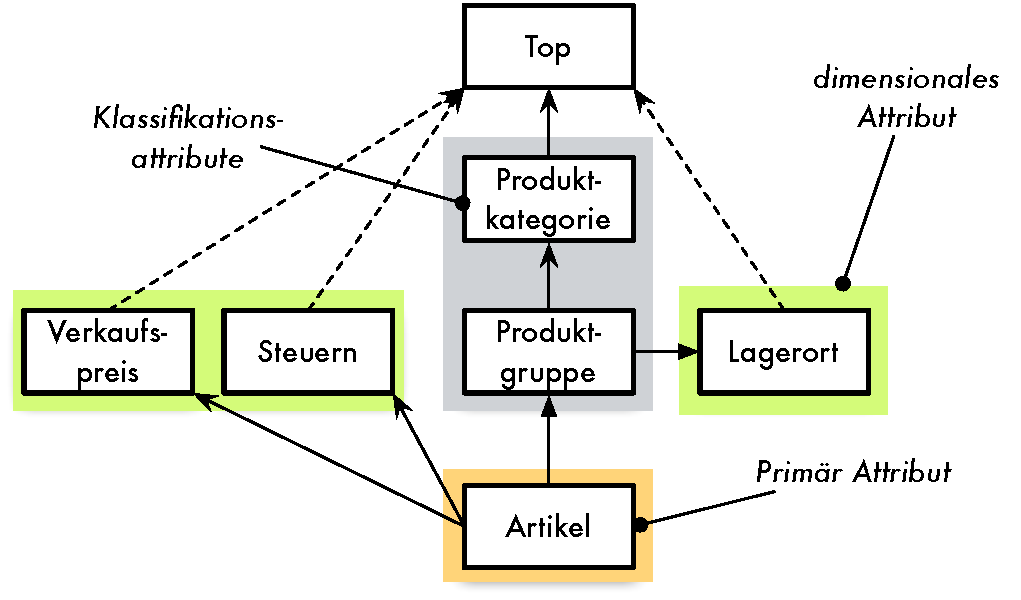
\includegraphics[scale=.6]{fig6/Dimensionsstruktur.pdf}
        \end{center}
        \end{frame}

        %%%%%%%%%%%%%%%%%%%%%%%%
        \begin{frame}

        \frametitle{Kennzahlen}
        \begin{itemize}
        \item Kennzahlen / Fakten (engl. \emph{facts}):
          \begin{itemize}
          \item (Verdichtete) numerische Messgrößen
          \item Beschreiben betriebswirtschaftliche Sachverhalte
          \end{itemize}
        \item \hl{Fakt}: Maßzahl (engl. \emph{measure})
        \item \hl{Kennzahl}:
          \begin{itemize}
          \item Aus Fakten konstruiert (abgeleitete Kennzahl)
          \item Durch Anwendung arithmetischer Operationen
          \end{itemize}
        \item  Beispiele:
          \begin{itemize}
          \item Umsatz, Gewinn, Kosten
          \item Deckungsbeitrag, ROI (Return on Investment)
          \item Fluktuationsquote, Umsatzsteigerung
          \end{itemize}
        \end{itemize}

        \end{frame}

        %%%%%%%%%%%%%%%%%%%%%%%%

        \begin{frame}

          \frametitle{Fakt: Schema}
        %Besteht aus
          \begin{itemize}
          \item Schema wird durch mehrere  Bestandteile spezifiziert
          \item \hl{Granularität} $G = \{ G_1, \dots , G_k \}$
            \begin{itemize}
            \item $G$ ist Teilmenge aller Kategorienattribute aller im Schema
              existierenden Dimensionsschemata $\leadsto$ keine funktionalen Abhängigkeit zwischen Kategorienattributen
                einer Granularität
            \item "`Detailliertheitsgrad"' der Fakten
            \end{itemize}
          \item \hl{Summationstyp} $SumTyp$
          \begin{itemize}
              \item Bestandsgröße STOCK
              \item Stromgröße FLOW
              \item Einheit VALUE-PER-UNIT
            \end{itemize}
          \end{itemize}


        \end{frame}

        %%%%%%%%%%%%%%%%%%%%%%%%

        \begin{frame}

        \frametitle{Kennzahl}
        \begin{itemize}
        \item \hl{Kennzahl} $M$ ist definiert durch
        \begin{itemize}
        \item Granularität $G$
        \item Berechnungsvorschrift $f()$ über Fakten
        \item Summationstyp $SumTyp$
        \end{itemize}
        \item Berechnung über nichtleerer Teilmenge der im Schema
          existierenden Fakten
        \end{itemize}

        \end{frame}

        %%%%%%%%%%%%%%%%%%%%%%%%

        \begin{frame}

        \frametitle{Kennzahl: Bildung von f()}
        \begin{itemize}
        \item Skalarfunktionen
          \begin{itemize}
          \item $+, -, *, /, mod$
          \item Beispiel: $Umsatzsteueranteil = Menge * Preis * Steuersatz$
          \end{itemize}
        \item Aggregatfunktionen
          \begin{itemize}
          \item Funktion $H()$ zur Verdichtung eines Datenbestandes, indem aus
            $n$ Einzelwerten ein Aggregatwert ermittelt wird
        $$ H: 2 ^{dom(X_1) \times \cdots \times  dom(X_n)} \to dom(Y)$$
        \item Bsp.: $SUM(), AVG(), MIN(), MAX(), COUNT()$
        \end{itemize}
        \item Ordnungsbasierte Funktionen
          \begin{itemize}
          \item Definition von Kennzahlen auf Basis zuvor definierter
            Ordnungen
          \item Bsp.: Kumulation, $TOP(n)$, $MEDIAN()$
          \end{itemize}
        \end{itemize}

        \end{frame}

        %%%%%%%%%%%%%%%%%%%%%%%%
        \begin{frame}

        \frametitle{Summationstypen}
        \begin{itemize}
        \item Zuweisung eines \hl{Summationstyps} charakterisiert erlaubte
          Aggregationsoperationen
        \item Stromgröße (FLOW)
          \begin{itemize}
          \item zeitraumbezogen (pro Zeiteinheit)
          \item Beliebig aggregierbar
          \item Beispiel: Bestellmenge eines Artikels pro Tag
          \end{itemize}
        \item Bestandsgröße (STOCK)
          \begin{itemize}
          \item Maß über Zeitraum
          \item Beliebig aggregierbar mit Ausnahme temporaler Dimension
          \item Beispiel: Lagerbestand, Einwohnerzahl
          \end{itemize}
        \item Einheit (VALUE-PER-UNIT - VPU)
          \begin{itemize}
          \item zeitpunktbezogen (zum Zeitpunkt)
          \item Aktuelle Zustände, die nicht summierbar sind
          \item Zulässig nur: $MIN(), MAX(), AVG()$
          \item Beispiele: Preis, Wechselkurs, Steuersatz
        \end{itemize}
        \end{itemize}

        \end{frame}

        %%%%%%%%%%%%%%%%%%%%%%%%
        \begin{frame}

        \frametitle{Summierbarkeit}

        \begin{center}

                \begin{tabular}{|c|c|c|c|c|}
                \hline &	FLOW	& \multicolumn{2}{c|}{STOCK} & 	VPU \\
                \hline  && \multicolumn{2}{c|}{Aggregation	über} &\\
                && \multicolumn{2}{c|}{temporale Dimension?}	& \\
                  \cline{3-4}		&&	nein&	ja&	\\
                \hline	\hline $MIN/MAX$	&$+$	&\multicolumn{2}{c|}{$+$}		&$+$\\
                \hline	$SUM$	&$+$	&$+$&	$-$&	$-$\\
                \hline	$AVG$	&$+$&\multicolumn{2}{c|}{$+$}	&	$+$\\
                \hline	$COUNT$	&$+$	&\multicolumn{2}{c|}{$+$}	&$	+$\\
                \hline
                \end{tabular}
        \end{center}

        \end{frame}

        %%%%%%%%%%%%%%%%%%%%%%%%

\section{Relationale Speicherung}


        \begin{frame}

            \frametitle{Relationale Speicherung}
            \begin{itemize}
            \item Vermeidung des Verlustes anwendungsbezogener Semantik (aus dem
              multidimensionalen Modell, z.B. Klassifikationshierarchien)
            \item Effiziente Übersetzung multidimensionaler Anfragen
            \item Effiziente Verarbeitung der übersetzten Anfragen
            \item Einfache Pflege der entstandenen Relationen (z.B. Laden neuer
              Daten)
            \item Berücksichtigung der Anfragecharakteristik und des Datenvolumens
              von Analyseanwendungen
            \end{itemize}
        
            \end{frame}
        
            %%%%%%%%%%%%%%%%%%%%%%%%%%%%%%%%%%%%%%%%%%%%%%%%%%%%%%%%%%%%%%%%%%%%%%%%
        
            \begin{frame}
        
            \frametitle{Relationale Umsetzung: Faktentabelle}
            \begin{itemize}
            \item Ausgangspunkt: Umsetzung des Datenwürfels ohne
              Klassifikationshierarchien
              \begin{itemize}
              \item Dimensionen, Kennzahlen $\to$ Spalten der Relation
              \item Zelle $\to$ Tupel
              \end{itemize}
            \end{itemize}
        
            \begin{columns}[c]
            \begin{column}{3.5cm}
              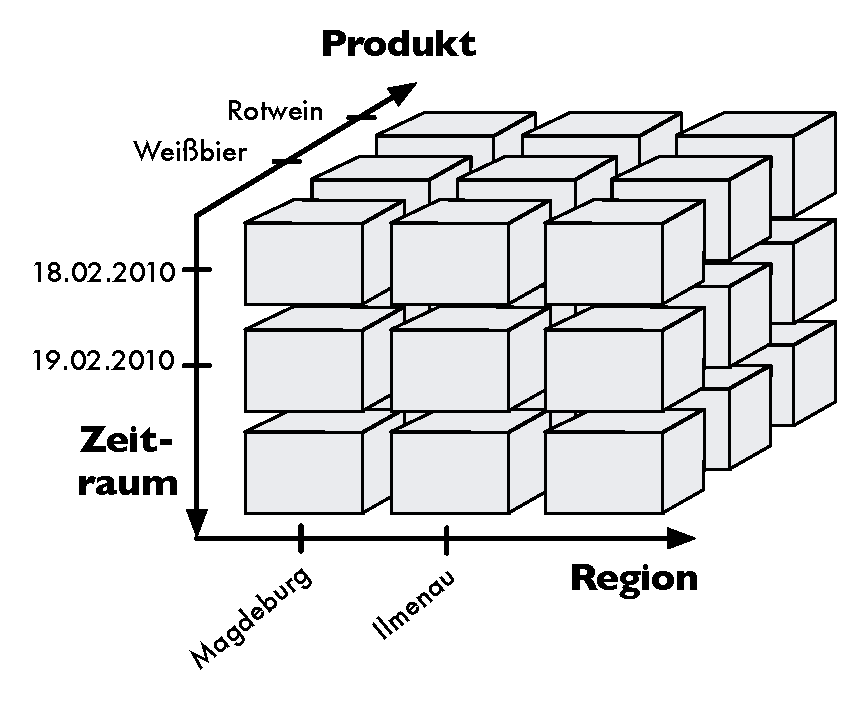
\includegraphics[width = 1.3\textwidth]{fig6/Faktentabelle.pdf}
            \end{column}
            \begin{column}{5cm}
            {\scriptsize
            \begin{tabular}{|l|l|l|c|}
            \hline
            \rowcolor{Gray}  Produkt & Filiale & Tag & Verk. \\
            \hline
            \hline
            Rotwein & Magdeburg & 18.02.10 & 145 \\
            Weißbier & Magdeburg & 18.02.10 & 267 \\
            Rotwein & Ilmenau & 18.02.10 & 70 \\
            \multicolumn{4}{|c|}{\dots}\\
            \hline
            \end{tabular}
            }
            \end{column}
            \end{columns}
            \end{frame}
        
            %%%%%%%%%%%%%%%%%%%%%%%%%%%%%%%%%%%%%%%%%%%%
            \begin{frame}
        
            \frametitle{Snowflake-Schema}
        
            \begin{itemize}
            \item Abbildung von Klassifikationen: eigene Tabelle für jede
              Klassifikationsstufe (z.B. Artikel, Produktgruppe, etc.)
            \item Dimensionstabelle enthält
              \begin{itemize}
              \item ID für Klassifikationsknoten
              \item Beschreibendes Attribut (z.B. Marke, Hersteller, Bezeichnung)
              \item Fremdschlüssel der direkt übergeordneten Klassifikationsstufe
              \end{itemize}
            \item Faktentabelle enthält (neben Kenngrößen):
              \begin{itemize}
              \item Fremdschlüssel der jeweils niedrigsten Klassifikationsstufe
              \item Fremdschlüssel bilden zusammengesetzte Primärschlüssel für
                Faktentabelle
              \end{itemize}
            \end{itemize}
        
            \end{frame}
        
            %%%%%%%%%%%%%%%%%%%%%%%%%%%%%%%%%%%%%%%%%%%%
            \begin{frame}
        
            \frametitle{Snowflake-Schema: Muster}
        
            \begin{center}
              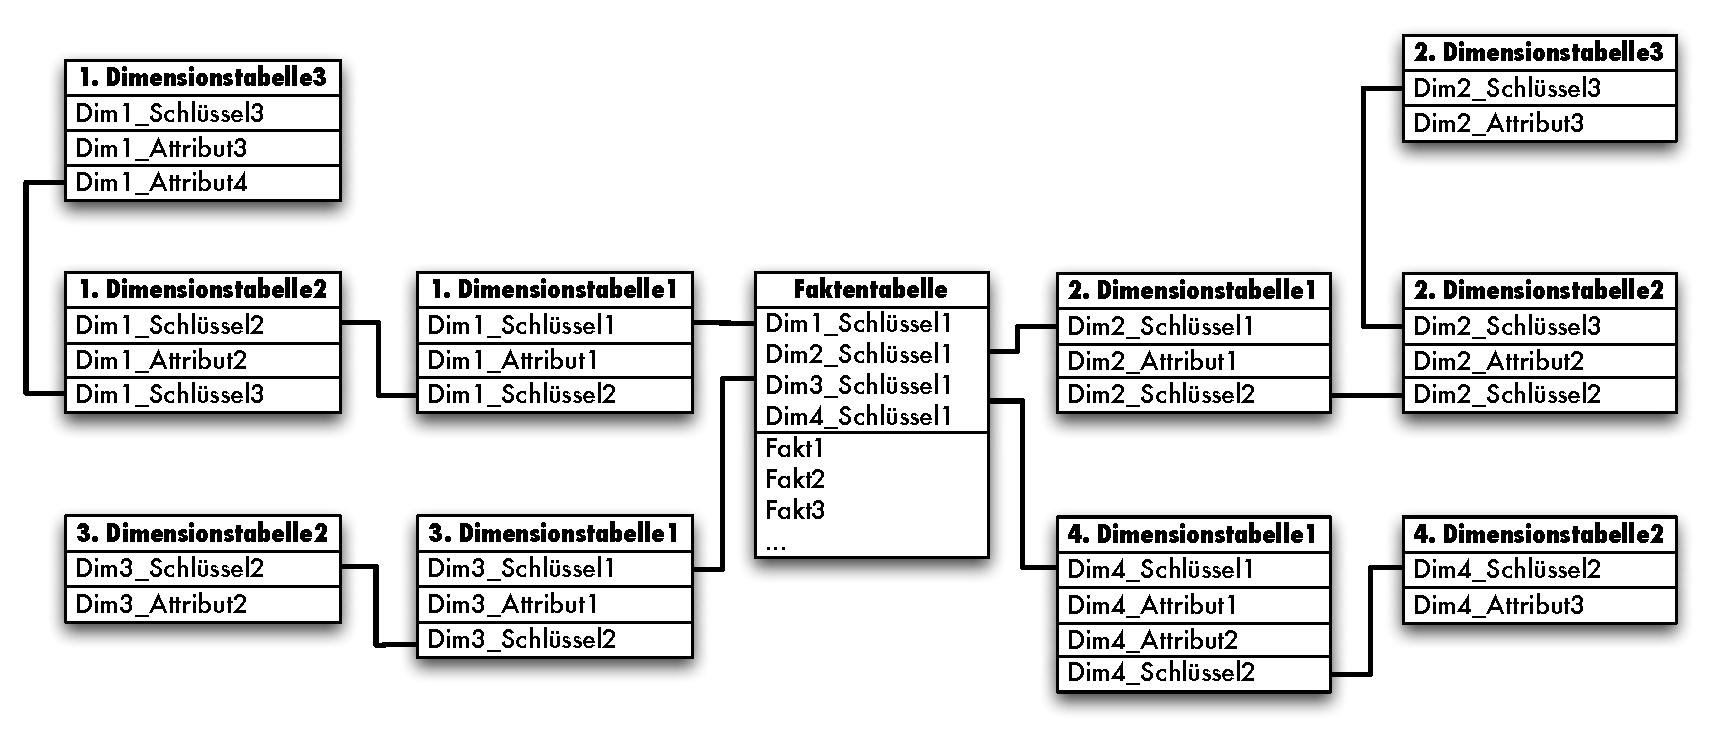
\includegraphics[width=\textwidth]{fig6/Snowflake-Schema.pdf}
            \end{center}
        
            \end{frame}
            %%%%%%%%%%%%%%%%%%%%%%%%%%%%%%%%%%%%%%%%%%%%
            \begin{frame}
        
            \frametitle{Snowflake-Schema: Beispiel}
        
            \begin{center}
              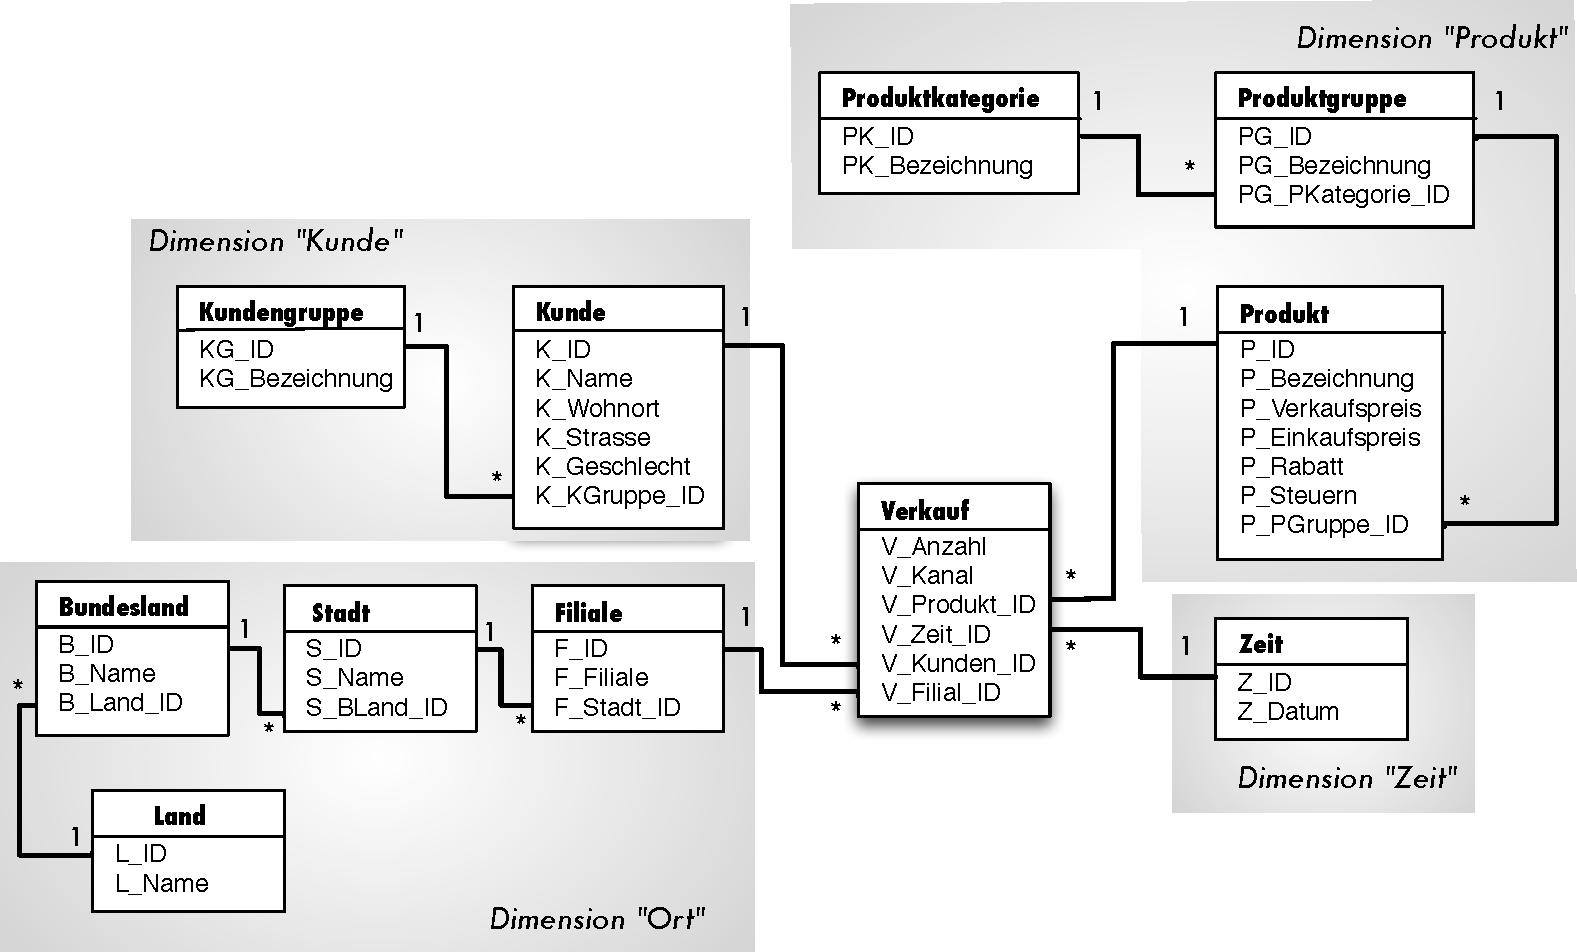
\includegraphics[height=\textAreaHeight,width=\textwidth,keepaspectratio]{fig6/SnowflakeSchema-Buch.pdf}
            \end{center}
        
            \end{frame}
        
            %%%%%%%%%%%%%%%%%%%%%%%%%%%%%%%%%%%%%%%%%%%%
        
            \begin{frame}
        
            \frametitle{Star-Schema}
        
            \begin{itemize}
            \item Snowflake-Schema ist normalisiert: Vermeidung von
              Update-Anomalien $\to$ \hl{3. NF}
              \begin{itemize}
              \item Aber: erfordert Join über mehrere Tabellen!
              \end{itemize}
            \item Star-Schema:
              \begin{itemize}
              \item Denormalisierung der zu einer Dimension gehörenden Tabellen $\to$ \hl{1. NF}
              \item Für jede Dimension genau eine Dimensionstabelle
              \item Redundanzen in der Dimensionstabelle für schnellere
                Anfragebearbeitung
              \item Beispiel: Artikel, Produkt, Produktgruppe etc. als Spalten in
                einer Tabelle Produkt
              \end{itemize}
            \end{itemize}
        
            \end{frame}
        
            %%%%%%%%%%%%%%%%%%%%%%%%%%%%%%%%%%%%%%%%%%%%
        
            \begin{frame}
        
            \frametitle{Star-Schema: Muster}
        
            \begin{center}
              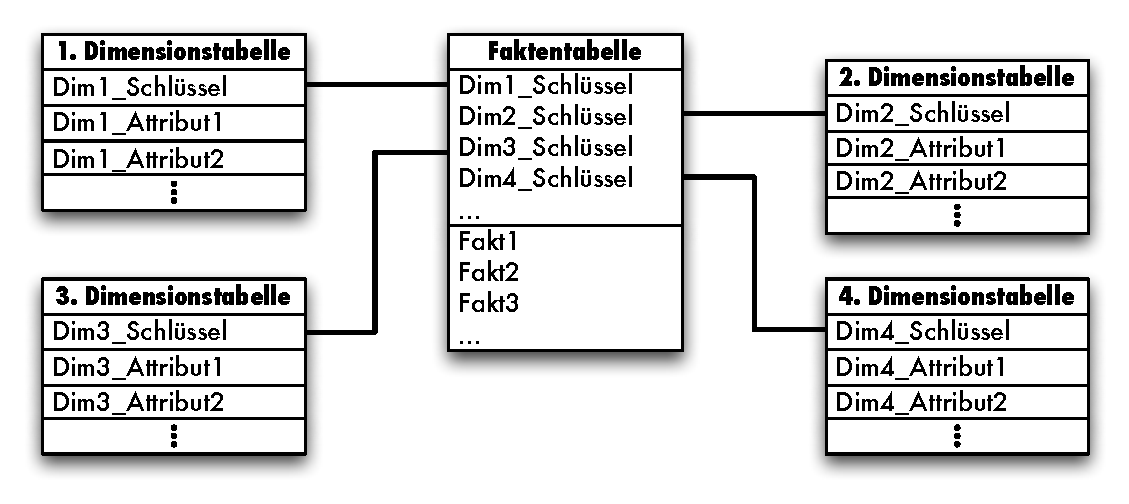
\includegraphics[scale=.6]{fig6/StarSchema.pdf}
            \end{center}
        
            \end{frame}
        
            %%%%%%%%%%%%%%%%%%%%%%%%%%%%%%%%%%%%%%%%%%%%
        
        
            \begin{frame}
        
            \frametitle{Star-Schema: Beispiel}
        
            \begin{center}
              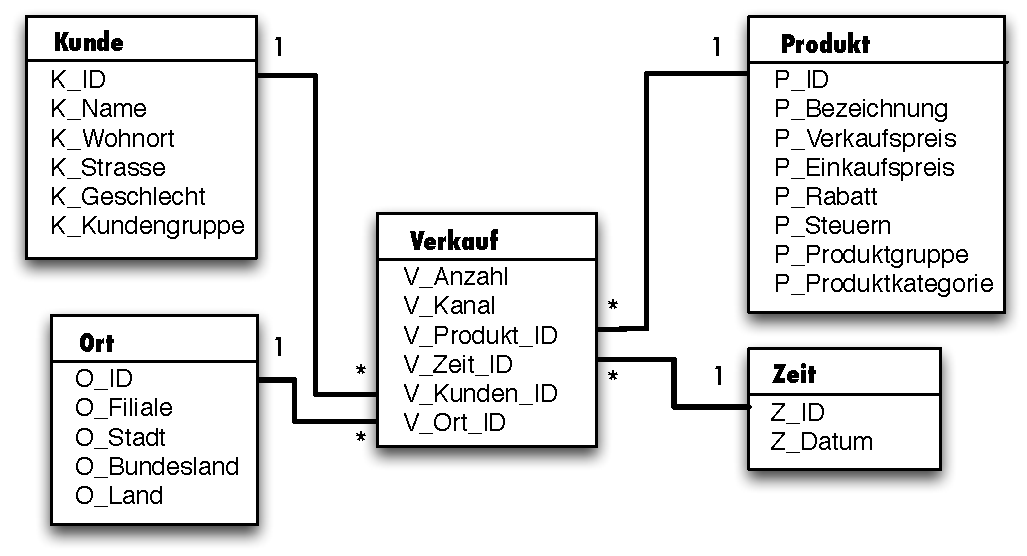
\includegraphics[height=\textAreaHeight,width=\textwidth,keepaspectratio]{fig6/Star-Schema.pdf}
            \end{center}
        
        
            \end{frame}
        
            %%%%%%%%%%%%%%%%%%%%%%%%%%%%%%%%%%%%%%%%%%%%
            \begin{frame}
        
            \frametitle{Star-Schema formal}
        
            \begin{itemize}
            \item Multidimensionales Schema mit $n$ Dimensionen
              \begin{itemize}
              \item Dimensionstabellen $D^1, \dots, D^n$ der Form $D^i(Dim_i\_Key,
                A_{i,1}, \dots, A_{i,{k_i}})$
              \item Faktentabelle $F(Dim_1\_Key, \dots, Dim_n\_Key, f_1, \dots, f_m)$ mit $m$ Fakten
              \end{itemize}
            \item Jeder Teil des kompositen Primärschlüssels der Faktentabelle ist
              Fremdschlüssel zum Primärschlüsselattribut der korrespondierenden
              Dimension
            \end{itemize}
        
            \end{frame}
        
            \begin{frame}
        
                \frametitle{Mischformen}
        
                \begin{itemize}
                \item Abbildung einzelner Dimensionen analog Snowflake-Schema oder
                  Star-Schema
                \item Entscheidungskriterien:
                  \begin{itemize}
                  \item Änderungshäufigkeit der Dimensionen:
                    \begin{itemize}
                    \item Reduzierung des Pflegeaufwandes durch Normalisierung
                      (Snowflake)
                    \end{itemize}
                  \item Anzahl der Klassifikationsstufen einer Dimension:
                    \begin{itemize}
                    \item Mehr Klassifikationsstufen $\to$ größere Redundanz im
                      Star-Schema
                    \end{itemize}
        
                  \item Anzahl der Dimensionselemente:
                    \begin{itemize}
                    \item Einsparung durch Normalisierung bei vielen Elementen einer
                      Dimension auf niedrigster Klassifikationsstufe
                    \end{itemize}
                  \item Materialisierung von Aggregaten:
                    \begin{itemize}
                    \item Performance-Verbesserung durch Normalisierung bei
                      materialisierten Aggregaten für eine Klassifikationsstufe
                    \end{itemize}
                  \end{itemize}
                \end{itemize}
        
                \end{frame}
        
        
                %%%%%%%%%%%%%%%%%%%%%%%%%%%%%%%%%%%%%%%%%%%%
                \begin{frame}
        
                \frametitle{Galaxie-Schema}
        
        
                \begin{itemize}
                \item Star- und Snowflakeschema
                  \begin{itemize}
                  \item Eine Faktentabelle
                  \item Mehrere Kennzahlen nur möglich bei gleichen Dimensionen
                  \end{itemize}
                \item Galaxie-Schema
                  \begin{itemize}
                  \item Mehrere Faktentabellen
                  \item Teilweise mit gleichen Dimensionstabellen verknüpft
                  \item Auch: Multi-Faktentabellen-Schema, Multi-Cube, Hyper-Cube
                  \end{itemize}
                \end{itemize}
        
                \end{frame}
        
                %%%%%%%%%%%%%%%%%%%%%%%%%%%%%%%%%%%%%%%%%%%%
                \begin{frame}
        
                \frametitle{Galaxie-Schema: Muster}
        
                \begin{center}
                  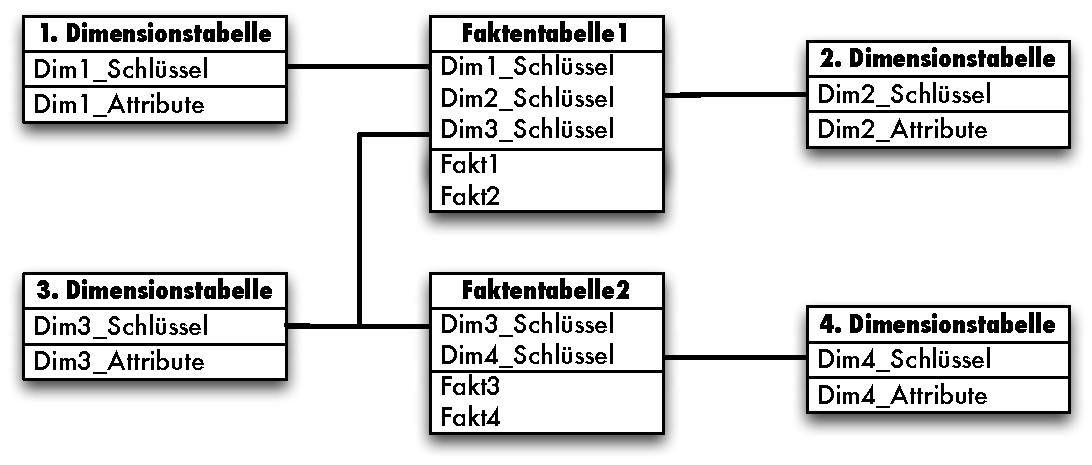
\includegraphics[width=\textwidth]{fig6/Galaxy-Schema.pdf}
                \end{center}
        
                \end{frame}
                %%%%%%%%%%%%%%%%%%%%%%%%%%%%%%%%%%%%%%%%%%%%
        
                \begin{frame}
        
                \frametitle{Galaxie-Schema: Beispiel}
        
                \begin{center}
                  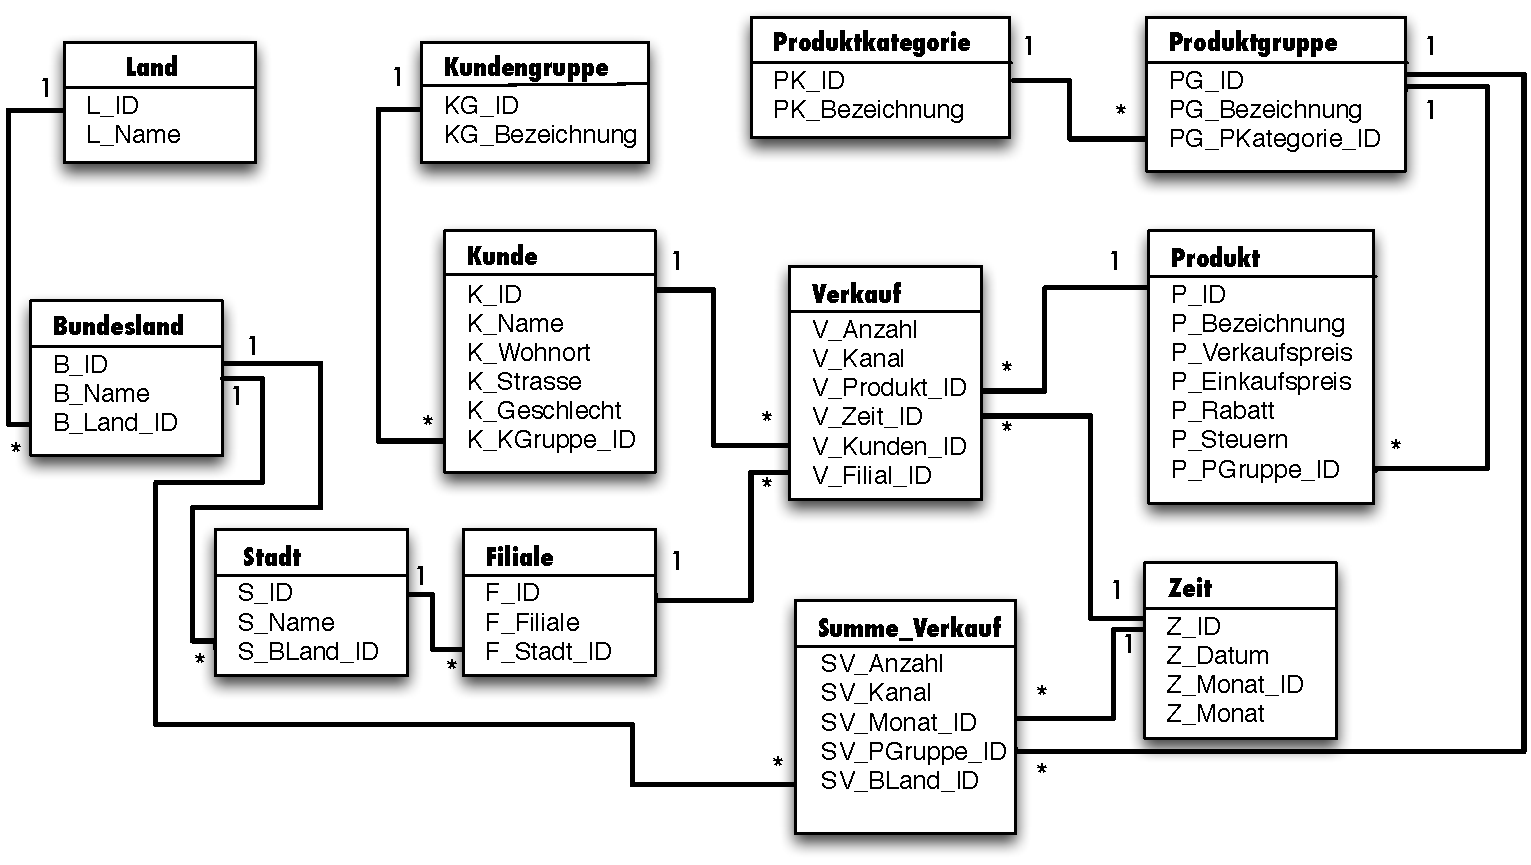
\includegraphics[height=\textAreaHeight,width=\textwidth,keepaspectratio]{fig6/GalaxySchema-Beispiel.pdf}
                \end{center}
        
                \end{frame}
                %%%%%%%%%%%%%%%%%%%%%%%%%%%%%%%%%%%%%%%%%%%%
        
                \begin{frame}
        
                \frametitle{Fact Constellation}
                \begin{itemize}
                \item Speicherung vorberechneter Aggregate in Faktentabelle
                  \begin{itemize}
                  \item Beispiel: Umsatz für Region
                  \item Unterscheidung in Dimensionstabelle über spezielle Attribute
                    (Bsp.: "`Stufe"')
                  \end{itemize}
                \item Alternative: Auslagerung in eigene Faktentabelle
                  \begin{itemize}
                  \item Fact-Constellation-Schema (Spezialfall eines Galaxie-Schemas)
                  \end{itemize}
                \end{itemize}
        
                \end{frame}
        
                %%%%%%%%%%%%%%%%%%%%%%%%%%%%%%%%%%%%%%%%%%%%
        
        
        
                \begin{frame}
        
                \frametitle{Fact Constellation: Beispiel}
        
                \begin{center}
                  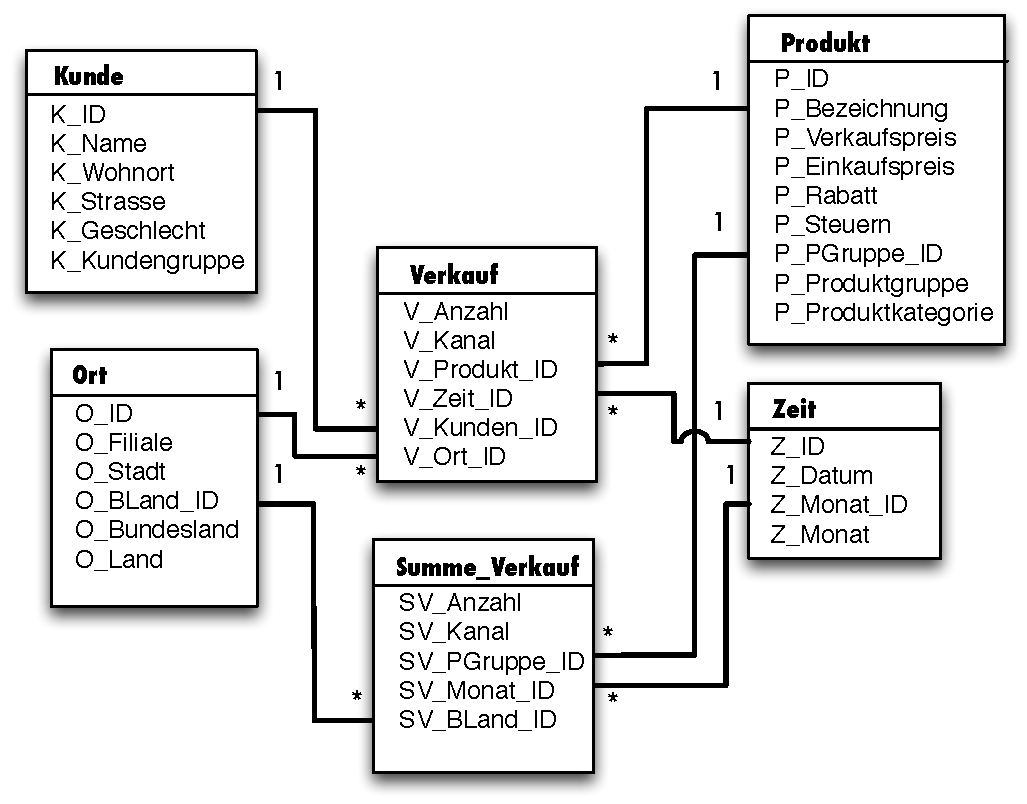
\includegraphics[height=\textAreaHeight]{fig6/Fact-Constellation-Schema.pdf}
                \end{center}
        
        
                \end{frame}
        
        
        \section{OLAP-Operationen zur Datenanalyse}
        
        
        \frame{
          \frametitle{Überblick}
          \tableofcontents[currentsection,hidesubsections,firstsection=24]
        }
        
        \begin{frame}
        
        \frametitle{Operationen zur Datenanalyse}
        \begin{itemize}
        \item OLAP-Operationen auf multidimensionalen Datenstrukturen
        \item Standardoperationen
          \begin{itemize}
          \item Pivotierung
          \item Roll-Up, Drill-Down
          \item Drill-Across
          \item Slice und Dice
          \end{itemize}
        \end{itemize}
        
        
        \end{frame}
        
        %%%%%%%%%%%%%%%%%%%%%%%%
        
        \begin{frame}
        
        \frametitle{Pivotierung / Rotation}
        \begin{itemize}
        \item Drehen des Würfels durch Vertauschen der Dimensionen
        \item Analyse der Daten aus verschiedenen Perspektiven
        \end{itemize}
        
        \begin{center}
        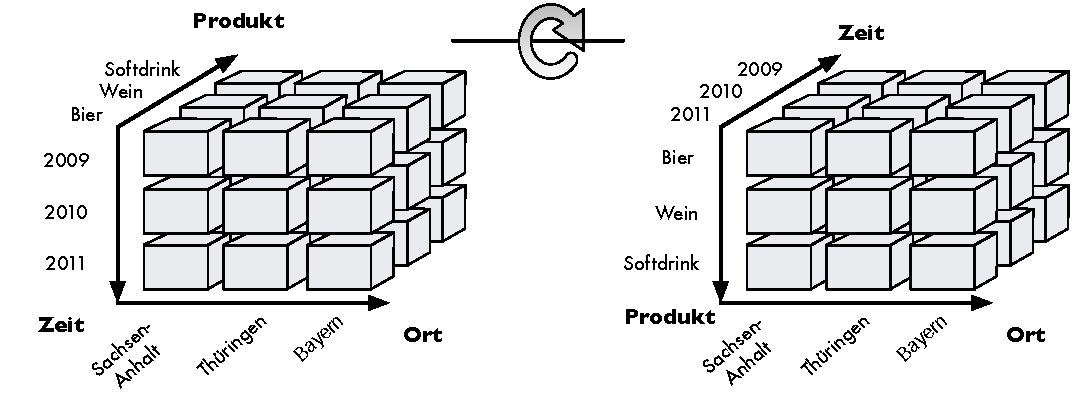
\includegraphics[scale=.6]{fig6/OLAP-Pivot.pdf}
        \end{center}
        \end{frame}
        
        %%%%%%%%%%%%%%%%%%%%%%%%
        
        \begin{frame}
        
        \frametitle{Roll-Up, Drill-Down, Drill-Across}
        \begin{itemize}
        \item \hl{Roll-Up}:
          \begin{itemize}
          \item Erzeugen neuer Informationen durch Aggregierung der Daten
            entlang des Konsolidierungspfades
          \item Dimensionalität bleibt erhalten
          \item Beispiel: Tag $\to$ Monat $\to$ Quartal $\to$ Jahr
          \end{itemize}
        \item \hl{Drill-Down}:
          \begin{itemize}
          \item Komplementär zu Roll-Up
          \item Navigation von aggregierten Daten zu Detail-Daten entlang der
            Klassifikationshierarchie
          \end{itemize}
        \item \hl{Drill-Across}:
          \begin{itemize}
          \item Wechsel von einem Würfel zu einem anderen
          \end{itemize}
        \end{itemize}
        
        
        \end{frame}
        
        %%%%%%%%%%%%%%%%%%%%%%%%
        
        \begin{frame}
        
        \frametitle{Roll-Up und Drill-Down}
        
        \begin{center}
        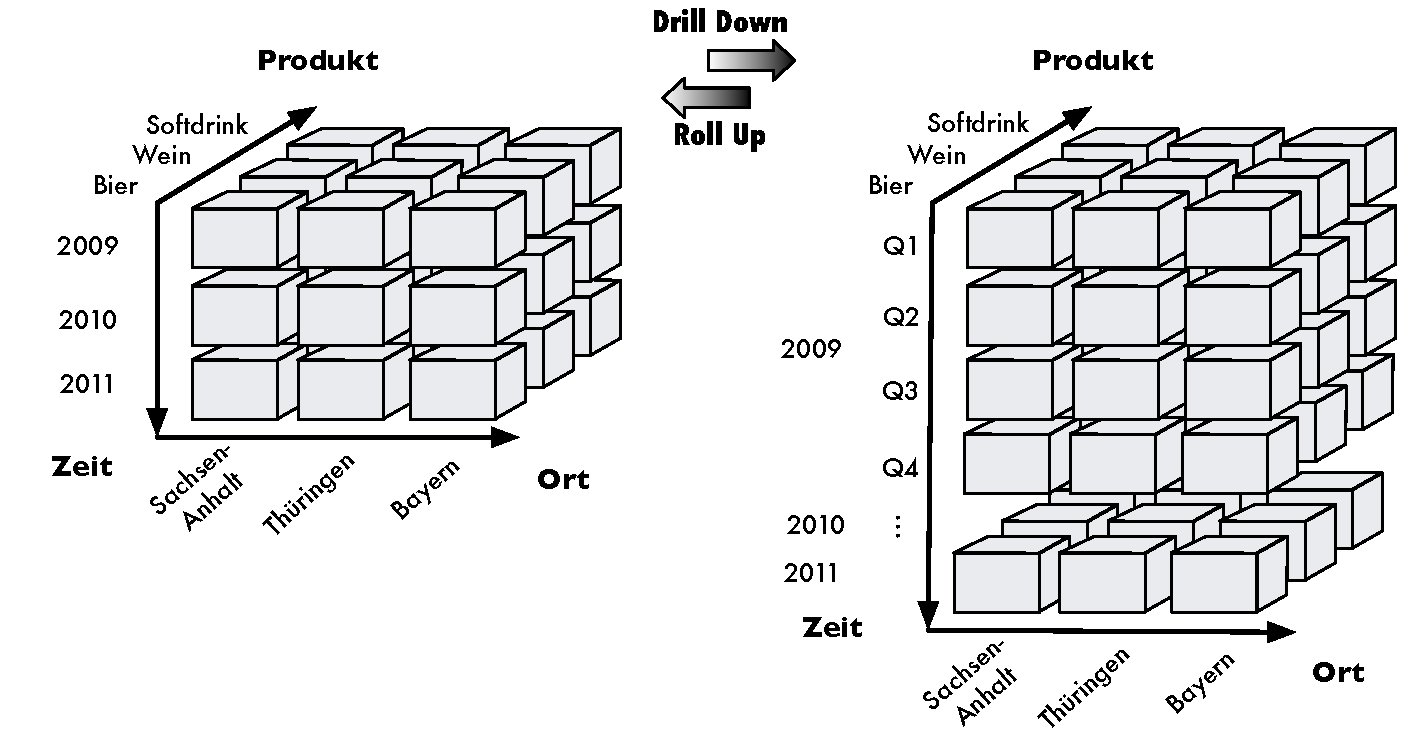
\includegraphics[scale=.46]{fig6/OLAP-DrillDown.pdf}
        \end{center}
        \end{frame}
        
        %%%%%%%%%%%%%%%%%%%%%%%%
        
        
        \begin{frame}
        
        \frametitle{Slice und Dice}
        \begin{itemize}
        \item Erzeugen individueller Sichten
        \item \hl{Slice}:
          \begin{itemize}
          \item Herausschneiden von "`Scheiben"' aus dem Würfel
          \item Verringerung der Dimensionalität durch Konditionierung der Dimensionen
          \item Beispiel: alle Werte des aktuellen Jahres
           \item \emph{Entspricht der relationalen Selektion in den Dimensionen}
          \end{itemize}
        \item \hl{Dice}:
          \begin{itemize}
          \item Herausschneiden einen "`Teilwürfels"'
          \item Erhaltung der Dimensionalität, Veränderung der
            Hierarchieobjekte
          \item Beispiel: die Werte bestimmter Produkte oder Regionen
          \item \emph{Entspricht der relationalen Selektion mehrerer Dimensionen}
        \end{itemize}
        \end{itemize}
        
        \end{frame}
        
        %%%%%%%%%%%%%%%%%%%%%%%%
        
        \begin{frame}
        
        \frametitle{Slice}
        
        \begin{center}
        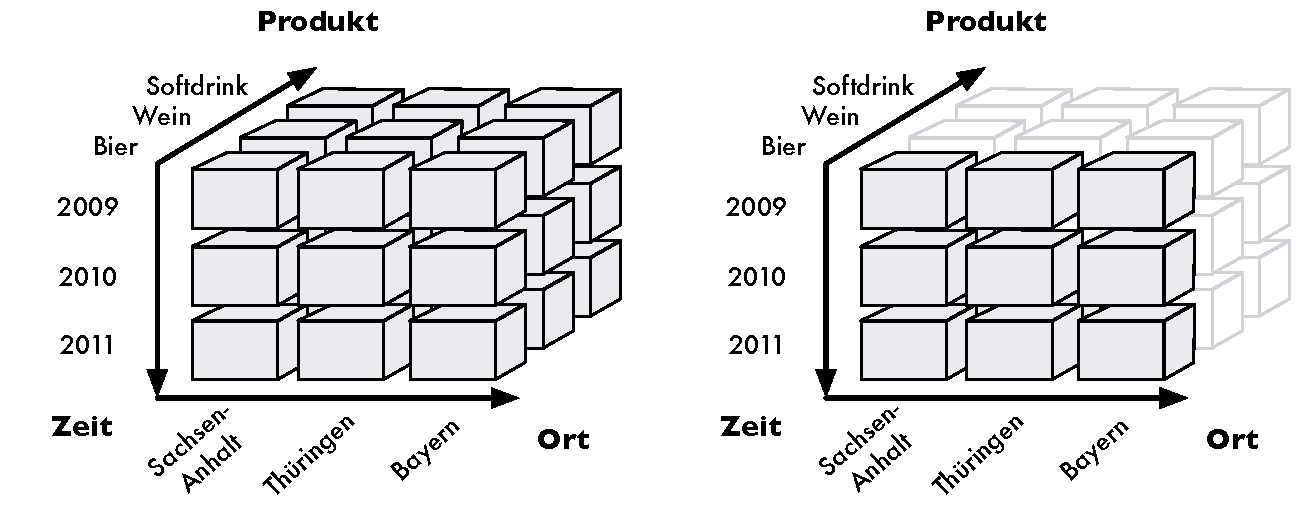
\includegraphics[width=.95\textwidth]{fig6/OLAP-Slice.pdf}
        \end{center}
        
        \end{frame}
        %%%%%%%%%%%%%%%%%%%%%%%%
        
        \begin{frame}
        
        \frametitle{Dice}
        
        \begin{center}
        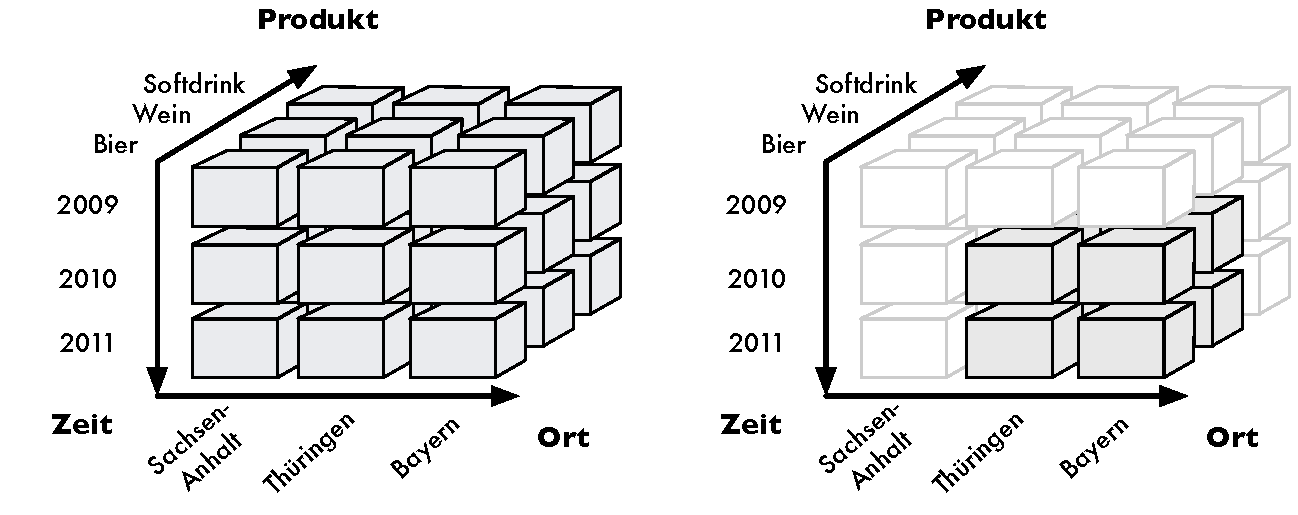
\includegraphics[width=.95\textwidth]{fig6/OLAP-Dice.pdf}
        \end{center}
        %Abbildung Slice
        
        \end{frame}
        
%-----------------------------------------------------------------------

\begin{frame}
    \frametitle{Umsetzung von OLAP-Operationen}

    \textbf{SQL}

    \begin{itemize}
        \item Star-Joins: Verbund der Faktentabelle mit den Dimensionstabellen, Gruppierung + Aggregation (siehe Teil III)
    \end{itemize}

    \textbf{Python + Pandas}

    \begin{itemize}
        \item \texttt{transpose}
        \item \texttt{groupby}, \texttt{pivot\_table}, \texttt{swaplevel}, \texttt{loc} + Indexierung
    \end{itemize}

\end{frame}  


\begin{frame}[fragile]
  \frametitle{Pandas: Pivot-Operationen}

  \begin{itemize}
    \item Daten umorganisieren (reshaping)
      \item \code{transpose}: Zeilen in Spalten umwandeln
    \end{itemize}

\begin{minted}{python}
df = pd.DataFrame({'A': [1, 2, 3, 4], 
                  'B': [10, 20, 30, 40],
                  'C': [100, 200, 300, 400]},
                  columns = ['A', 'B', 'C'])
df.transpose()
\end{minted}

{\small
\begin{center}
  \begin{tabular}{r|c|c|c|c|}
    \cline{2-5}
  & \textbf{0} & \textbf{1} & \textbf{2} & \textbf{3} \\
  \hline
  \textbf{A} &  1 & 2 & 3 & 4 \\
  \textbf{B} & 10 & 20 & 30 & 40 \\
  \textbf{C} & 100 & 200 & 300 & 400 \\
  \hline
  \end{tabular}
  \end{center}
  }
\end{frame}

\begin{frame}[fragile]
  \frametitle{Pandas: Pivot-Operationen /2}

  \begin{itemize}
      \item \code{pivot}: Konstruktion einer Pivot-Tabelle
      \begin{itemize}
      % \item zusätzlich angeben, welche Spalten im Ergebnis aufgenommen werden sollen
      \item benutzt \code{unique}-Werte der gegebenen Spalte
      \item keine Aggregationen
    \end{itemize}
    \item allgemeinere Form \code{pivot\_table}
    \end{itemize}

\end{frame}

\begin{frame}[fragile]
  \frametitle{Pandas: Pivot-Operationen /3}

  Tabelle \texttt{verkauf}

  \begin{center}
    \begin{tabular}{|c|c|c|}
    \hline
    \rowcolor{Gray} Bundesland & Jahr & Verkäufe \\
    \hline \hline
Thüringen      & 2019 &  100 \\
Thüringen      & 2020 & 105 \\
Sachsen        & 2019 & 141 \\
Sachsen        & 2020 & 143 \\
Sachsen-Anhalt & 2019 &  88 \\
Sachsen-Anhalt & 2020 &  94 \\
\hline
    \end{tabular}
  \end{center}
\end{frame}

\begin{frame}[fragile]
  \frametitle{Pandas: Pivot-Operationen /4}

  \begin{itemize}
\item Attribut \emph{Bundesland} wird ,,Index'', Attribut \emph{Verkäufe} wird aggregiert (hier summiert) 
  \end{itemize}

\begin{minted}{python}
verkauf.pivot_table(index=['Bundesland'], aggfunc='sum')
\end{minted}

\begin{center}
  \begin{tabular}{|c||c|}
  \hline
  \rowcolor{Gray}  & Verkäufe \\
  \rowcolor{Gray} Bundesland & \\
  \hline \hline
Sachsen        & 284 \\
Sachsen-Anhalt &  182 \\
Thüringen      &  205 \\
\hline 
  \end{tabular}
\end{center}

\end{frame}

\begin{frame}[fragile]
  \frametitle{Pandas: Pivot-Operationen /5}

  \begin{itemize}
\item mehrere Attribute können als Index dienen $\leadsto$ mehrdimensional
  \end{itemize}

\begin{minted}{python}
verkauf.pivot_table(index=['Bundesland', 'Jahr'], aggfunc='sum')
\end{minted}

{\small
\begin{center}
  \begin{tabular}{|c|c||c|}
  \hline
  \rowcolor{Gray}  & & Verkäufe \\
  \rowcolor{Gray} Bundesland & Jahr & \\
  \hline \hline
Sachsen        & 2019 & 141 \\
               & 2020 & 143 \\
Sachsen-Anhalt &  2019 & 88 \\
               & 2020 & 94 \\
Thüringen      &  2019 & 100 \\
               & 2020 & 105 \\
\hline 
  \end{tabular}
\end{center}
}

\end{frame}

\begin{frame}[fragile]
  \frametitle{Pandas: Gruppierung}

  \begin{itemize}
\item Gruppierung mit Aggregation ähnlich zu SQL
  \end{itemize}

\begin{minted}{python}
verkauf.groupby(['Bundesland', 'Jahr'])['Verkäufe'].sum()
\end{minted}

{\small
\begin{center}
  \begin{tabular}{|c|c||c|}
  \hline
  \rowcolor{Gray}  & &  \\
  \rowcolor{Gray} Bundesland & Jahr & \\
  \hline \hline
Sachsen        & 2019 & 141 \\
               & 2020 & 143 \\
Sachsen-Anhalt &  2019 & 88 \\
               & 2020 & 94 \\
Thüringen      &  2019 & 100 \\
               & 2020 & 105 \\
\hline 
  \end{tabular}
\end{center}
}
\end{frame}

\begin{frame}
        \frametitle{Zusammenfassung}
        
        \begin{itemize}
            \item In-Database-Analytics 
            \item Data Warehouse als Analyseplattform mit konsolidiertem und bereinigten Datenbestand
            \item Multidimensionales Datenmodell: Würfel, Kennzahlen, Dimensionen
            \item OLAP: konzeptionell, SQL, Python
        \end{itemize}
\end{frame}

%%%%%%%%%%%%%%%%%%%%%%%%%%%%%%%%%%%%%%%%%%%%%%%%%%%%%%%%%%%%%%%%%%%%%%

\part{Datenbeschaffung, -vorbereitung und -bereinigung}

\frame[plain,c]{\partpage}

\frame{
  \frametitle{Überblick}
  \tableofcontents[pausesections,hidesubsections,firstsection=15]
}

\section{Datenbeschaffung}

\frame{
  \frametitle{Überblick}
  \tableofcontents[currentsection,hidesubsections,firstsection=15]
}

    %---------------------------------------------------------------------

\section{Heterogenität und Datenfehler}

\frame{
  \frametitle{Überblick}
  \tableofcontents[currentsection,hidesubsections,firstsection=15]
}


\begin{frame}
    \frametitle{Data-Science-Prozess Revisited}
    
    \begin{center}
    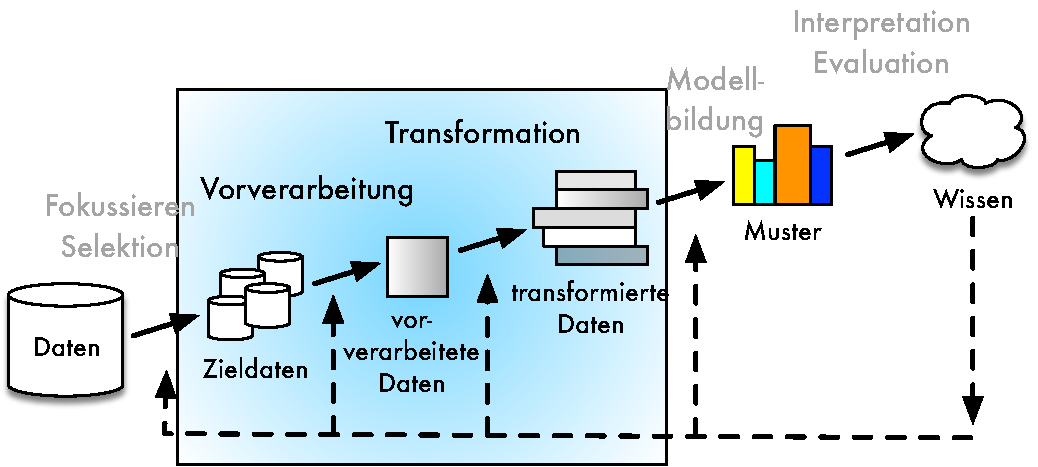
\includegraphics[scale=.6]{fig4/kdd-prozess.pdf}
    \end{center}
    
    \begin{itemize}
    \item notwendig wegen \hl{Heterogenität} durch Integration
      verschiedener Quellen und möglichen \hl{Datenfehlern}
    \end{itemize}
    
    \end{frame}
    
    %---------------------------------------------------------------------
    
    \begin{frame}
    \frametitle{Motivation: Heterogenität}
    
    \begin{itemize}
    \item \hl{verschiedene Datenmodelle}
    \begin{itemize}
    % \item bedingt durch autonome Entscheidung �ber Anschaffung von
    %   Systemen in den Unternehmensbereichen 
    \item verschiedene und verschieden mächtige Modellierungskonstrukte,
      d.h. Anwendungssemantik in unterschiedlichem Ausmaß erfassbar 
    \item Abbildung zwischen Datenmodellen nicht eindeutig
    \end{itemize}
    \item \hl{unterschiedliche Modellierungen für gleiche Sachverhalte der
        Realwelt}  
    \begin{itemize}
    \item bedingt durch Entwurfautonomie
    \item selbst im gleichen Datenmodell verschiedene Modellierungen
      möglich, z.B. durch unterschiedliche Modellierungsperspektiven 
    \end{itemize}
    \end{itemize}
    
    \end{frame}
    
    %---------------------------------------------------------------------
    
    \begin{frame}
    \frametitle{Motivation: Heterogenität /2}
    
    \begin{itemize}
    \item \hl{unterschiedliche Repräsentation der Daten}
    \begin{itemize}
    \item unterschiedliche Datentypen möglich
    \item unterschiedliche Umfang der unterstützten Datentypen
    \item unterschiedliche interne Darstellung der Daten
    \item auch unterschiedliche "`Werte"' eines Datentyps zur
      Repräsentation derselben Information 
    \end{itemize}
    \end{itemize}
    
    \end{frame}
    
    %---------------------------------------------------------------------
    
    
    \begin{frame}
    \frametitle{Datenfehler}
    
    \begin{overlayarea}{\textwidth}{5cm}
    
    \begin{center}
    \only<1| handout:0>{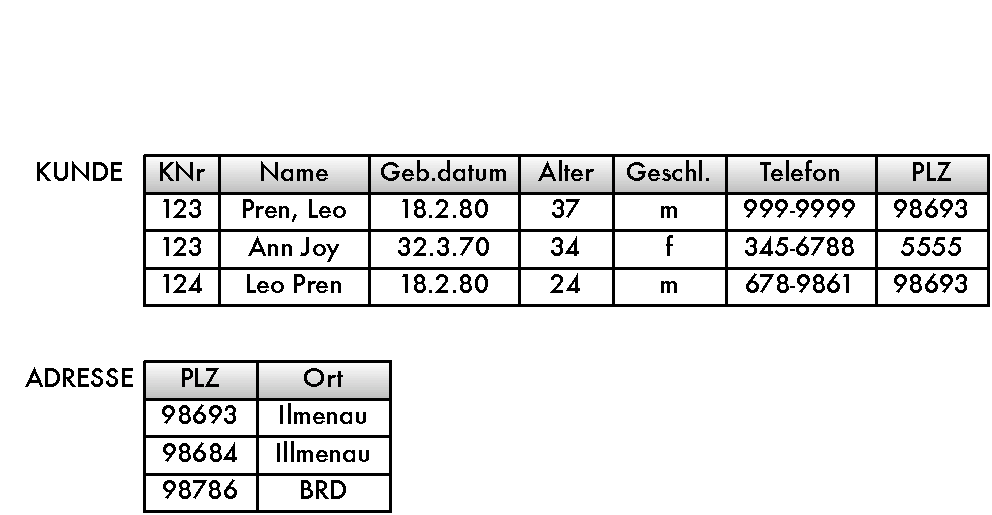
\includegraphics[scale=.6]{fig4/datenfehler-1.pdf}}
    \only<2>{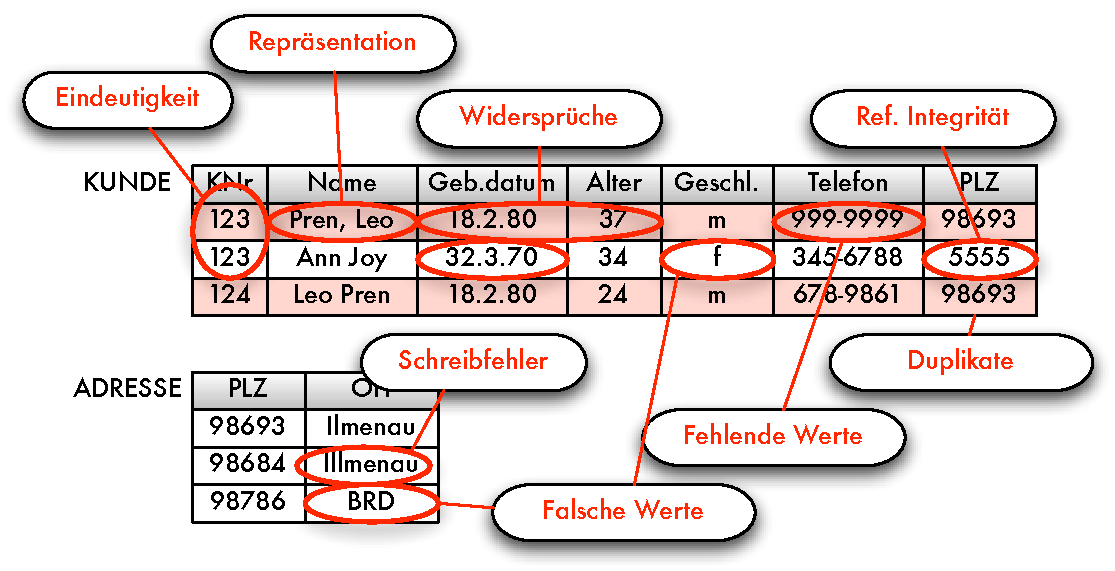
\includegraphics[scale=.6]{fig4/datenfehler-2.pdf}}
    \end{center}
    
    \end{overlayarea}
    \end{frame}
    
    %---------------------------------------------------------------------
    
    \begin{frame}
    \frametitle{Vermeidung von Datenfehlern}
    
    \begin{tabular}{ll}
    \textbf{Vermeidung von}	& \textbf{durch} \\
    \hline
    falschen Datentypen &	Datentypdefinition, \\
    & \op{domain}-Constraints \\
    falschen Werten &	\op{check} \\
    fehlenden Werten &	\op{not null} \\
    ungültigen Referenzen &	\op{foreign key} \\
    Duplikaten &	\op{unique}, \op{primary key} \\
    Inkonsistenzen & Transaktionen \\
    veralteten Daten & Replikation, materialisierte Sichten \\
    \end{tabular}
    \end{frame}
    
    %---------------------------------------------------------------------
    
    \begin{frame}
    \frametitle{Warum dennoch Datenfehler?}
    
    \begin{itemize}
    \item Fehlen von Metadaten, Integritätsbedingungen, \dots
    \item "`fremde"' Daten
    \item Daten aus "`Nicht-DB"'-Quellen
    \item Eingabefehler, Unkenntnis, \dots
    \item Multi-Source-Probleme, Heterogenitäten
    \end{itemize}
    
    \end{frame}
    
    %---------------------------------------------------------------------
    
    \begin{frame}
    \frametitle{Phasen der Datenaufbereitung}
    
    \begin{center}
    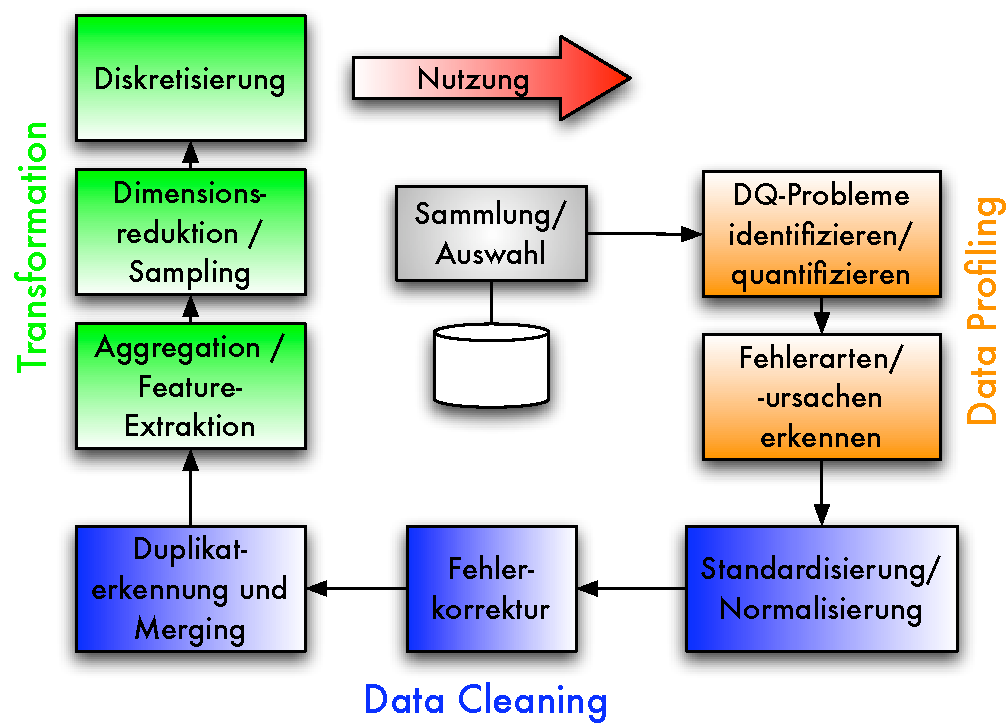
\includegraphics[scale=.5]{fig4/data-preparation.pdf}
    \end{center}
    
    \end{frame}
    
    %---------------------------------------------------------------------
    
    \begin{frame}
    \frametitle{Aufgaben}
    
    \begin{itemize}
    \item Profiling
    \item Homogenisierung und Normalisierung
    \item Behandlung fehlender Daten / Werte
    \item Ausreißererkennung
    \item Record Linkage / Matching, Konfliktbehandlung
    \item Datenaufbereitung: Diskretisierung, Sampling, .... 
    \end{itemize}
    \end{frame}
    
    %---------------------------------------------------------------------
    
    
    \section{Profiling}
    
    
    \frame{
      \frametitle{Überblick}
      \tableofcontents[currentsection,hidesubsections,firstsection=15]
    }
    
    %---------------------------------------------------------------------
    
    \begin{frame}
    \frametitle{Profiling}
    
    \begin{itemize}
    \item Analyse von Inhalt und Struktur einzelner Attribute
    \begin{itemize}
    \item Datentyp, Wertebereich, Verteilung und Varianz, Vorkommen von
      Nullwerten, Eindeutigkeit, Muster (z.B. dd/mm/yyyy) 
    \end{itemize}
    \item Analyse von Abhängigkeiten zwischen Attributen einer Relation
    \begin{itemize}
    \item "`unscharfe"' Schlüssel
    \item Funktionale Abhängigkeiten, potenzielle Primärschlüssel,
      "`unscharfe"' Abhängigkeiten 
    \item Notwendigkeit:
    \begin{itemize}
    \item Keine expliziten Integritätsbedingungen spezifiziert
    \item Jedoch in Daten in den meisten Fällen erfüllt
    \end{itemize}
    \end{itemize}
    \item Analyse von Überlappungen zwischen Attributen verschiedener Relationen
    \begin{itemize}
    \item Redundanzen, Fremdschlüsselbeziehungen
    \end{itemize}
    \end{itemize}
    
    \end{frame}
    
    %---------------------------------------------------------------------
    
    \begin{frame}
    \frametitle{Profiling /2}
    
    \begin{itemize}
    \item Fehlende bzw. falsche Werte
    \begin{itemize}
    \item Ermittelte vs. Erwartete Kardinalität (z.B. Anzahl von Filialen, Geschlecht von Kunden)
    \item Anzahl der Nullwerte, Minimum / Maximum, Varianz
    \end{itemize}
    \item Daten- bzw. Eingabefehler
    \begin{itemize}
    \item Sortierung und manuelle Prüfung
    \item Ähnlichkeitstest
    \end{itemize}
    \item Duplikate
    \begin{itemize}
    \item Tupelanzahl vs. Attributkardinalität
    \end{itemize}
    \end{itemize}
    
    
    \end{frame}
    
    %---------------------------------------------------------------------
    
    
    % \begin{frame}
    % \frametitle{Profiling mit SQL}
    
    % \begin{itemize}
    % \item SQL-Anfragen f�r einfache Profiling-Aufgaben
    % \begin{itemize}
    % \item Schema, Datentypen: Anfragen an Schemakatalog
    % \item Wertebereich
    % \hspace*{-1cm}\begin{sql}
    % \op{select min}(A), \op{max}(A), \op{count}(\op{distinct} A) \\
    % \op{from} Tabelle
    % \end{sql}
    % \item Datenfehler, Defaultwerte
    % \hspace*{-1cm}\begin{sql}
    % \op{select} Ort, \op{count}(*) \op{as} Anz\\
    % \op{from} Kunden \op{group by} Ort \op{order by} Anz
    % \end{sql}
    % \begin{itemize}
    % \item Aufsteigend: Eingabefehler, z.B. Illmenau: 1, Ilmenau: 50
    % \item Absteigend: undokumentierte Default-Werte, z.B. AAA: 80
    % \end{itemize}
    % \end{itemize}
    % \end{itemize}
    % \end{frame}
    
    %---------------------------------------------------------------------
    
    
    \section{Datenbereinigung}
    
    
    \frame{
      \frametitle{Überblick}
      \tableofcontents[currentsection,hidesubsections,firstsection=15]
    }
    
    
    \begin{frame}
    \frametitle{Data Cleaning}
    
    \begin{itemize}
    \item Erkennen \& Beseitigen von Inkonsistenzen, Widersprüchen und
      Fehlern in Daten mit dem Ziel der Qualitätsverbesserung  
    \item Auch Cleansing oder Scrubbing
    \item Bis zu 80\% des Aufwandes in DW-Projekten
    \item Cleaning im DW: Teil des ETL-Prozesses
    \end{itemize}
    
    \end{frame}
    
    %---------------------------------------------------------------------
    
    \begin{frame}
    \frametitle{Normalisierung und Standardisierung}
    
    \begin{itemize}
    \item Datentypkonvertierung: varchar $\rightarrow$ int
    \item Normalisierung: Abbildung in einheitliches Format
    \begin{itemize}
    \item Datum: 03/01/15 $\rightarrow$ 1. März 2015
    \item Währung: \$ $\rightarrow$ \euro
    \item Zeichenketten in Großbuchstaben
    \end{itemize}
    \item Zerlegung in Token: ``Metallica - ...And Justice for All'' $\rightarrow$ ``Metallica'', ``...And Justice for All''
    \item Diskretisierung numerischer Werte (Aufteilung von Wertebereichen in Intervalle, z.B. Altersgruppen)
    \item Domänenspezifische Transformationen
    \begin{itemize}
    \item Codd, Edgar Frank $\rightarrow$ Edgar Frank Codd
    \item Str. $\rightarrow$ Straße
    \item Adressen über Adressdatenbanken
    \item Branchenspezifische Produktbezeichnungen
    \end{itemize}
    \end{itemize}
    
    \end{frame}
    
    %---------------------------------------------------------------------
    
    \begin{frame}
    \frametitle{Normalisierung numerischer Daten}
    
    \begin{itemize}
    \item Skalierung der Werte $v$ eines Attributs $A$ mit $[min_A,max_A]$
      in vorgegebenen Bereich $[min_{new},max_{new}]$, z.B. $[0, 1]$
    % \item notwendig u.a. f�r distanzbasierte Verfahren
    % \item Techniken
    \begin{itemize}
    \item Min-Max-Normalisierung
    $$
    v' = \frac{v - min_A}{max_A - min_A}(max_{new} - min_{new}) +
    min_{new}
    $$
    \item Z-Score-Normalisierung: basierend auf Mittelwert und
      Standardabweichung
    $$
    v' = \frac{v - \mu}{\sigma}
    $$
    \begin{itemize}
    \item speziell wenn $min_A$, $max_A$ nicht bekannt sind oder bei
      dominierenden Ausreißern
    \end{itemize}
    \item Dezimalskalierung: "`Verschieben"' des Dezimalpunktes
    $$
    v' = \frac{v}{10^i}\;\text{mit}\;i\;\text{ist kleinster ganzzahliger
      Wert, sodass}\;max(|v'|) < 1
    $$
    \end{itemize}
    
    \end{itemize}
    
    \end{frame}
    
    %---------------------------------------------------------------------
    
    \begin{frame}
    \frametitle{Fehlende Werte}
    
    \begin{itemize}
    \item Fehlen von Daten auf unterschiedlichen Ebenen
    \begin{itemize}
    \item Instanzebene: Werte, Datensätze, Teilrelationen, ...
    \item Schemaebene: Attribute, ...
    \end{itemize}
    \item Problem speziell auf Instanzebene:
    \begin{itemize}
    \item Behandlung von Nullwerten: Unterscheidung fehlender Wert, Defaultwert oder Dummywert? 
    \item "`Abschneiden"' von Werten
    \end{itemize}
    \item Verzerrungen von Erwartungswerten, Fehler durch Nullwerte
    \end{itemize}
    
    \end{frame}
    
    %---------------------------------------------------------------------
    
    \begin{frame}
    \frametitle{Fehlende Werte: Erkennung}
    
    \begin{itemize}
    \item Einfache Analysen: 
    \begin{itemize}
    \item Anzahl der Nullwerte, Duplikate, Mittelwerte, Häufigkeiten
    \item Vergleich mit Erwartungswerten
    \item Für DW-Daten auch auf verschiedenen Aggregationsebenen
    \end{itemize}
    \item Analyse der "`Ordnung"' der Datensätze
    \begin{itemize}
    \item Keine Verkaufszahlen vom 1.3.-4.3.?
    \item Keine Produkte im Preissegment > 20 \euro?
    \end{itemize}
    \item "`Verstümmelte"' Daten, z.B. durch Abschneiden von Werten
    \begin{itemize}
    \item Einkäufe unter 1 \euro\ nicht berücksichtigt
    \item Einkäufe über 100 \euro\ als 100 \euro\ behandelt
    \end{itemize}
    \item Erkennung
    \begin{itemize}
    \item Hinweise durch Analyse der Datenverteilung
    \item Meist jedoch Domänenwissen notwendig 
    \end{itemize}
    \end{itemize}
    
    \end{frame}
    
    %---------------------------------------------------------------------
    
    
    \begin{frame}
    \frametitle{Fehlende Werte: Behandlung}
    
    \begin{itemize}
    \item "`unbiased estimators"'
    \begin{itemize}
    \item Wertschätzung ohne Änderung der Charakteristika der
      existierenden Daten (Mittelwert, Standardabweichung, \dots) 
    \item Beispiel: 1, 2, 3, \_, 5
    \begin{itemize}
    \item Mittelwert erhalten $\rightarrow$ 2.75
    \item Standardabweichung erhalten $\rightarrow$ 4.659
    \end{itemize}
    \end{itemize}
    \item Ausnutzung von Attributbeziehungen
    \begin{itemize}
    \item Bsp.: Hausgröße $\rightarrow$ Einkommen
    \end{itemize}
    \item Statistik-Techniken
    \begin{itemize}
    \item Lineare Regression: Einkommen = c $\cdot$ Hausgröße
    \item Techniken für nichtlineare Zusammenhänge: Neuronale Netze, \dots
    \end{itemize}
    \end{itemize}
    
    \end{frame}
    
    %---------------------------------------------------------------------
    
    \begin{frame}
    \frametitle{Profiling mit Pandas}
    
    \begin{itemize}
    \item Überblick zu den Daten
    \end{itemize}
    
    \begin{python}
    \prompt{In [10]:} kreise.describe()
    \end{python}
    
    \begin{itemize}
    \item Verteilung der Attributwerte
    \end{itemize}
    
    \begin{python}
    \prompt{In [11]:} kreise.hist(bins=20, figsize=(30,25))
    \end{python}
    
    \begin{itemize}
    \item Plotten der Korrelationen
    \end{itemize}
    
    \end{frame}
    
    %---------------------------------------------------------------------
    
    \begin{frame}
    \frametitle{Ausreißererkennung}
    
    \begin{itemize}
    \item Ausreißer: Wert der nicht in eine erwartete Messreihe passt
    \item Aspekte:
    \begin{itemize}
    \item Erkennung: Verteilung, "`Geometrie"', Zeitreihe
    \item Interpretation: Mess- bzw. Datenfehler oder echtes Ereignis
    \end{itemize}
    \begin{center}
    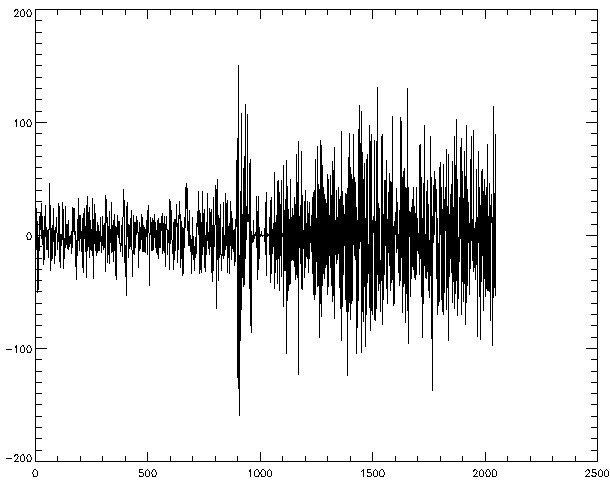
\includegraphics[width=4cm]{fig4/noise2.png}\quad
    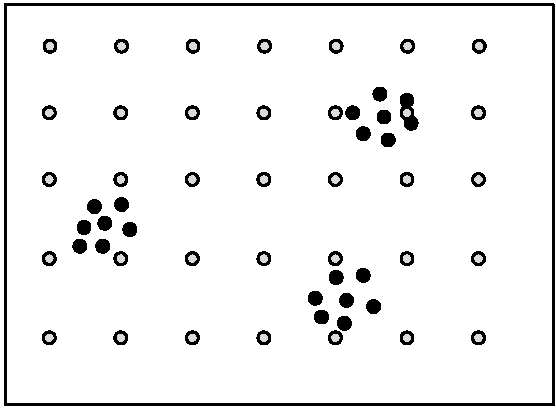
\includegraphics[width=4cm]{fig4/noise1.pdf}
    \end{center}
    \end{itemize}
    
    \end{frame}
    
    %---------------------------------------------------------------------
    
    \begin{frame}
    \frametitle{Ausreißererkennung /2: Erkennung }
    
    \begin{itemize}
    \item Modellbasiert: Ableitung einer Beziehung von Attributen
        \begin{itemize}
        \item lineare Regression
        \item Regeln: WENN Alter $<$ 16 DANN Führerschein IS NULL
        \end{itemize}
    \item Verteilungs- bzw. statistikbasiert: 
        \begin{itemize}
        \item z.B. Verwendung von Boxplots / Box-Whisker-Plots (außerhalb des Whiskers $\rightarrow$ Ausreißer)
        \end{itemize}
    
    \item Geometrisch und distanzbasiert:
    \begin{itemize}
    \item Peeling: "`Schichten"' im Datenraum mit wachsender Tiefe
    \begin{itemize}
    \item äußere Schichten enthalten Ausreißer
    \item Nicht praktikabel für höhere Dimensionsanzahl
    \end{itemize}
    \item Distanzbasiert: Abstand zwischen Datenpunkten (metrische
      Distanzfunktion) 
    \begin{itemize}
    \item Für Anwendungen ohne Standardverteilung
    \item Bei größerer Dimensionsanzahl
    \end{itemize}
    \end{itemize}
    \end{itemize}
    
    
    \end{frame}
    
    %---------------------------------------------------------------------
    
    \begin{frame}
    \frametitle{Distanzbasierte Ausreißer (\emph{DB})}
    
    \begin{itemize}
    \item Objekt $o$ aus Datenmenge $T$ ist Ausreißer $DB(p,D)$, wenn
      mindestens ein Anteil $p$ von $T$ weiter als $D$ von $o$ entfernt
      ist [Knorr Ng 1998] 
    \begin{columns}[c]
    \begin{column}{5cm}
    \begin{itemize}
    \item Ausreißer: "`Objekte, die nicht genug Nachbarn besitzen"'
    \item $p$ als Parameter zur Anpassung, falls Cluster von Ausreißern
    \item Bsp. Standardnormalverteilung: $DB(0.998, 0.13\sigma)$, $d \approx 3$
    \end{itemize}
    \end{column}
    \begin{column}{5cm}
    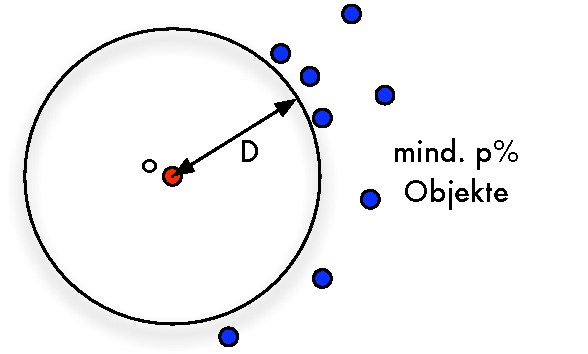
\includegraphics[scale=.6]{fig4/distance-outlier.pdf}
    \end{column}
    \end{columns}
    
    \end{itemize}
    
    
    \end{frame}
    
    
    %---------------------------------------------------------------------
    
    \begin{frame}
    \frametitle{Record Linkage}
    
    \begin{itemize}
    \item Identifikation von semantisch äquivalenten Datensätzen, d.h. die
      das gleiche Realwelt-Objekt repräsentieren
    \item auch: Object Identification, Duplicate Elimination, Merge/Purge
    \begin{itemize}
    \item Merge: Erkennen von Duplikaten
    \item Purge: Auswahl /Berechnung des "`besten"' Vertreters pro Klasse
    \end{itemize}
    \end{itemize}
    
    \begin{center}
    {\small\begin{tabular}{|c|l|l|}
    \hline
    \rowcolor{Gray} KundenNr & Name & Adresse \\
    \hline \hline
    3346 & Just Vorfan & Hafenstraße 12 \\
    3346 & Justin Forfun & Hafenstr. 12 \\
    \hline
    5252 & Lilo Pause & Kuhweg 42 \\
    5268 & Lisa Pause & Kuhweg 42 \\
    \hline
    $\perp$ & Ann Joy & Domplatz 2a \\
    $\perp$ & Anne Scheu & Domplatz 28 \\
    \hline
    \end{tabular}}
    \end{center}
    
    \end{frame}
    
    %---------------------------------------------------------------------
    \begin{frame}
    \frametitle{Record Linkage: Vergleiche}
    
    \begin{itemize}
    \item Typische Vergleichsregeln
    
    \hspace*{-1cm}\begin{sql}
    \op{if} ssn1=ssn2 \op{then} match \\
    \op{else} \op{if} name1=name2 \op{then} \\
    \1  \op{if} firstname1=firstname2 \op{then} \\
    \2    \op{if} adr1=adr2 \op{then} match \\
    \2    \op{else} unmatch \\
    \1  \op{else} \op{if} adr1=adr2 \op{then} match\_household \\
    \op{else} \op{if} adr1=adr2 \op{then} \\
     ...
    \end{sql}
    
    \item Naiver Ansatz: "`Jeder-gegen-jeden"'
    \begin{itemize}
    \item $O(n^2)$ Vergleiche
    \item Maximale Genauigkeit (je nach Regeln)
    \item Viel zu teuer
    \end{itemize}
    \end{itemize}
    
    \end{frame}
    
    %---------------------------------------------------------------------
    
    \begin{frame}
    \frametitle{Record Linkage: Prinzip}
    
    \begin{center}
    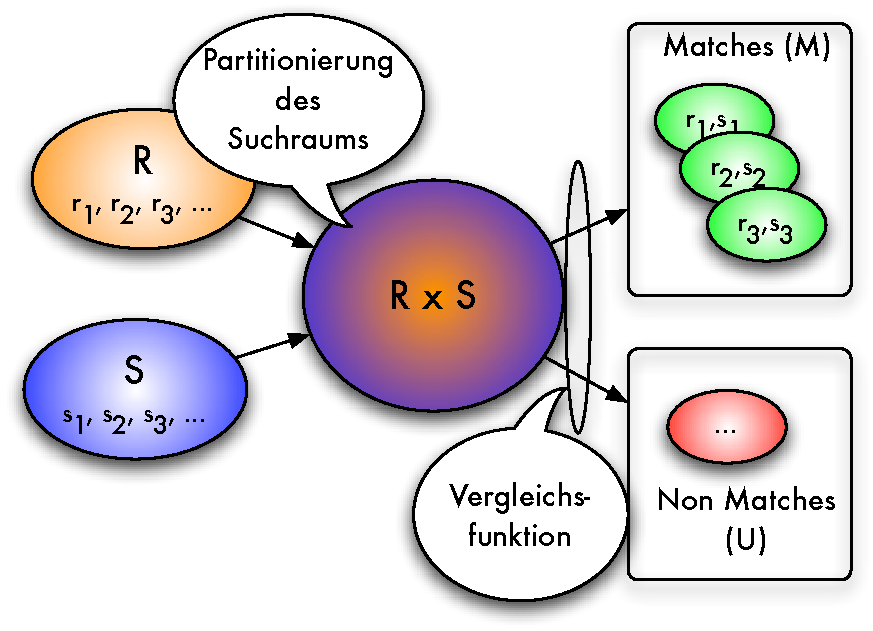
\includegraphics[scale=.6]{fig4/record-linkage.pdf}
    \end{center}
    
    \end{frame}
    
    %---------------------------------------------------------------------
    
    
    \begin{frame}
    \frametitle{Partitionierung}
    
    \begin{itemize}
    \item \hl{Blockung}
    \begin{itemize}
    \item Aufteilung des Suchraums in disjunkte Blöcke
    \item Duplikate nur innerhalb eines Blockes 
    \item Bsp.: PLZ-Partitionierung 01*** bis 99***, Name nach Anfangsbuchstaben
    \end{itemize}
    \item \hl{Sortierte Nachbarschaft} [Hernandez Stolfo 1998]
    \begin{itemize}
    \item Sortiert Tupel, so dass ähnliche Tupel nah beieinander liegen
    \item Vergleiche nur in einer engen Nachbarschaft
    \end{itemize}
    \item \hl{Multi-Pass-Technik}
    \begin{itemize}
    \item Transitive Hülle über verschiedene Sortierungen
    \end{itemize}
    \end{itemize}
    
    \end{frame}
    
    %---------------------------------------------------------------------
    
    
    \begin{frame}
    \frametitle{Sortierte Nachbarschaft}
    
    \begin{itemize}
    \item Sortierung der Daten anhand eines gewählten Schlüssels
    \item Vergleiche in einem gleitenden Fenster
    \end{itemize}
    
    \begin{columns}[c]
    \begin{column}{7.5cm}
    \begin{enumerate}
    \item Berechne einen Schlüssel pro Record
    \begin{itemize}
    \item Bsp: SSN + "`ersten 3 Zeichen von Name"' + ...
    \item Beachtung typischer Fehler: 0-O, Soundex, Nachbartasten, ...
    \end{itemize}
    \item Sortiere nach Schlüssel
    \item Laufe Liste sequenziell ab
    \item Vergleiche innerhalb eines Windows $W$, $|W|=w$
    \end{enumerate}
    \end{column}
    \begin{column}{3.5cm}
    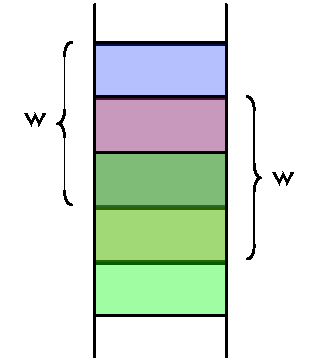
\includegraphics[scale=.6]{fig4/sorted-neighborhood.pdf}
    \end{column}
    \end{columns}
    
    % \begin{itemize}
    % \item Komplexität: % $O(n \cdot \log(n))$ oder $O(n \cdot w)$
    % \begin{itemize}
    % \item Schlüsselerzeugung: $O(n)$, Sortieren: $O(n \cdot \log(n))$;
    %   Vergleichen: $O( (n/w) \cdot (w^2)) = O(n \cdot w)$; 
    % Gesamt: $O(n \cdot \log(n))$ oder $O(n \cdot w)$
    % \end{itemize}
    % \end{itemize}
    
    \end{frame}
    
    %---------------------------------------------------------------------
    
    \begin{frame}
    \frametitle{Sortierte Nachbarschaft: Probleme}
    
    \begin{itemize}
    \item Genauigkeit schlecht
    \begin{itemize}
    \item Sortierkriterium bevorzugt immer Attribute
    \item Sind erste Buchstaben wichtiger für Identität als letzte?
    \item Ist Nachname wichtiger als Hausnummer?
    \end{itemize}
    \item Window vergrößern?
    \begin{itemize}
    \item Keine Hilfe
    \item Dominanz eines Attributes bleibt gleich, aber Laufzeit
      verschlechtert sich schnell 
    \end{itemize}
    \end{itemize}
    
    \end{frame}
    
    %---------------------------------------------------------------------
    
    
    \begin{frame}
    \frametitle{Multi-Pass-Technik}
    
    \begin{itemize}
    \item Sortieren und vergleichen nach mehreren Kriterien
    \item Kleinere Fenster
    \item Bildung der transitiven Hülle der Duplikate bis zu gegebener Länge
    \end{itemize}
    
    \begin{columns}[c]
    \begin{column}{6cm}
    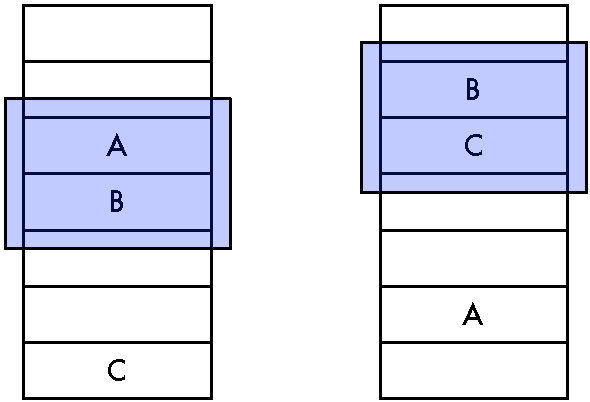
\includegraphics[scale=.6]{fig4/multi-pass.pdf}
    \end{column}
    \begin{column}{5cm}
    \begin{itemize}
    \item 1. Lauf: "`A matches B"'
    \item 2. Lauf: "`B matches C"'
    \item Transitivität: "`A matches C"'
    \end{itemize}
    \end{column}
    \end{columns}
    
    \end{frame}
    
    %---------------------------------------------------------------------
    
    
    \begin{frame}
    \frametitle{Vergleichsfunktionen}
    
    \begin{itemize}
    \item Vergleichsfunktionen für Felder (String $A$ und $B$), u.a.:
    \begin{itemize}
    \item \hl{Editierdistanz}: Anzahl der Editieroperationen (Einfügen,
      Löschen, Ändern) für Änderung von $A$ in $B$ 
    \item \hl{q-Grams}: Vergleich der Mengen aller Teilstrings von $A$ und $B$
      der Länge $q$ 
    \item \hl{Jaro-Distanz}: Berücksichtigung von gemeinsamen Zeichen
      (innerhalb der halben Stringlänge) und transponierten Zeichen (an
      anderer Position) 
    \item Jaccard, TFIDF, Soundex, ...
    \end{itemize}
    \end{itemize}
    
    \end{frame}
    %---------------------------------------------------------------------
    
    \begin{frame}
    \frametitle{Vergleichsfunktionen: Editierdistanz}
    
    \begin{itemize}
    \item \hl{Editierdistanz} (Levensthein-Distanz):
    \begin{itemize}
    \item Anzahl der Editieroperationen (Einfügen, Löschen, Ändern) für
      Änderung von $A$ in $B$  
    \item Beispiel:
    \hspace*{-1cm}\begin{sql}
    edit\_distance("Qualität", "Quantität") = 2 \\
    \1 $\Rightarrow$ update(3,'n') \\
    \1 $\Rightarrow$ insert(4,'t')
    \end{sql}
    \item Anwendung:
    \hspace*{-1cm}\begin{sql}
    \op{select} P1.Name, P2.Name \\
    \op{from} Produkt P1, Produkt P2 \\
    \op{where} edit\_distance(P1.Name, P2.Name) $<=$ 2
    \end{sql}
    \end{itemize}
    \end{itemize}
    
    \end{frame}
    
    %---------------------------------------------------------------------
    
    \begin{frame}
    \frametitle{Vergleichsfunktionen: q-Grams}
    
    \begin{itemize}
    \item \hl{q-Grams}: Menge aller Substrings der Länge $q$\\
    Qualität := \{ \_\_Q, \_Qu, Qua, ual, ali, lit, itä, tät, ät\_, t\_\_ \}
    \item Beobachtung: Strings mit kleiner Editierdistanz haben viele
      gemeinsame q-Grams, d.h. für Editierdistanz = $k$ mind.
    $$\max(|A|, |B|)-1-(k-1) \cdot q$$
     gemeinsame q-Grams
    
    \item \hl{Positionale q-Grams}: Ergänzung um Position im String \\
    Qualität := \{ (-1, \_\_Q), (0, \_Qu), (1, Qua), ... \}
    \begin{itemize}
    \item Filterung für effizienten Vergleich:
    \begin{itemize}
    \item COUNT: Anzahl der gemeinsamen q-Grams
    \item POSITION: Positionsunterschied zwischen korrespondierenden
      q-Grams $\leq$ k 
    \item LENGTH: Differenz der Stringlängen $\leq$ k
    \end{itemize}
    \end{itemize}
    \end{itemize}
    
    \end{frame}
    
    %---------------------------------------------------------------------
    
    \begin{frame}
    \frametitle{Domänenspezifische Vergleichsfunktionen}
    
    \begin{itemize}
    \item Vergleiche in Feldern mit spezieller Bedeutung (Namen, Codes,
      Adressen)
    \begin{itemize}
    \item Soundex: phonetische Kodierung, speziell für ähnlich klingende
      Namen ("Hilbert" = "Heilbpr") 
    \item Ausnutzung von Codes (TXL = Berlin-Tegel)
    \item Namenskonventionen
    \begin{itemize}
    \item Hawking, Stephen = Stephen Hawking
    \item Hauptstr. = Hauptstraße
    \end{itemize}
    \end{itemize}
    \end{itemize}
    
    \end{frame}
    
    %---------------------------------------------------------------------
    %
    %\begin{frame}
    %\frametitle{Vergleich von Records}
    %
    %\begin{itemize}
    %\item Basierend auf �hnlichkeit der Felder
    %\item Problem:
    %\begin{itemize}
    %\item Feldanzahl und Art k�nnen sich unterscheiden
    %\item Auswahl relevanter Felder
    %\item Wichtung der Felder
    %\begin{itemize}
    %\item 8 Pkt. f�r �bereinstimmung Nachname
    %\item 6 Pkt. f�r f�r �bereinstimmung Vorname
    %\item 4 Pkt. f�r f�r �bereinstimmung Geburtstag
    %\item 1 Pkt. f�r f�r �bereinstimmung Geschlecht
    %\item Gesamt �ber 11 Pkt. $\rightarrow$ Treffer
    %\end{itemize}
    %\end{itemize}
    %\item Ans�tze
    %\begin{itemize}
    %\item Probabilistische Verfahren 
    %\item Nicht-Probabilistische Verfahren
    %\end{itemize}
    %\end{itemize}
    %
    %\end{frame}
    %
    %%---------------------------------------------------------------------
    %
    %\begin{frame}
    %\frametitle{Probabilistische Verfahren}
    %
    %\begin{center}
    %\includegraphics[scale=.6]{fig3/prob-linkage.pdf}
    %\end{center}
    %
    %\end{frame}
    %
    %%---------------------------------------------------------------------
    %
    %\begin{frame}
    %\frametitle{Probabilistische Verfahren /2}
    %
    %\begin{itemize}
    %\item Vergleichsvektor enth�lt "`Features"' $\gamma(R.A_i,S.A_i)$
    %\begin{itemize}
    %\item z.B. "`Nachnamen sind gleich"'
    %\end{itemize}
    %$$
    %\gamma = (\gamma^1(t_R.A_1,t_S.A_1), \gamma^2(t_R.A_2,t_S.A_2), \dots,
    %\gamma^k(t_R.A_k,t_S.A_k))$$
    % 
    %\item Wahrscheinlichkeiten
    %\begin{itemize}
    %\item $m(\gamma) = P(\gamma | (t_R, t_S) \in M)$ f�r Match
    %\item $u(\gamma) = P(\gamma | (t_R, t_S) \in U)$ f�r Non-Match
    %\item Ableitung von $m(\gamma)$ und $u(\gamma)$ z.B. durch
    %  Voruntersuchung (z.B. EM-Algorithmus (Expectation-Maximization-Algorithmus))
    %\end{itemize}
    %\item Ablauf
    %\begin{enumerate}
    %\item Bestimmung der Einzelgewichte f�r Attribute
    %\item Berechnung des Gesamt-Scores
    %\item Entscheidung �ber Match (M) bzw. Non-Match (U)
    %\end{enumerate}
    %\end{itemize}
    %
    %\end{frame}
    %
    %%---------------------------------------------------------------------
    %
    %\begin{frame}
    %\frametitle{Nicht-Probabilistische Verfahren (Deterministische Verfahren)}
    %
    %\begin{itemize}
    %\item Wissensbasierte Verfahren
    %\begin{itemize}
    %\item Funktionale Abh�ngigkeiten auf Instanzebene
    %\item Matching-Regeln
    %\end{itemize}
    %\item Data-Mining-Verfahren
    %\begin{itemize}
    %\item Clustering
    %\item Entscheidungsbaumverfahren
    %\end{itemize}
    %\item Distanzbasierte Verfahren
    %\end{itemize}
    %
    %\end{frame}
    %
    %%---------------------------------------------------------------------
    %
    %\begin{frame}
    %\frametitle{Regelbasiertes Matching}
    %
    %\begin{itemize}
    %\item IntelliClean [Lee et al. 2000]
    %\item Nutzung von Dom�nenwissen durch deklarative Regeln
    %\hspace*{-1cm}\begin{sql}
    %\op{if} A.Name = B.Name \\
    %\op{and} field\_similarity (A.Adresse, B.Adresse) \\
    %\op{then} \dots 
    %\end{sql}
    %\item Regeltypen
    %\begin{itemize}
    %\item Duplicate identification rules: Bedingungen f�r �bereinstimmung
    %  mit Sicherheitsfaktor 
    %\item Merge/purge rules: Aktionen zum Verschmelzen
    %\item Update rules: Manipulation von Feldern (z.B. bei leeren Feldern)
    %\item Alert rules: Benachrichtigung bei notwendigem Review
    %\end{itemize}
    %\item Regelauswertung durch Inferenz-Engine
    %\end{itemize}
    %
    %\end{frame}
    %---------------------------------------------------------------------
    
    \begin{frame}
    \frametitle{Datenkonflikte}
    
    \begin{itemize}
    \item Datenkonflikt: Zwei Duplikate haben unterschiedliche
      Attributwerte für semantisch gleiches Attribut
    \begin{itemize}
    \item im Gegensatz zu Konflikten mit Integritätsbedingungen
    \item Bsp.: Amazon\\
    \begin{tabular}{|l|l|l|c|}
    \hline
    0766607194 & H. Melville & & 3.99 \\
    \hline
    0766607194 & Herman Melville &  Moby Dick & 5.99 \\
    \hline
    \end{tabular}
    
    \end{itemize}
    
    \item Datenkonflikte entstehen 
    \begin{itemize}
    \item innerhalb eines Informationssystems (intra-source) und
    \item bei der Integration mehrerer Informationssysteme (inter-source)
    \end{itemize}
    \item Voraussetzung: Duplikat, d.h. Identität schon festgestellt
    \item erfordert: Konfliktauflösung (Purging, Reconciliation)
    \end{itemize}
    
    \end{frame}
    
    %---------------------------------------------------------------------
    
    
    \begin{frame}
    \frametitle{Datenkonflikte: Entstehung}
    
    \begin{itemize}
    \item Mangels Integritätsbedingungen oder Konsistenz-Checks
    \item Bei redundanten Schemata
    \item Bei Entstehung von Duplikaten
    \item Nicht korrekte Einträge
    \begin{itemize}
    \item Tippfehler, Übertragungsfehler
    \item Falsche Rechenergebnisse
    \end{itemize}
    \item obsolete Einträge
    \begin{itemize}
    \item div. Aktualisierungszeitpunkte
    \begin{itemize}
    \item ausreichende Aktualität einer Quelle
    \item verzögerte Aktualisierung
    \end{itemize}
    \item vergessene Aktualisierung
    \end{itemize}
    \end{itemize}
    
    
    \end{frame}
    
    
    %---------------------------------------------------------------------
    
    \begin{frame}
    \frametitle{Datenkonflikte: Behebung}
    
    \begin{itemize}
    \item Referenztabellen für exakte Wertabbildung
    \begin{itemize}
    \item Z.B. Städte, Länder, Produktnamen, Codes...
    \end{itemize}
    \item Ähnlichkeitsmaße
    \begin{itemize}
    \item bei Tippfehlern, Sprachvarianten (Meier, Mayer,...)
    \end{itemize}
    \item Standardisieren und Transformieren
    \item Nutzung von Hintergrundwissen (Metadaten)
    \begin{itemize}
    \item bzgl. Konventionen (landestypische Schreibweisen)
    \item Ontologien, Thesauri, Wörterbücher zur Behandlung von Homonymen,
      Synonymen, \dots
    \end{itemize}
    \item Bei der Integration
    \begin{itemize}
    \item Präferenzordnung über Datenquellen nach Aktualität, Trust
      (Vertrauen) usw. 
    \item Konfliktlösungsfunktionen
    \end{itemize}
    \end{itemize}
    
    \end{frame}
    
    
    %---------------------------------------------------------------------
    
    \begin{frame}
    \frametitle{Record Linkage mit Python Record Linkage Toolkit}
    
    \begin{itemize}
    \item Python-Framework für Record Linkage-Aufgaben
    \item Komponenten
    \begin{itemize}
    \item Indexer: Komponente zur Gruppierung von Kandidaten, z.B. Blocking und Sortierte Nachbarschaft
    \item Vergleichs- und Ähnlichkeitsfunktionen
    \item Klassifikatoren für Einteilung in Matches / Non-Matches
    \item Datensätze
    \end{itemize}
    \item nutzbar mit Pandas 
    \end{itemize}
    
    \end{frame}
    
    %---------------------------------------------------------------------
    
    \begin{frame}[shrink]
    \frametitle{Python Record Linkage Toolkit}
    
    \begin{python}
    \pycomment{Daten laden} \\
    from recordlinkage.datasets import load\_febrl1 \\
    data = load\_febrl1() \\
    \pycomment{Blocking als Indexer nutzen} \\
    indexer = recordlinkage.Index() \\
    indexer.block('given\_name') \\
    \pycomment{Kandidaten für Vergleiche} \\
    candidates = indexer.index(data) \\
    \\
    \pycomment{Vergleichsfunktion} \\
    cmp = recordlinkage.Compare() \\
    cmp.exact('given\_name', 'given\_name', label='given\_name') \\
    cmp.string('surname', 'surname', method='jarowinkler', \\
    \1 threshold=0.85, label='surname') \\
    ...\\
    features = cmp.compute(candidates, data) 
    \end{python}
    
    \end{frame}
    
    %---------------------------------------------------------------------
    \begin{frame}
    \frametitle{Python Record Linkage Toolkit: Matching}
    
    \begin{itemize}
    \item DataFrame \texttt{features} enthält alle Record-Paare und die Features
    \item Summieren der Werte pro Zeile (\texttt{axis=1})
    \end{itemize}
    \begin{python}
    features.sum(axis=1).value\_counts().\textbackslash \\
    \1 sort\_index(ascending=False)
    \end{python}
    
    \begin{itemize}
    \item Auswahl über Schwellwert
    \end{itemize}
    
    \begin{python}
    matches = features[features.sum(axis=1) > 3]
    \end{python}
    
    \end{frame}
    %---------------------------------------------------------------------
    
    \section{Datenreduktion}
    
    \begin{frame}
    \frametitle{Datenreduktion}
    
    
    \begin{itemize}
    \item \hl{Ziel:} Reduzierung der Daten
    \begin{itemize}
    \item kleinere Datenmenge $\leadsto$ schnellere Verarbeitung: \hl{Sampling}
    \item Eliminierung irrelevanter Daten: \hl{Dimensionsreduktion} z.B. durch Hauptkomponentenanalyse (PCA)
    \item Erhöhung des Abstrationslevels: \hl{Aggregation}, \hl{Diskretisierung}
    \end{itemize}
    \item Erhaltung der Konsistenz der Daten
    \end{itemize}
    \end{frame}
    
    %---------------------------------------------------------------------
    
    \begin{frame}
    \frametitle{Sampling}
    
    \begin{itemize}
    \item Idee: kleine, zufällig gewählte, uniforme Stichprobe $S$ stellt gute
      Repräsentation der Daten (Grundgesamtheit) dar
    \begin{itemize}
    \item Datenreduktion
    \item Erzeugung eines Testdatensatzes zur Validierung
    \item approximiertes Anfrageergebnis: Ausführung einer modifizierten
      Anfrage auf $S$
    \end{itemize}
    \item Beispiel:
    
    {\small
    \begin{tabular}{ccccccccccccccc}
    3 & \fbox{4} & 7 & \fbox{8} & 6 & 1 & \fbox{2} & 5 & \fbox{9} & 6 & 2
    & \fbox{7} & 4 & 6 & \fbox{1}
    \end{tabular}}
    \vspace*{.5em}
    
    \hspace*{-.5cm}\begin{algo}
    \op{select} \emph{aggr} \op{from} Data \op{where} item > 5
    \end{algo}
    \begin{itemize}
    \item \emph{aggr} = \texttt{avg} $\leadsto$ 8 (exakt: 7)
    \item \emph{aggr} = \texttt{count} für $\frac{3}{6}$ $\leadsto$ 7.5 (exakt: 7)
    \end{itemize}
    \end{itemize}
    \end{frame}
    
    %---------------------------------------------------------------------
    
    \begin{frame}
    \frametitle{Sampling: Verfahren}
    
    \begin{itemize}
    \item \hl{einfaches randomisiertes Sampling:} jedes Element der Grundgesamtheit ist mit der gleichen Wahrscheinlichkeit in der Stichprobe enthalten
    \item \hl{stratifiziertes ("`geschichtetes") Sampling:} 
    \begin{itemize}
    \item Aufteilung der Grundgesamtheit in Gruppen (Strata, Schichten)
    \item Festlegung der Stichprobengröße pro Schicht
    \item Sampling pro Schicht
    \item \hl{erfordert Vorabkenntnis der Schichtungsmerkmale}, z.B. Bevölkerungsgruppen bei Wahlen
    \end{itemize}
    \item \hl{Cluster Sampling:} Clustering der Daten, zufallsbasierte Auswahl der Cluster, alle Elemente der gewählten Cluster bilden Stichprobe $\leadsto$ Reduzierung des Erhebungsaufwandes (Befragung etc.)
    \end{itemize}
    \end{frame}
    
    %---------------------------------------------------------------------
    
    \begin{frame}
    \frametitle{Reservoir-Sampling}
    
    [Vitter 85]
    \begin{itemize}
    \item Ziel: Verwaltung einer zufälligen Stichprobe konstanter Größe
      für Grundgesamtheit \textbf{unbekannter Größe} (z.B. Datenstrom)
    \end{itemize}
    
    \begin{center}
    \includegraphics[scale=.7]{fig4/reservoir-sampling.pdf}
    \end{center}
    
    \end{frame}
    
    %---------------------------------------------------------------------
    
    \begin{frame}
    \frametitle{Reservoir-Sampling /2}
    
    \begin{itemize}
    \item Prinzip
    \begin{itemize}
    \item Übernahme der ersten $k$ Elemente des Stroms in das Reservoir
      $S$
    \item Ankunft des $i$-ten Elementes
    \begin{itemize}
    \item zum Reservoir $S$ hinzufügen mit Wahrscheinlichkeit
      $\frac{k}{i}$
    \item falls hinzugefügt: zufällig ausgewähltes Element aus $S$ löschen
    \item Test nicht für jedes Element, sondern Anzahl der zu
      überspringenden Elemente im voraus bestimmen
    \end{itemize}
    \end{itemize}
    \end{itemize}
    
    \end{frame}
    
    %---------------------------------------------------------------------
    
    \begin{frame}
    \frametitle{Sampling in Pandas}
    
    \begin{itemize}
    \item Einfaches Sampling eines DataFrames
    \end{itemize}
    \begin{python}
    df.sample(n=10)
    \end{python}
    
    \begin{itemize}
    \item Sampling mit reproduzierbaren Ergebnissen
    \end{itemize}
    \begin{python}
    df.sample(n=10, random\_state=42)
    \end{python}
    
    \begin{itemize}
    \item Sampling mit prozentualer Größe
    \end{itemize}
    
    \begin{python}
    df.sample(frac=0.25, random\_state=42)
    \end{python}
    
    \end{frame}
    
    %---------------------------------------------------------------------
    
    \begin{frame}
    \frametitle{Sampling in Pandas /2}
    
    \begin{itemize}
    \item Aufteilung in Trainings- und Testdaten muss überlappungsfrei sein
    \end{itemize}
    
    \begin{python}
    from sklearn.model\_selection import train\_test\_split \\
    train\_data, test\_data = train\_test\_split(df, \\
    \1 test\_size=0.2, random\_state=42)
    \end{python}
    \end{frame}
    %---------------------------------------------------------------------
    
    \begin{frame}
    \frametitle{Zusammenfassung}
    
    \begin{itemize}
    \item Wiederholung: Statistik und Daten
    \item Daten
    \begin{itemize}
    \item Arten \& Eigenschaften
    \item Datenqualität
    \end{itemize}
    \item Datenbereinigung
    \begin{itemize}
    \item als Teil des Data-Science-Prozesses
    \item wichtige Teilaufgaben: Profiling, fehlende Werte, Ausreißer,
      Record Linkage
    \end{itemize}
    \item Literatur: 
    \begin{itemize}
    \item Ester, Sander: "`Knowledge Discovery in Databases"',
      Springer-Verlag, 2000
    \item Fahrmeir, Künstler, Pigeot, Tutz: "`Statistik -- Der Weg zur
      Datenanalyse"', Springer-Verlag  
    \item Batini, Scannapieco: "`Data Quality: Concepts, Methodologies and
      Techniques"', Springer-Verlag
    \end{itemize}
    \end{itemize}
    
    \end{frame}
    

%%%%%%%%%%%%%%%%%%%%%%%%%%%%%%%%%%%%%%%%%%%%%%%%%%%%%%%%%%%%%%%%%%%%%%


\part{Datenvisualisierung}

\frame[plain,c]{\partpage}

\frame{
  \frametitle{Überblick}
  \tableofcontents[pausesections,hidesubsections,firstsection=21]
}

%\include{graphmining}

%%%%%%%%%%%%%%%%%%%%%%%%%%%%%%%%%%%%%%%%%%%%%%%%%%%%%%%%%%%%%%%%%%%%%%

\part{Data Warehousing und OLAP}

\frame[plain,c]{\partpage}

\frame{
  \frametitle{Überblick}
  \tableofcontents[pausesections,hidesubsections,firstsection=27]
}

%\include{spatiotemporal}

%%%%%%%%%%%%%%%%%%%%%%%%%%%%%%%%%%%%%%%%%%%%%%%%%%%%%%%%%%%%%%%%%%%%%%

\part{Ausgewählte Analyseverfahren: Regression, Klassifikation, Clustering}

\frame[plain,c]{\partpage}

\frame{
  \frametitle{Überblick}
  \tableofcontents[pausesections,hidesubsections,firstsection=33]
}

%\section{Motivation \& Grundlagen}

\begin{frame}
    \frametitle{Motivation}

    \begin{itemize}
        \item bisher: strukturierte Daten in Form von Zahlenwerten in Tabellen oder Datensätzen
        \item aber: 80\% aller Geschäftsdaten liegen als unstrukturierte oder semi-strukturierte Daten ohne bzw. ohne festes Schema vor
    \end{itemize}   

    \vspace*{1cm}
    {\small
    \begin{notebox}
    Text mining, text data mining (TDM) or text analytics is the process of deriving high-quality information from text. It involves "the discovery by computer of new, previously unknown information, by automatically extracting information from different written resources."\\
    \xspace [Source: Wikipedia]
    \end{notebox}
    }

\end{frame}

%----------------------------------------------------

\begin{frame}[c]
    \frametitle{Motivation: Anwendungsgebiete}

    \begin{center}
    \includegraphics[width=\textwidth]{fig8/motivation-1.pdf}
    \end{center}

\small{Thanks to Michael Gertz: Text Analytics WS 2020/21, Uni Heidelberg}
\end{frame}

%----------------------------------------------------

\begin{frame}[c]
    \frametitle{Motivation: Anwendungsgebiete /2}

    \centering\includegraphics[width=\textwidth]{fig8/motivation-2.pdf}
\end{frame}

%----------------------------------------------------

\begin{frame}[c]
    \frametitle{Motivation: Anwendungsgebiete /3}

    \centering\includegraphics[width=\textwidth]{fig8/motivation-3.pdf}
\end{frame}

%----------------------------------------------------

\begin{frame}[c]
    \frametitle{Motivation: Anwendungsgebiete /4}

    \centering\includegraphics[width=\textwidth]{fig8/motivation-4.pdf}
\end{frame}

%----------------------------------------------------

\begin{frame}[c]
    \frametitle{Motivation: Anwendungsgebiete -- NLP}

    \centering\includegraphics[width=\textwidth]{fig8/motivation-5.pdf}
\end{frame}

%----------------------------------------------------

\begin{frame}
    \frametitle{Textanalyse: Grundlagen}

    für die meisten der genannten Anwendungsfälle sind geeignete Textanalyse-Pipelines und -Komponenten essentiell:

    \begin{itemize}
    \item Textvorverarbeitung (Tokenisierung, Normalisierung, \dots)
    \item Textrepräsentation (Vektorraum-Modell, Worteinbettung, \dots)
    \item Textähnlichkeitsmetriken
    \item skalierbare Architekturen für effiziente Verarbeitung großer Datenmengen
    \end{itemize}

    gilt auch für Suchmaschinen, Chatbots, Sprachmodelle, \dots
    %1-24
\end{frame}

%----------------------------------------------------

\begin{frame}
    \frametitle{Textanalyse: Herausforderungen}

    \begin{itemize}
        \item natürliche Sprache ist \hl{symbolbasiert} und \hl{diskret}, mit Grundelementen (Zeichen), aus denen Wörter gebildet werden, die Objekte, Konzepte, Aktionen, Ereignisse etc. bezeichnen
        \item Wörter sind \hl{eindeutige} Symbole, d.h. es besteht keine inhärente Beziehung zwischen den Wörtern
        \item Sprache ist \hl{kompositional}: Buchstaben bilden Wörter, Wörter bilden Phrasen und Sätze
        $\leadsto$ Bedeutung einer Phrase ist mehr als die Bedeutung einzelner Wörter
    \end{itemize}
   

\end{frame}
%----------------------------------------------------
\begin{frame}
    \frametitle{Textanalyse: Herausforderungen /2}

    \begin{columns}[c]
        \begin{column}{4cm}
    \includegraphics[width=4cm]{fig8/ntv.png}
        \end{column}
        \begin{column}{4cm}
    \includegraphics[width=3.5cm]{fig8/siri.pdf}
        \end{column}
    \end{columns}

\end{frame}
%----------------------------------------------------

\section{Vorverarbeitung von Textdokumenten}

%----------------------------------------------------

\begin{frame}[c]
    \frametitle{Textvorverarbeitung: Überblick}

\centering\includegraphics[width=\textwidth]{fig8/text-overview.pdf}

\end{frame}

%----------------------------------------------------

\begin{frame}[shrink=10]
    \frametitle{Textdaten}

    \hl{Aufgabe:} Konvertierung von Rohtext in Zeichenfolge
    $\leadsto$ einfach, wenn Dokumente bereits in reinen Textformaten vorliegen

    \textbf{Binärformate:}
    \begin{itemize}
    \item Portable Document Format (PDF)
    \item Microsoft Office format (.doc[x], .ppt[x], .xls[x])
    \item diverse Werkzeuge und Bibliotheken für Konvertierung, z.B. pdf2text, docx (Python), \dots 
    \end{itemize}
    \textbf{Web and Semi-strukturierte Daten:}
    \begin{itemize}
    \item HTML, XML, JSON
    \item umfasst Metadaten zu Stil und Struktur (Entfernen oder Aufbewahren?)
     \end{itemize}
    \textbf{Zeichensatzkodierung:} Unicode, UTF-8, UTF-16, ASMO 708, GBK, \dots
    
\end{frame}


%----------------------------------------------------

\begin{frame}
    \frametitle{Textvorverarbeitung: Schritte}

    \centering\includegraphics[width=\textwidth]{fig8/text-preprocessing.pdf}

% Abbildung ähnlich 2-24
\end{frame}

%----------------------------------------------------

\begin{frame}
    \frametitle{Tokenisierung / Segmentierung}
    
    \hl{Ziel}: Zerlegung von Sätzen und Wörtern in Elemente (Segmente)

    Unterscheidung nach Granularität und Typ:
    \begin{itemize}
    \item Word Tokenizer
    \begin{itemize}
        \item TreebankWordTokenizer -- unter Verwendung von regulären Ausdrücken, orientiert sich an der Penn Treebank
        \item WordPunctTokenizer -- Trennung eines Textes in alphabetische und nicht-alphabetische Zeichen, ebenfalls unter Verwendung eines regulären Ausdrucks
        \item WhitespaceTokenizer -- Trennung eines Textes am Leerzeichen
    \end{itemize}
    \item Sentence Detection -- (intelligente) Satzerkennung (Stichwort: Interpunktion)
    \end{itemize}
\end{frame}
    
%---------------------------------------------------------------------
    
\begin{frame}[fragile]
    \frametitle{Segmentierung: Treebank Word Tokenizer}
    
    \begin{minted}{python}
    import nltk
    # nur beim ersten Verwenden von nltk -
    # laden der trainierten classifier und dictionaries: 
    # nltk.download('all') 
    from nltk.tokenize import word_tokenize
    text="I can't put my hat back on."
    print(word_tokenize(text))
    \end{minted}

    \texttt{$[$'I', 'ca', "n't", 'put', 'my', 'hat', 'back', 'on', '.'$]$}
\end{frame}
    
%---------------------------------------------------------------------
    
\begin{frame}[fragile]
    \frametitle{Segmentierung: Word Punct Tokenizer}
    
    \begin{minted}{python}
    from nltk.tokenize import WordPunctTokenizer 
    s = 'I can't put my hat back on.' 
    WordPunctTokenizer().tokenize(s)
    \end{minted}

    \texttt{$[$'I', 'can', \dq ' \dq, 't', 'put', 'my', 'hat', 'back', 'on', '.'$]$}
\end{frame}
    
 %---------------------------------------------------------------------
    
\begin{frame}[fragile]
    \frametitle{Segmentierung: Whitespace Tokenizer}
   
   \begin{minted}{python}
    from nltk.tokenize import WhitespaceTokenizer
    s = 'I can't put my hat back on.'
    WhitespaceTokenizer().tokenize(s)
    \end{minted}

    \texttt{$[$'I', "can't", 'put', 'my', 'hat', 'back', 'on.'$]$}
\end{frame}
 
%---------------------------------------------------------------------
    
\begin{frame}[fragile]
    \frametitle{Segmentierung: Sentence Detection}
    
    \begin{minted}{python}
    from nltk.tokenize import sent_tokenize
    text = 'I can't put  my hat back on. Mr. X told me so.'
    print(sent_tokenize(text))
    \end{minted}

    \texttt{$[$'I can't put  my hat back on.', 'Mr. X told me so.'$]$}
\end{frame}
    
%----------------------------------------------------

\begin{frame}
    \frametitle{Stemming / Lemmatisierung}
    \hl{Ziel:} unterschiedlich flektierte Wortformen sollen als gleiches Wort (Lexem) erkannt werden
    
    \textbf{Lemmatisierung}
    \begin{itemize}
    \item Ziel: Ermittle das Lemma (Grundform, Zitierform)
    \item Vollformenlexikon
    \item linguistische Analyse der morphologischen Wortuntereinheiten + Lookup 
    \end{itemize}
    Beispiel: 
    fliegt, flog, geflogen etc. $\rightarrow$ fliegen
\end{frame}
    
%---------------------------------------------------------------------
    
\begin{frame}[fragile]
    \frametitle{Lemmatisierung}


    \begin{minted}{python}
    from nltk.stem import WordNetLemmatizer 
    lemmatizer = WordNetLemmatizer()
    print(lemmatizer.lemmatize("corpora"))
    print(lemmatizer.lemmatize("better", pos ='a'))
    \end{minted}

    Deutsch:
    \begin{minted}{python}
    from HanTa import HanoverTagger as ht
    hannover = ht.HanoverTagger('morphmodel_ger.pgz')
    print(hannover.analyze('geflogen'))
    \end{minted}
\end{frame}
    
%---------------------------------------------------------------------
    
\begin{frame}
    \frametitle{Stemming / Lemmatisierung}

    \textbf{Stemming}
    \begin{itemize}
    \item Ziel: Zurückführung von Wörtern auf (künstlichen) Wortstamm
    \item regel-basierter/heuristischer Ansatz
    \item simple Transformationsregeln
    \end{itemize}

    Beispiele: \\
    Museen $\rightarrow$ Muse\\
    essen $\rightarrow$ ess
    
\end{frame}
    
%---------------------------------------------------------------------
    
\begin{frame}[fragile]
    \frametitle{Stemming}

    \begin{minted}{python}
    from nltk.stem.snowball import SnowballStemmer
    snowball = SnowballStemmer("english")
    print ('Snowball: ' + snowball.stem('museum'))
    \end{minted}

    Deutsch:
    \begin{minted}{python}
    from nltk.stem.snowball import SnowballStemmer
    snowball = SnowballStemmer("german")
    print ('Snowball: ' + snowball.stem('Museen'))
    \end{minted}
    \end{frame}
    
    %---------------------------------------------------------------------
    
    \begin{frame}
    \frametitle{Weiteres}
    Weitere Normalisierung:

    \begin{itemize}
    \item Groß- und Kleinschreibung
    \item Schreibfehler korrigieren
    \item Stoppwörter entfernen
    \end{itemize}
\end{frame}
     
%----------------------------------------------------
\begin{frame}
    \frametitle{Stoppwort-Eliminierung}

    \hl{Ziel:} Entfernen nicht-relevanter/semantikarmer Wörter

    \centering\includegraphics[width=\textwidth]{fig8/stopwords_example1}

\end{frame}
     
%----------------------------------------------------
\begin{frame}
    \frametitle{Stoppwort-Eliminierung}

    \hl{Ziel:} Entfernen nicht-relevanter/semantikarmer Wörter

    \centering\includegraphics[width=\textwidth]{fig8/stopwords_example2}

\end{frame}
     
%----------------------------------------------------

\begin{frame}[fragile]
    \frametitle{Stoppwort-Eliminierung}

\begin{minted}{python}
    import nltk
    from nltk.corpus import stopwords
    nltk.download('stopwords')
    from nltk.tokenize import word_tokenize
    example = "This is a sample sentence 
        I created to remove stopwords."
    tokens = word_tokenize(example)
    wo_stopwords = [word for word in tokens 
        if not word in stopwords.words()]
    \end{minted}

    \texttt{$[$'This', 'sample', 'sentence', 'I', 'created', 'remove', 'stopwords', '.'$]$}
    
\end{frame}

%----------------------------------------------------

\section{Textrepräsentation}

%----------------------------------------------------
\
\begin{frame}
    \frametitle{Motivation}

    \begin{itemize}
    \item Steigende Anzahl von Dokumenten: im Web, auf dem eigenen Computer, in Content-Management-Systemen von Unternehmen etc.
    \item Fragestellung: Welche Dokumente gehören zusammen/sind ähnlich?
    \item Use Case -- Emails:
    \begin{itemize}
    \item Spam
    \item Arbeit
    \item Privat
    \end{itemize}
    \item Use Case -- Buchrezensionen:
    \begin{itemize}
    \item Gute Bewertung
    \item Schlechte Bewertung
    \end{itemize}
    \end{itemize}
\end{frame}

%----------------------------------------------------

\begin{frame}
    \frametitle{Motivation /2}

\hl{Ziel:} Abbildung von Textelementebn in einen einheitlichen Semantikraum zur Unterstützung effizienter, skalierbarer numerischer Berechnung
als Basis für verschiedene Textanalyseaufgaben

% Bild von Michael
\end{frame}

 %---------------------------------------------------------------------
    
\begin{frame}
    \frametitle{Motivation /3}
    
    \begin{table}[htp]
    \begin{center}
    \begin{tabular}{p{5cm}p{5cm}}
    \tiny{\textbf{tagesschau.de: So kam der Mensch auf die Katze}} & \tiny{\textbf{welt.de: Wie Katzen unsere Sofas eroberten}} \\
    \hline
    \tiny{Forscher haben das Geheimnis der Abstammung der Hauskatzen gelüftet. Für ihre Studie untersuchten die Wissenschaftler die DNA von 230 Tieren aus aller Welt. Darunter waren Tiere aus steinzeitlichen Fundstätten, aber auch Mumien aus dem alten Ägypten und Überreste aus Wikingergräbern. Die Biologen und Archäologen extrahierten die DNA aus Knochen und Zähnen und verglichen die Proben dann mit dem Genmaterial heutiger Hauskatzen. Das verblüffende Ergebnis: "Alle Hauskatzen stammen von einer wilden Rasse ab, die sich Felis silvestris lybica nennt“.} & \tiny{Um die Geschichte der heutigen Stubentiger zu klären, hat ein internationales Forscherteam die sterblichen Überreste von mehr als 200 Katzen analysiert. Diese stammten von archäologischen Funden aus dem Nahen Osten, Ägypten und aus Wikingergräbern. Aus Knochen, Zähnen und Fell extrahierten die Wissenschaftler DNA und verglichen diese mit Genmaterial heutiger Hauskatzen. Dabei stellten sie fest, dass alle domestizierten Katzen von nur einer wilden Art abstammen: der Falbkatze oder Afrikanischen Wildkatze Felis silvestris lybica.}\\
    
    \end{tabular}
    \end{center}
    \end{table}%
\end{frame}
    
%---------------------------------------------------------------------
    
    \begin{frame}
    \frametitle{Motivation /3}
    \begin{center}
    \scriptsize{\textbf{Terme in beiden Texten (abzüglich Stoppwörtern):\\knochen, extrahierten, wikingergräbern, dna, hauskatzen, silvestris, ägypten, zähnen, überreste, felis, genmaterial, lybica, verglichen, wilden, wissenschaftler}}
    \end{center}
    
    \begin{table}[htp]
    \begin{center}
    \begin{tabular}{p{5cm}p{5cm}}
    \multicolumn{2}{c}{\scriptsize{\textbf{Terme in jeweils nur einem der Texte (abzüglich Stoppwörtern):}}}\\
    \scriptsize{stammen, rasse, forscher, 230, studie, alten, ergebnis, fundstätten, gelüftet, proben, untersuchten, steinzeitlichen, geheimnis, archäologen, mumien, tiere, biologen, verblüffende, welt, tieren, abstammung} & \scriptsize{internationales, funden, katzen, abstammen, domestizierten, forscherteam, sterblichen, 200, falbkatze, analysiert, fest, fell, stubentiger, afrikanischen, art, archäologischen, klären, osten, stammten, geschichte, wildkatze} \\
    \end{tabular}
    \end{center}
    \end{table}%
    
\end{frame}
    
%----------------------------------------------------

\begin{frame}[fragile]
    \frametitle{Bag-of-Words-Modell}

    Bag-of-Words = Liste aller Terme, die in einem Text enthalten sind - ungeordnet und ohne weitere Features.

    \begin{minted}{python}
    import nltk
    from nltk.tokenize import sent_tokenize
    from nltk.tokenize import WordPunctTokenizer
    wpt = WordPunctTokenizer()

    from nltk.corpus import stopwords
    nltk.download('stopwords')

    text = "Forscher haben das [...] lybica nennt."
    sentences = sent_tokenize(text)
    \end{minted}
\end{frame}

\begin{frame}[fragile]
    \frametitle{Bag-of-Words-Modell}
     
    \begin{minted}{python}
    words = []
    punctuation = [".",",",":"]
    for sentence in sentences:
        sentence = str.lower(sentence)
        word_list = wpt.tokenize(sentence)
        wo_sw = [word for word in word_list if not word in 
            stopwords.words('german')]
        wo_sw_punct = [word for word in wo_sw if word
            not in punctuation]
        words.extend(wo_sw_punct)          
    words = sorted(list(set(words)))
    \end{minted}
\end{frame}
    
 %---------------------------------------------------------------------
    
\begin{frame}
    \frametitle{Vektorraum-Modell}
    \begin{itemize}
    \item Repräsentation jedes Dokuments als Vektor
    \item jeder Term eines Dokuments stellt eine Dimension dar 
    \item Zum Vergleich mehrerer Dokumente benötigt:
    \begin{itemize}
    \item Basis-Vektor („Vokabular“, „Lexikon“, „Dictionary“) der alle Terme aller Dokumente enthält
    \item jeder Dokumenten-Vektor benutzt als Referenz den Basis-Vektor, im Dokument vorhandene Terme aus dem 
    Vokabular werden im Vektor markiert
    \end{itemize}
    \end{itemize}
\end{frame}
    
%---------------------------------------------------------------------
    
\begin{frame}
    \frametitle{Vektorraum-Modell}
    \begin{itemize}
    \item Dokument 1 enthält 40 verschiedene Terme, Dokument 2 enthält 42 verschiedene Terme
    \item Gemeinsames Vokabular aus beiden Texten enthält 66 Terme -- Basisvektor hat 66 Dimensionen
    \item jeder Dokumentenvektor hat ebenfalls 66 Dimensionen
    \item verschiedene Möglichkeiten Vorkommen eines Terms im Dokument zu markieren:
    \begin{itemize}
    \item binär - 0/1  $\rightarrow$ Term kommt vor oder nicht
    \item Termhäufigkeit  $\rightarrow$ Anzahl des Vorkommens des Terms im Dokument
    \item TF*IDF  $\rightarrow$ gewichtetes Vorkommen
    \end{itemize}
    \end{itemize}
\end{frame}
    
%---------------------------------------------------------------------
    
\begin{frame}
    \frametitle{Vektorraum-Modell}
    \vspace{1.5cm}
    \includegraphics[width=\linewidth]{fig8/binaervektor}
    $\leadsto$ One-Hot-Encoding
\end{frame}
    
%---------------------------------------------------------------------
    
\begin{frame}[fragile]
    \frametitle{Vektorraum-Modell}
    
    \begin{minted}{python}
    from sklearn.feature_extraction.text import CountVectorizer
    vectorizer = CountVectorizer(binary=True)
    vectors = vectorizer.fit_transform([words,words2])
    feature_names = vectorizer.get_feature_names()
    dense = vectors.todense()
    denselist = dense.tolist()
    df = pd.DataFrame(denselist, columns=feature_names)
    \end{minted}
\end{frame}
      
 %---------------------------------------------------------------------
    
\begin{frame}
    \frametitle{Vektorraum-Modell}
    \vspace{1.5cm}
    \includegraphics[width=\linewidth]{fig8/tfvektor}
    
\end{frame}


%---------------------------------------------------------------------
    
\begin{frame}
    \frametitle{Vektorraum-Modell}
    \vspace{.5cm}
    
    \begin{table}[htp]
    \begin{center}
    \begin{tabular}{p{3cm}p{7cm}}
    \multicolumn{2}{c}{\includegraphics[width=\linewidth]{fig8/tfidfvektor}}\\
     & \tiny{Die Werte sind 0, da der log(1)=0 -> die Terme kommen in allen Dokumenten des Korpus (bestehend aus diesen zwei Dokumenten) vor und sind daher nicht relevant für das einzelne Dokument (siehe Berechnung IDF)}\\
    \end{tabular}
    \end{center}
    \end{table}
    
\end{frame}
    
%---------------------------------------------------------------------
    
\begin{frame}[fragile]
\frametitle{Vektorraum-Modell}
    
    \begin{minted}{python}
    from sklearn.feature_extraction.text import TfidfVectorizer
    vectorizer = TfidfVectorizer()
    vectors = vectorizer.fit_transform([words,words2])
    feature_names = vectorizer.get_feature_names()
    dense = vectors.todense()
    denselist = dense.tolist()
    df = pd.DataFrame(denselist, columns=feature_names)
    \end{minted}
\end{frame}
     
%---------------------------------------------------------------------
    
\begin{frame}
    \frametitle{Vektorraum-Modell: Ähnlichkeitsmaß}
    Vergleich von Dokumenten:
    Welches Dokument ist der Anfrage am ähnlichsten?
    \vspace{0.3cm}
    \includegraphics[width=\linewidth]{fig8/vector_space}
    
\end{frame}
    
%---------------------------------------------------------------------
    
\begin{frame}
\frametitle{Vektorraum-Modell: Ähnlichkeitsmaß}
    Vergleich von Dokumenten:
    Welches Dokument ist der Anfrage am ähnlichsten?
    \vspace{0.3cm}
    \includegraphics[width=\linewidth]{fig8/vector_space_distance}
    \scriptsize{Abstand der Vektoren ergibt Ähnlichkeitsmaß zwischen verschiedenen Dokumenten\\
    Häufiges Maß: Cosinus-Similarity - durch Berechnung des Kosinus des Winkels wird Normierung des Ähnlichkeitsmaß auf Werte zwischen 0 und 1 erreicht.\\
    Kosinus-Ähnlichkeit = 1 $\rightarrow$ Vektoren liegen übereinander (maximale Ähnlichkeit) \\
    Kosinus-Ähnlichkeit = 0  $\rightarrow$ Vektoren liegen orthogonal zueinander (keine Ähnlichkeit) }
    
\end{frame}
    
%---------------------------------------------------------------------
    
\begin{frame}[fragile]
    \frametitle{Vektorraum-Modell: Ähnlichkeitsmaß}
    Vergleich von Dokumenten: Kosinus-Abstand als Ähnlichkeitsmaß zweier Vektoren.

    \begin{minted}{python}
    from scipy import spatial
    # convert data frame to array to extract separate vectors
    arr = df.to_numpy()
    # compute distance between vectors:
    cos = 1 - spatial.distance.cosine(arr[0],arr[1])
    \end{minted}

    \begin{itemize}
    \item Wenn  Distanz 0 ist $\rightarrow$ Ähnlichkeit am größten 
    \item Daher muss die Distanz von 1 abgezogen werden
    \end{itemize}
\end{frame}
 
%----------------------------------------------------

\section{Klassifikation \& Clustering}


\begin{frame}
    \frametitle{Klassifikation von Texten}

    Genereller Ansatz bei Klassifikation von Textdokumenten:
    \begin{itemize}
    \item Gegeben ist eine Menge von Dokumenten D und eine Menge von definierten Klassen C. Der (Text) Klassifikator ist eine Funktion f:D $\rightarrow$ C
    \item Vorgehensweise (1/2):
    \begin{itemize}
    \item Dokument D wird in Feature-Vektor V umgewandelt mithilfe Funktion v (bspw. mit TF*IDF gewichteten Termen) (\textbf{Feature Space})
    \item Erstellung eines Trainingsdatensatzes mit Dokumentvektoren und zugeordneten Klassen (\textbf{Trainingsdaten})
    \end{itemize}
    \end{itemize}
\end{frame}
    
%---------------------------------------------------------------------

\begin{frame}
    \frametitle{Klassifikation von Texten}

    Genereller Ansatz bei Klassifikation von Textdokumenten:
    \begin{itemize}
    \item Vorgehensweise (2/2):
    \begin{itemize}
    \item Definition der Charakteristiken der Dokumente, die derselben Klasse zugeordnet sind (\textbf{Modell})
    \begin{itemize}
    \item was haben sie gemeinsam?
    \item Wie unterscheiden sie sich von Dokumenten in anderen Klassen?
    \end{itemize}
    \item Modell wird in Klassifikator überführt, der den Feature-Vektor prozessiert:
    \begin{itemize}
    \item v: D $\rightarrow$ V
    \item f : V $\rightarrow$ C
    \end{itemize}
    \item Berechnet wird: f(v(D))
    \end{itemize}
    \end{itemize}
\end{frame}
    
%---------------------------------------------------------------------
    
\begin{frame}
    \frametitle{Klassifikation von Texten}
 
    Für das Training des Klassifikators sind verschiedene Algorithmen möglich:\\
    \begin{itemize}
    \item Nearest Neighbor
    \item Naïve Bayes
    \item Maximum Entropy 
    \item Support Vector Machines
    \item etc.
    \end{itemize}
    
\end{frame}
    
%---------------------------------------------------------------------
    
\begin{frame}[fragile]
    \frametitle{Klassifikation von Texten: Beispiel mit SVM}
    
    \begin{minted}{python}
    from sklearn.datasets import fetch_20newsgroups
    categories = ['comp.graphics', 'sci.med']
    train = fetch_20newsgroups(subset='train',
        categories=categories, shuffle=True, random_state=42)
    from sklearn.feature_extraction.text import CountVectorizer
    count_vect = CountVectorizer()
    X_train_counts = count_vect.fit_transform(train.data)
    tfidft= TfidfTransformer()
    X_train_tfidf = tfidft.fit_transform(X_train_counts)
    \end{minted}
\end{frame}
    
%---------------------------------------------------------------------
    
\begin{frame}[fragile]
    \frametitle{Klassifikation von Texten: Beispiel mit SVM}
    
    \begin{minted}{python}
    from sklearn import svm
    clf = svm.SVC()
    clf.fit(X_train_tfidf, train.target)
    docs_new = ['Covid-19 is a bad disease.', 
        'OpenGL on the GPU is fast']
    X_new_counts = count_vect.transform(docs_new)
    X_new_tfidf = tfidft.transform(X_new_counts)
    predicted = clf.predict(X_new_tfidf)
    
    for doc, category in zip(docs_new, predicted):
        print('\%r => \%s' % (doc, train.target_names[category]))
    \end{minted}
    
    \texttt{'Covid-19 is a bad disease.' => sci.med}\\
    \texttt{'OpenGL on the GPU is fast' => comp.graphics}
    
\end{frame}
    
%---------------------------------------------------------------------

\begin{frame}[fragile]
    \frametitle{Clustering}

    \begin{minted}{python}
    from sklearn.cluster import KMeans
    import numpy as np
    categories = ['sci.space','rec.sport.baseball',
        'comp.graphics','sci.med']
    dataset = fetch_20newsgroups(subset='all', 
        categories=categories, shuffle=True, random_state=42)
    labels = dataset.target
    true_k = np.unique(labels).shape[0]
    vectorizer = TfidfVectorizer(max_df=0.5,
        max_features=10000, min_df=2, stop_words='english', 
        use_idf=True)
    X = vectorizer.fit_transform(dataset.data)
    km = KMeans(n_clusters=true_k, init='k-means++',
        max_iter=100, n_init=1, verbose=False)
    km.fit(X)
    \end{minted}
\end{frame}
    
%---------------------------------------------------------------------
    
 
    
\section{Worteinbettung \& Sprachmodelle}

\section{Anwendungsfälle: Sentimentanalyse, Schlüsselwort-Extraktion, Topic Modeling}

%%%%%%%%%%%%%%%%%%%%%%%%%%%%%%%%%%%%%%%%%%%%%%%%%%%%%%%%%%%%%%%%%%%%%%

\part{Analyse von Graphen}

\frame[plain,c]{\partpage}

\frame{
  \frametitle{Überblick}
  \tableofcontents[pausesections,hidesubsections,firstsection=33]
}

%\section{Motivation \& Grundlagen}

\begin{frame}
    \frametitle{Motivation}

    \begin{itemize}
        \item bisher: strukturierte Daten in Form von Zahlenwerten in Tabellen oder Datensätzen
        \item aber: 80\% aller Geschäftsdaten liegen als unstrukturierte oder semi-strukturierte Daten ohne bzw. ohne festes Schema vor
    \end{itemize}   

    \vspace*{1cm}
    {\small
    \begin{notebox}
    Text mining, text data mining (TDM) or text analytics is the process of deriving high-quality information from text. It involves "the discovery by computer of new, previously unknown information, by automatically extracting information from different written resources."\\
    \xspace [Source: Wikipedia]
    \end{notebox}
    }

\end{frame}

%----------------------------------------------------

\begin{frame}[c]
    \frametitle{Motivation: Anwendungsgebiete}

    \begin{center}
    \includegraphics[width=\textwidth]{fig8/motivation-1.pdf}
    \end{center}

\small{Thanks to Michael Gertz: Text Analytics WS 2020/21, Uni Heidelberg}
\end{frame}

%----------------------------------------------------

\begin{frame}[c]
    \frametitle{Motivation: Anwendungsgebiete /2}

    \centering\includegraphics[width=\textwidth]{fig8/motivation-2.pdf}
\end{frame}

%----------------------------------------------------

\begin{frame}[c]
    \frametitle{Motivation: Anwendungsgebiete /3}

    \centering\includegraphics[width=\textwidth]{fig8/motivation-3.pdf}
\end{frame}

%----------------------------------------------------

\begin{frame}[c]
    \frametitle{Motivation: Anwendungsgebiete /4}

    \centering\includegraphics[width=\textwidth]{fig8/motivation-4.pdf}
\end{frame}

%----------------------------------------------------

\begin{frame}[c]
    \frametitle{Motivation: Anwendungsgebiete -- NLP}

    \centering\includegraphics[width=\textwidth]{fig8/motivation-5.pdf}
\end{frame}

%----------------------------------------------------

\begin{frame}
    \frametitle{Textanalyse: Grundlagen}

    für die meisten der genannten Anwendungsfälle sind geeignete Textanalyse-Pipelines und -Komponenten essentiell:

    \begin{itemize}
    \item Textvorverarbeitung (Tokenisierung, Normalisierung, \dots)
    \item Textrepräsentation (Vektorraum-Modell, Worteinbettung, \dots)
    \item Textähnlichkeitsmetriken
    \item skalierbare Architekturen für effiziente Verarbeitung großer Datenmengen
    \end{itemize}

    gilt auch für Suchmaschinen, Chatbots, Sprachmodelle, \dots
    %1-24
\end{frame}

%----------------------------------------------------

\begin{frame}
    \frametitle{Textanalyse: Herausforderungen}

    \begin{itemize}
        \item natürliche Sprache ist \hl{symbolbasiert} und \hl{diskret}, mit Grundelementen (Zeichen), aus denen Wörter gebildet werden, die Objekte, Konzepte, Aktionen, Ereignisse etc. bezeichnen
        \item Wörter sind \hl{eindeutige} Symbole, d.h. es besteht keine inhärente Beziehung zwischen den Wörtern
        \item Sprache ist \hl{kompositional}: Buchstaben bilden Wörter, Wörter bilden Phrasen und Sätze
        $\leadsto$ Bedeutung einer Phrase ist mehr als die Bedeutung einzelner Wörter
    \end{itemize}
   

\end{frame}
%----------------------------------------------------
\begin{frame}
    \frametitle{Textanalyse: Herausforderungen /2}

    \begin{columns}[c]
        \begin{column}{4cm}
    \includegraphics[width=4cm]{fig8/ntv.png}
        \end{column}
        \begin{column}{4cm}
    \includegraphics[width=3.5cm]{fig8/siri.pdf}
        \end{column}
    \end{columns}

\end{frame}
%----------------------------------------------------

\section{Vorverarbeitung von Textdokumenten}

%----------------------------------------------------

\begin{frame}[c]
    \frametitle{Textvorverarbeitung: Überblick}

\centering\includegraphics[width=\textwidth]{fig8/text-overview.pdf}

\end{frame}

%----------------------------------------------------

\begin{frame}[shrink=10]
    \frametitle{Textdaten}

    \hl{Aufgabe:} Konvertierung von Rohtext in Zeichenfolge
    $\leadsto$ einfach, wenn Dokumente bereits in reinen Textformaten vorliegen

    \textbf{Binärformate:}
    \begin{itemize}
    \item Portable Document Format (PDF)
    \item Microsoft Office format (.doc[x], .ppt[x], .xls[x])
    \item diverse Werkzeuge und Bibliotheken für Konvertierung, z.B. pdf2text, docx (Python), \dots 
    \end{itemize}
    \textbf{Web and Semi-strukturierte Daten:}
    \begin{itemize}
    \item HTML, XML, JSON
    \item umfasst Metadaten zu Stil und Struktur (Entfernen oder Aufbewahren?)
     \end{itemize}
    \textbf{Zeichensatzkodierung:} Unicode, UTF-8, UTF-16, ASMO 708, GBK, \dots
    
\end{frame}


%----------------------------------------------------

\begin{frame}
    \frametitle{Textvorverarbeitung: Schritte}

    \centering\includegraphics[width=\textwidth]{fig8/text-preprocessing.pdf}

% Abbildung ähnlich 2-24
\end{frame}

%----------------------------------------------------

\begin{frame}
    \frametitle{Tokenisierung / Segmentierung}
    
    \hl{Ziel}: Zerlegung von Sätzen und Wörtern in Elemente (Segmente)

    Unterscheidung nach Granularität und Typ:
    \begin{itemize}
    \item Word Tokenizer
    \begin{itemize}
        \item TreebankWordTokenizer -- unter Verwendung von regulären Ausdrücken, orientiert sich an der Penn Treebank
        \item WordPunctTokenizer -- Trennung eines Textes in alphabetische und nicht-alphabetische Zeichen, ebenfalls unter Verwendung eines regulären Ausdrucks
        \item WhitespaceTokenizer -- Trennung eines Textes am Leerzeichen
    \end{itemize}
    \item Sentence Detection -- (intelligente) Satzerkennung (Stichwort: Interpunktion)
    \end{itemize}
\end{frame}
    
%---------------------------------------------------------------------
    
\begin{frame}[fragile]
    \frametitle{Segmentierung: Treebank Word Tokenizer}
    
    \begin{minted}{python}
    import nltk
    # nur beim ersten Verwenden von nltk -
    # laden der trainierten classifier und dictionaries: 
    # nltk.download('all') 
    from nltk.tokenize import word_tokenize
    text="I can't put my hat back on."
    print(word_tokenize(text))
    \end{minted}

    \texttt{$[$'I', 'ca', "n't", 'put', 'my', 'hat', 'back', 'on', '.'$]$}
\end{frame}
    
%---------------------------------------------------------------------
    
\begin{frame}[fragile]
    \frametitle{Segmentierung: Word Punct Tokenizer}
    
    \begin{minted}{python}
    from nltk.tokenize import WordPunctTokenizer 
    s = 'I can't put my hat back on.' 
    WordPunctTokenizer().tokenize(s)
    \end{minted}

    \texttt{$[$'I', 'can', \dq ' \dq, 't', 'put', 'my', 'hat', 'back', 'on', '.'$]$}
\end{frame}
    
 %---------------------------------------------------------------------
    
\begin{frame}[fragile]
    \frametitle{Segmentierung: Whitespace Tokenizer}
   
   \begin{minted}{python}
    from nltk.tokenize import WhitespaceTokenizer
    s = 'I can't put my hat back on.'
    WhitespaceTokenizer().tokenize(s)
    \end{minted}

    \texttt{$[$'I', "can't", 'put', 'my', 'hat', 'back', 'on.'$]$}
\end{frame}
 
%---------------------------------------------------------------------
    
\begin{frame}[fragile]
    \frametitle{Segmentierung: Sentence Detection}
    
    \begin{minted}{python}
    from nltk.tokenize import sent_tokenize
    text = 'I can't put  my hat back on. Mr. X told me so.'
    print(sent_tokenize(text))
    \end{minted}

    \texttt{$[$'I can't put  my hat back on.', 'Mr. X told me so.'$]$}
\end{frame}
    
%----------------------------------------------------

\begin{frame}
    \frametitle{Stemming / Lemmatisierung}
    \hl{Ziel:} unterschiedlich flektierte Wortformen sollen als gleiches Wort (Lexem) erkannt werden
    
    \textbf{Lemmatisierung}
    \begin{itemize}
    \item Ziel: Ermittle das Lemma (Grundform, Zitierform)
    \item Vollformenlexikon
    \item linguistische Analyse der morphologischen Wortuntereinheiten + Lookup 
    \end{itemize}
    Beispiel: 
    fliegt, flog, geflogen etc. $\rightarrow$ fliegen
\end{frame}
    
%---------------------------------------------------------------------
    
\begin{frame}[fragile]
    \frametitle{Lemmatisierung}


    \begin{minted}{python}
    from nltk.stem import WordNetLemmatizer 
    lemmatizer = WordNetLemmatizer()
    print(lemmatizer.lemmatize("corpora"))
    print(lemmatizer.lemmatize("better", pos ='a'))
    \end{minted}

    Deutsch:
    \begin{minted}{python}
    from HanTa import HanoverTagger as ht
    hannover = ht.HanoverTagger('morphmodel_ger.pgz')
    print(hannover.analyze('geflogen'))
    \end{minted}
\end{frame}
    
%---------------------------------------------------------------------
    
\begin{frame}
    \frametitle{Stemming / Lemmatisierung}

    \textbf{Stemming}
    \begin{itemize}
    \item Ziel: Zurückführung von Wörtern auf (künstlichen) Wortstamm
    \item regel-basierter/heuristischer Ansatz
    \item simple Transformationsregeln
    \end{itemize}

    Beispiele: \\
    Museen $\rightarrow$ Muse\\
    essen $\rightarrow$ ess
    
\end{frame}
    
%---------------------------------------------------------------------
    
\begin{frame}[fragile]
    \frametitle{Stemming}

    \begin{minted}{python}
    from nltk.stem.snowball import SnowballStemmer
    snowball = SnowballStemmer("english")
    print ('Snowball: ' + snowball.stem('museum'))
    \end{minted}

    Deutsch:
    \begin{minted}{python}
    from nltk.stem.snowball import SnowballStemmer
    snowball = SnowballStemmer("german")
    print ('Snowball: ' + snowball.stem('Museen'))
    \end{minted}
    \end{frame}
    
    %---------------------------------------------------------------------
    
    \begin{frame}
    \frametitle{Weiteres}
    Weitere Normalisierung:

    \begin{itemize}
    \item Groß- und Kleinschreibung
    \item Schreibfehler korrigieren
    \item Stoppwörter entfernen
    \end{itemize}
\end{frame}
     
%----------------------------------------------------
\begin{frame}
    \frametitle{Stoppwort-Eliminierung}

    \hl{Ziel:} Entfernen nicht-relevanter/semantikarmer Wörter

    \centering\includegraphics[width=\textwidth]{fig8/stopwords_example1}

\end{frame}
     
%----------------------------------------------------
\begin{frame}
    \frametitle{Stoppwort-Eliminierung}

    \hl{Ziel:} Entfernen nicht-relevanter/semantikarmer Wörter

    \centering\includegraphics[width=\textwidth]{fig8/stopwords_example2}

\end{frame}
     
%----------------------------------------------------

\begin{frame}[fragile]
    \frametitle{Stoppwort-Eliminierung}

\begin{minted}{python}
    import nltk
    from nltk.corpus import stopwords
    nltk.download('stopwords')
    from nltk.tokenize import word_tokenize
    example = "This is a sample sentence 
        I created to remove stopwords."
    tokens = word_tokenize(example)
    wo_stopwords = [word for word in tokens 
        if not word in stopwords.words()]
    \end{minted}

    \texttt{$[$'This', 'sample', 'sentence', 'I', 'created', 'remove', 'stopwords', '.'$]$}
    
\end{frame}

%----------------------------------------------------

\section{Textrepräsentation}

%----------------------------------------------------
\
\begin{frame}
    \frametitle{Motivation}

    \begin{itemize}
    \item Steigende Anzahl von Dokumenten: im Web, auf dem eigenen Computer, in Content-Management-Systemen von Unternehmen etc.
    \item Fragestellung: Welche Dokumente gehören zusammen/sind ähnlich?
    \item Use Case -- Emails:
    \begin{itemize}
    \item Spam
    \item Arbeit
    \item Privat
    \end{itemize}
    \item Use Case -- Buchrezensionen:
    \begin{itemize}
    \item Gute Bewertung
    \item Schlechte Bewertung
    \end{itemize}
    \end{itemize}
\end{frame}

%----------------------------------------------------

\begin{frame}
    \frametitle{Motivation /2}

\hl{Ziel:} Abbildung von Textelementebn in einen einheitlichen Semantikraum zur Unterstützung effizienter, skalierbarer numerischer Berechnung
als Basis für verschiedene Textanalyseaufgaben

% Bild von Michael
\end{frame}

 %---------------------------------------------------------------------
    
\begin{frame}
    \frametitle{Motivation /3}
    
    \begin{table}[htp]
    \begin{center}
    \begin{tabular}{p{5cm}p{5cm}}
    \tiny{\textbf{tagesschau.de: So kam der Mensch auf die Katze}} & \tiny{\textbf{welt.de: Wie Katzen unsere Sofas eroberten}} \\
    \hline
    \tiny{Forscher haben das Geheimnis der Abstammung der Hauskatzen gelüftet. Für ihre Studie untersuchten die Wissenschaftler die DNA von 230 Tieren aus aller Welt. Darunter waren Tiere aus steinzeitlichen Fundstätten, aber auch Mumien aus dem alten Ägypten und Überreste aus Wikingergräbern. Die Biologen und Archäologen extrahierten die DNA aus Knochen und Zähnen und verglichen die Proben dann mit dem Genmaterial heutiger Hauskatzen. Das verblüffende Ergebnis: "Alle Hauskatzen stammen von einer wilden Rasse ab, die sich Felis silvestris lybica nennt“.} & \tiny{Um die Geschichte der heutigen Stubentiger zu klären, hat ein internationales Forscherteam die sterblichen Überreste von mehr als 200 Katzen analysiert. Diese stammten von archäologischen Funden aus dem Nahen Osten, Ägypten und aus Wikingergräbern. Aus Knochen, Zähnen und Fell extrahierten die Wissenschaftler DNA und verglichen diese mit Genmaterial heutiger Hauskatzen. Dabei stellten sie fest, dass alle domestizierten Katzen von nur einer wilden Art abstammen: der Falbkatze oder Afrikanischen Wildkatze Felis silvestris lybica.}\\
    
    \end{tabular}
    \end{center}
    \end{table}%
\end{frame}
    
%---------------------------------------------------------------------
    
    \begin{frame}
    \frametitle{Motivation /3}
    \begin{center}
    \scriptsize{\textbf{Terme in beiden Texten (abzüglich Stoppwörtern):\\knochen, extrahierten, wikingergräbern, dna, hauskatzen, silvestris, ägypten, zähnen, überreste, felis, genmaterial, lybica, verglichen, wilden, wissenschaftler}}
    \end{center}
    
    \begin{table}[htp]
    \begin{center}
    \begin{tabular}{p{5cm}p{5cm}}
    \multicolumn{2}{c}{\scriptsize{\textbf{Terme in jeweils nur einem der Texte (abzüglich Stoppwörtern):}}}\\
    \scriptsize{stammen, rasse, forscher, 230, studie, alten, ergebnis, fundstätten, gelüftet, proben, untersuchten, steinzeitlichen, geheimnis, archäologen, mumien, tiere, biologen, verblüffende, welt, tieren, abstammung} & \scriptsize{internationales, funden, katzen, abstammen, domestizierten, forscherteam, sterblichen, 200, falbkatze, analysiert, fest, fell, stubentiger, afrikanischen, art, archäologischen, klären, osten, stammten, geschichte, wildkatze} \\
    \end{tabular}
    \end{center}
    \end{table}%
    
\end{frame}
    
%----------------------------------------------------

\begin{frame}[fragile]
    \frametitle{Bag-of-Words-Modell}

    Bag-of-Words = Liste aller Terme, die in einem Text enthalten sind - ungeordnet und ohne weitere Features.

    \begin{minted}{python}
    import nltk
    from nltk.tokenize import sent_tokenize
    from nltk.tokenize import WordPunctTokenizer
    wpt = WordPunctTokenizer()

    from nltk.corpus import stopwords
    nltk.download('stopwords')

    text = "Forscher haben das [...] lybica nennt."
    sentences = sent_tokenize(text)
    \end{minted}
\end{frame}

\begin{frame}[fragile]
    \frametitle{Bag-of-Words-Modell}
     
    \begin{minted}{python}
    words = []
    punctuation = [".",",",":"]
    for sentence in sentences:
        sentence = str.lower(sentence)
        word_list = wpt.tokenize(sentence)
        wo_sw = [word for word in word_list if not word in 
            stopwords.words('german')]
        wo_sw_punct = [word for word in wo_sw if word
            not in punctuation]
        words.extend(wo_sw_punct)          
    words = sorted(list(set(words)))
    \end{minted}
\end{frame}
    
 %---------------------------------------------------------------------
    
\begin{frame}
    \frametitle{Vektorraum-Modell}
    \begin{itemize}
    \item Repräsentation jedes Dokuments als Vektor
    \item jeder Term eines Dokuments stellt eine Dimension dar 
    \item Zum Vergleich mehrerer Dokumente benötigt:
    \begin{itemize}
    \item Basis-Vektor („Vokabular“, „Lexikon“, „Dictionary“) der alle Terme aller Dokumente enthält
    \item jeder Dokumenten-Vektor benutzt als Referenz den Basis-Vektor, im Dokument vorhandene Terme aus dem 
    Vokabular werden im Vektor markiert
    \end{itemize}
    \end{itemize}
\end{frame}
    
%---------------------------------------------------------------------
    
\begin{frame}
    \frametitle{Vektorraum-Modell}
    \begin{itemize}
    \item Dokument 1 enthält 40 verschiedene Terme, Dokument 2 enthält 42 verschiedene Terme
    \item Gemeinsames Vokabular aus beiden Texten enthält 66 Terme -- Basisvektor hat 66 Dimensionen
    \item jeder Dokumentenvektor hat ebenfalls 66 Dimensionen
    \item verschiedene Möglichkeiten Vorkommen eines Terms im Dokument zu markieren:
    \begin{itemize}
    \item binär - 0/1  $\rightarrow$ Term kommt vor oder nicht
    \item Termhäufigkeit  $\rightarrow$ Anzahl des Vorkommens des Terms im Dokument
    \item TF*IDF  $\rightarrow$ gewichtetes Vorkommen
    \end{itemize}
    \end{itemize}
\end{frame}
    
%---------------------------------------------------------------------
    
\begin{frame}
    \frametitle{Vektorraum-Modell}
    \vspace{1.5cm}
    \includegraphics[width=\linewidth]{fig8/binaervektor}
    $\leadsto$ One-Hot-Encoding
\end{frame}
    
%---------------------------------------------------------------------
    
\begin{frame}[fragile]
    \frametitle{Vektorraum-Modell}
    
    \begin{minted}{python}
    from sklearn.feature_extraction.text import CountVectorizer
    vectorizer = CountVectorizer(binary=True)
    vectors = vectorizer.fit_transform([words,words2])
    feature_names = vectorizer.get_feature_names()
    dense = vectors.todense()
    denselist = dense.tolist()
    df = pd.DataFrame(denselist, columns=feature_names)
    \end{minted}
\end{frame}
      
 %---------------------------------------------------------------------
    
\begin{frame}
    \frametitle{Vektorraum-Modell}
    \vspace{1.5cm}
    \includegraphics[width=\linewidth]{fig8/tfvektor}
    
\end{frame}


%---------------------------------------------------------------------
    
\begin{frame}
    \frametitle{Vektorraum-Modell}
    \vspace{.5cm}
    
    \begin{table}[htp]
    \begin{center}
    \begin{tabular}{p{3cm}p{7cm}}
    \multicolumn{2}{c}{\includegraphics[width=\linewidth]{fig8/tfidfvektor}}\\
     & \tiny{Die Werte sind 0, da der log(1)=0 -> die Terme kommen in allen Dokumenten des Korpus (bestehend aus diesen zwei Dokumenten) vor und sind daher nicht relevant für das einzelne Dokument (siehe Berechnung IDF)}\\
    \end{tabular}
    \end{center}
    \end{table}
    
\end{frame}
    
%---------------------------------------------------------------------
    
\begin{frame}[fragile]
\frametitle{Vektorraum-Modell}
    
    \begin{minted}{python}
    from sklearn.feature_extraction.text import TfidfVectorizer
    vectorizer = TfidfVectorizer()
    vectors = vectorizer.fit_transform([words,words2])
    feature_names = vectorizer.get_feature_names()
    dense = vectors.todense()
    denselist = dense.tolist()
    df = pd.DataFrame(denselist, columns=feature_names)
    \end{minted}
\end{frame}
     
%---------------------------------------------------------------------
    
\begin{frame}
    \frametitle{Vektorraum-Modell: Ähnlichkeitsmaß}
    Vergleich von Dokumenten:
    Welches Dokument ist der Anfrage am ähnlichsten?
    \vspace{0.3cm}
    \includegraphics[width=\linewidth]{fig8/vector_space}
    
\end{frame}
    
%---------------------------------------------------------------------
    
\begin{frame}
\frametitle{Vektorraum-Modell: Ähnlichkeitsmaß}
    Vergleich von Dokumenten:
    Welches Dokument ist der Anfrage am ähnlichsten?
    \vspace{0.3cm}
    \includegraphics[width=\linewidth]{fig8/vector_space_distance}
    \scriptsize{Abstand der Vektoren ergibt Ähnlichkeitsmaß zwischen verschiedenen Dokumenten\\
    Häufiges Maß: Cosinus-Similarity - durch Berechnung des Kosinus des Winkels wird Normierung des Ähnlichkeitsmaß auf Werte zwischen 0 und 1 erreicht.\\
    Kosinus-Ähnlichkeit = 1 $\rightarrow$ Vektoren liegen übereinander (maximale Ähnlichkeit) \\
    Kosinus-Ähnlichkeit = 0  $\rightarrow$ Vektoren liegen orthogonal zueinander (keine Ähnlichkeit) }
    
\end{frame}
    
%---------------------------------------------------------------------
    
\begin{frame}[fragile]
    \frametitle{Vektorraum-Modell: Ähnlichkeitsmaß}
    Vergleich von Dokumenten: Kosinus-Abstand als Ähnlichkeitsmaß zweier Vektoren.

    \begin{minted}{python}
    from scipy import spatial
    # convert data frame to array to extract separate vectors
    arr = df.to_numpy()
    # compute distance between vectors:
    cos = 1 - spatial.distance.cosine(arr[0],arr[1])
    \end{minted}

    \begin{itemize}
    \item Wenn  Distanz 0 ist $\rightarrow$ Ähnlichkeit am größten 
    \item Daher muss die Distanz von 1 abgezogen werden
    \end{itemize}
\end{frame}
 
%----------------------------------------------------

\section{Klassifikation \& Clustering}


\begin{frame}
    \frametitle{Klassifikation von Texten}

    Genereller Ansatz bei Klassifikation von Textdokumenten:
    \begin{itemize}
    \item Gegeben ist eine Menge von Dokumenten D und eine Menge von definierten Klassen C. Der (Text) Klassifikator ist eine Funktion f:D $\rightarrow$ C
    \item Vorgehensweise (1/2):
    \begin{itemize}
    \item Dokument D wird in Feature-Vektor V umgewandelt mithilfe Funktion v (bspw. mit TF*IDF gewichteten Termen) (\textbf{Feature Space})
    \item Erstellung eines Trainingsdatensatzes mit Dokumentvektoren und zugeordneten Klassen (\textbf{Trainingsdaten})
    \end{itemize}
    \end{itemize}
\end{frame}
    
%---------------------------------------------------------------------

\begin{frame}
    \frametitle{Klassifikation von Texten}

    Genereller Ansatz bei Klassifikation von Textdokumenten:
    \begin{itemize}
    \item Vorgehensweise (2/2):
    \begin{itemize}
    \item Definition der Charakteristiken der Dokumente, die derselben Klasse zugeordnet sind (\textbf{Modell})
    \begin{itemize}
    \item was haben sie gemeinsam?
    \item Wie unterscheiden sie sich von Dokumenten in anderen Klassen?
    \end{itemize}
    \item Modell wird in Klassifikator überführt, der den Feature-Vektor prozessiert:
    \begin{itemize}
    \item v: D $\rightarrow$ V
    \item f : V $\rightarrow$ C
    \end{itemize}
    \item Berechnet wird: f(v(D))
    \end{itemize}
    \end{itemize}
\end{frame}
    
%---------------------------------------------------------------------
    
\begin{frame}
    \frametitle{Klassifikation von Texten}
 
    Für das Training des Klassifikators sind verschiedene Algorithmen möglich:\\
    \begin{itemize}
    \item Nearest Neighbor
    \item Naïve Bayes
    \item Maximum Entropy 
    \item Support Vector Machines
    \item etc.
    \end{itemize}
    
\end{frame}
    
%---------------------------------------------------------------------
    
\begin{frame}[fragile]
    \frametitle{Klassifikation von Texten: Beispiel mit SVM}
    
    \begin{minted}{python}
    from sklearn.datasets import fetch_20newsgroups
    categories = ['comp.graphics', 'sci.med']
    train = fetch_20newsgroups(subset='train',
        categories=categories, shuffle=True, random_state=42)
    from sklearn.feature_extraction.text import CountVectorizer
    count_vect = CountVectorizer()
    X_train_counts = count_vect.fit_transform(train.data)
    tfidft= TfidfTransformer()
    X_train_tfidf = tfidft.fit_transform(X_train_counts)
    \end{minted}
\end{frame}
    
%---------------------------------------------------------------------
    
\begin{frame}[fragile]
    \frametitle{Klassifikation von Texten: Beispiel mit SVM}
    
    \begin{minted}{python}
    from sklearn import svm
    clf = svm.SVC()
    clf.fit(X_train_tfidf, train.target)
    docs_new = ['Covid-19 is a bad disease.', 
        'OpenGL on the GPU is fast']
    X_new_counts = count_vect.transform(docs_new)
    X_new_tfidf = tfidft.transform(X_new_counts)
    predicted = clf.predict(X_new_tfidf)
    
    for doc, category in zip(docs_new, predicted):
        print('\%r => \%s' % (doc, train.target_names[category]))
    \end{minted}
    
    \texttt{'Covid-19 is a bad disease.' => sci.med}\\
    \texttt{'OpenGL on the GPU is fast' => comp.graphics}
    
\end{frame}
    
%---------------------------------------------------------------------

\begin{frame}[fragile]
    \frametitle{Clustering}

    \begin{minted}{python}
    from sklearn.cluster import KMeans
    import numpy as np
    categories = ['sci.space','rec.sport.baseball',
        'comp.graphics','sci.med']
    dataset = fetch_20newsgroups(subset='all', 
        categories=categories, shuffle=True, random_state=42)
    labels = dataset.target
    true_k = np.unique(labels).shape[0]
    vectorizer = TfidfVectorizer(max_df=0.5,
        max_features=10000, min_df=2, stop_words='english', 
        use_idf=True)
    X = vectorizer.fit_transform(dataset.data)
    km = KMeans(n_clusters=true_k, init='k-means++',
        max_iter=100, n_init=1, verbose=False)
    km.fit(X)
    \end{minted}
\end{frame}
    
%---------------------------------------------------------------------
    
 
    
\section{Worteinbettung \& Sprachmodelle}

\section{Anwendungsfälle: Sentimentanalyse, Schlüsselwort-Extraktion, Topic Modeling}

%%%%%%%%%%%%%%%%%%%%%%%%%%%%%%%%%%%%%%%%%%%%%%%%%%%%%%%%%%%%%%%%%%%%%%

\part{Textanalyse}

\frame[plain,c]{\partpage}

\frame{
  \frametitle{Überblick}
  \tableofcontents[pausesections,hidesubsections,firstsection=33]
}

%\section{Motivation \& Grundlagen}

\begin{frame}
    \frametitle{Motivation}

    \begin{itemize}
        \item bisher: strukturierte Daten in Form von Zahlenwerten in Tabellen oder Datensätzen
        \item aber: 80\% aller Geschäftsdaten liegen als unstrukturierte oder semi-strukturierte Daten ohne bzw. ohne festes Schema vor
    \end{itemize}   

    \vspace*{1cm}
    {\small
    \begin{notebox}
    Text mining, text data mining (TDM) or text analytics is the process of deriving high-quality information from text. It involves "the discovery by computer of new, previously unknown information, by automatically extracting information from different written resources."\\
    \xspace [Source: Wikipedia]
    \end{notebox}
    }

\end{frame}

%----------------------------------------------------

\begin{frame}[c]
    \frametitle{Motivation: Anwendungsgebiete}

    \begin{center}
    \includegraphics[width=\textwidth]{fig8/motivation-1.pdf}
    \end{center}

\small{Thanks to Michael Gertz: Text Analytics WS 2020/21, Uni Heidelberg}
\end{frame}

%----------------------------------------------------

\begin{frame}[c]
    \frametitle{Motivation: Anwendungsgebiete /2}

    \centering\includegraphics[width=\textwidth]{fig8/motivation-2.pdf}
\end{frame}

%----------------------------------------------------

\begin{frame}[c]
    \frametitle{Motivation: Anwendungsgebiete /3}

    \centering\includegraphics[width=\textwidth]{fig8/motivation-3.pdf}
\end{frame}

%----------------------------------------------------

\begin{frame}[c]
    \frametitle{Motivation: Anwendungsgebiete /4}

    \centering\includegraphics[width=\textwidth]{fig8/motivation-4.pdf}
\end{frame}

%----------------------------------------------------

\begin{frame}[c]
    \frametitle{Motivation: Anwendungsgebiete -- NLP}

    \centering\includegraphics[width=\textwidth]{fig8/motivation-5.pdf}
\end{frame}

%----------------------------------------------------

\begin{frame}
    \frametitle{Textanalyse: Grundlagen}

    für die meisten der genannten Anwendungsfälle sind geeignete Textanalyse-Pipelines und -Komponenten essentiell:

    \begin{itemize}
    \item Textvorverarbeitung (Tokenisierung, Normalisierung, \dots)
    \item Textrepräsentation (Vektorraum-Modell, Worteinbettung, \dots)
    \item Textähnlichkeitsmetriken
    \item skalierbare Architekturen für effiziente Verarbeitung großer Datenmengen
    \end{itemize}

    gilt auch für Suchmaschinen, Chatbots, Sprachmodelle, \dots
    %1-24
\end{frame}

%----------------------------------------------------

\begin{frame}
    \frametitle{Textanalyse: Herausforderungen}

    \begin{itemize}
        \item natürliche Sprache ist \hl{symbolbasiert} und \hl{diskret}, mit Grundelementen (Zeichen), aus denen Wörter gebildet werden, die Objekte, Konzepte, Aktionen, Ereignisse etc. bezeichnen
        \item Wörter sind \hl{eindeutige} Symbole, d.h. es besteht keine inhärente Beziehung zwischen den Wörtern
        \item Sprache ist \hl{kompositional}: Buchstaben bilden Wörter, Wörter bilden Phrasen und Sätze
        $\leadsto$ Bedeutung einer Phrase ist mehr als die Bedeutung einzelner Wörter
    \end{itemize}
   

\end{frame}
%----------------------------------------------------
\begin{frame}
    \frametitle{Textanalyse: Herausforderungen /2}

    \begin{columns}[c]
        \begin{column}{4cm}
    \includegraphics[width=4cm]{fig8/ntv.png}
        \end{column}
        \begin{column}{4cm}
    \includegraphics[width=3.5cm]{fig8/siri.pdf}
        \end{column}
    \end{columns}

\end{frame}
%----------------------------------------------------

\section{Vorverarbeitung von Textdokumenten}

%----------------------------------------------------

\begin{frame}[c]
    \frametitle{Textvorverarbeitung: Überblick}

\centering\includegraphics[width=\textwidth]{fig8/text-overview.pdf}

\end{frame}

%----------------------------------------------------

\begin{frame}[shrink=10]
    \frametitle{Textdaten}

    \hl{Aufgabe:} Konvertierung von Rohtext in Zeichenfolge
    $\leadsto$ einfach, wenn Dokumente bereits in reinen Textformaten vorliegen

    \textbf{Binärformate:}
    \begin{itemize}
    \item Portable Document Format (PDF)
    \item Microsoft Office format (.doc[x], .ppt[x], .xls[x])
    \item diverse Werkzeuge und Bibliotheken für Konvertierung, z.B. pdf2text, docx (Python), \dots 
    \end{itemize}
    \textbf{Web and Semi-strukturierte Daten:}
    \begin{itemize}
    \item HTML, XML, JSON
    \item umfasst Metadaten zu Stil und Struktur (Entfernen oder Aufbewahren?)
     \end{itemize}
    \textbf{Zeichensatzkodierung:} Unicode, UTF-8, UTF-16, ASMO 708, GBK, \dots
    
\end{frame}


%----------------------------------------------------

\begin{frame}
    \frametitle{Textvorverarbeitung: Schritte}

    \centering\includegraphics[width=\textwidth]{fig8/text-preprocessing.pdf}

% Abbildung ähnlich 2-24
\end{frame}

%----------------------------------------------------

\begin{frame}
    \frametitle{Tokenisierung / Segmentierung}
    
    \hl{Ziel}: Zerlegung von Sätzen und Wörtern in Elemente (Segmente)

    Unterscheidung nach Granularität und Typ:
    \begin{itemize}
    \item Word Tokenizer
    \begin{itemize}
        \item TreebankWordTokenizer -- unter Verwendung von regulären Ausdrücken, orientiert sich an der Penn Treebank
        \item WordPunctTokenizer -- Trennung eines Textes in alphabetische und nicht-alphabetische Zeichen, ebenfalls unter Verwendung eines regulären Ausdrucks
        \item WhitespaceTokenizer -- Trennung eines Textes am Leerzeichen
    \end{itemize}
    \item Sentence Detection -- (intelligente) Satzerkennung (Stichwort: Interpunktion)
    \end{itemize}
\end{frame}
    
%---------------------------------------------------------------------
    
\begin{frame}[fragile]
    \frametitle{Segmentierung: Treebank Word Tokenizer}
    
    \begin{minted}{python}
    import nltk
    # nur beim ersten Verwenden von nltk -
    # laden der trainierten classifier und dictionaries: 
    # nltk.download('all') 
    from nltk.tokenize import word_tokenize
    text="I can't put my hat back on."
    print(word_tokenize(text))
    \end{minted}

    \texttt{$[$'I', 'ca', "n't", 'put', 'my', 'hat', 'back', 'on', '.'$]$}
\end{frame}
    
%---------------------------------------------------------------------
    
\begin{frame}[fragile]
    \frametitle{Segmentierung: Word Punct Tokenizer}
    
    \begin{minted}{python}
    from nltk.tokenize import WordPunctTokenizer 
    s = 'I can't put my hat back on.' 
    WordPunctTokenizer().tokenize(s)
    \end{minted}

    \texttt{$[$'I', 'can', \dq ' \dq, 't', 'put', 'my', 'hat', 'back', 'on', '.'$]$}
\end{frame}
    
 %---------------------------------------------------------------------
    
\begin{frame}[fragile]
    \frametitle{Segmentierung: Whitespace Tokenizer}
   
   \begin{minted}{python}
    from nltk.tokenize import WhitespaceTokenizer
    s = 'I can't put my hat back on.'
    WhitespaceTokenizer().tokenize(s)
    \end{minted}

    \texttt{$[$'I', "can't", 'put', 'my', 'hat', 'back', 'on.'$]$}
\end{frame}
 
%---------------------------------------------------------------------
    
\begin{frame}[fragile]
    \frametitle{Segmentierung: Sentence Detection}
    
    \begin{minted}{python}
    from nltk.tokenize import sent_tokenize
    text = 'I can't put  my hat back on. Mr. X told me so.'
    print(sent_tokenize(text))
    \end{minted}

    \texttt{$[$'I can't put  my hat back on.', 'Mr. X told me so.'$]$}
\end{frame}
    
%----------------------------------------------------

\begin{frame}
    \frametitle{Stemming / Lemmatisierung}
    \hl{Ziel:} unterschiedlich flektierte Wortformen sollen als gleiches Wort (Lexem) erkannt werden
    
    \textbf{Lemmatisierung}
    \begin{itemize}
    \item Ziel: Ermittle das Lemma (Grundform, Zitierform)
    \item Vollformenlexikon
    \item linguistische Analyse der morphologischen Wortuntereinheiten + Lookup 
    \end{itemize}
    Beispiel: 
    fliegt, flog, geflogen etc. $\rightarrow$ fliegen
\end{frame}
    
%---------------------------------------------------------------------
    
\begin{frame}[fragile]
    \frametitle{Lemmatisierung}


    \begin{minted}{python}
    from nltk.stem import WordNetLemmatizer 
    lemmatizer = WordNetLemmatizer()
    print(lemmatizer.lemmatize("corpora"))
    print(lemmatizer.lemmatize("better", pos ='a'))
    \end{minted}

    Deutsch:
    \begin{minted}{python}
    from HanTa import HanoverTagger as ht
    hannover = ht.HanoverTagger('morphmodel_ger.pgz')
    print(hannover.analyze('geflogen'))
    \end{minted}
\end{frame}
    
%---------------------------------------------------------------------
    
\begin{frame}
    \frametitle{Stemming / Lemmatisierung}

    \textbf{Stemming}
    \begin{itemize}
    \item Ziel: Zurückführung von Wörtern auf (künstlichen) Wortstamm
    \item regel-basierter/heuristischer Ansatz
    \item simple Transformationsregeln
    \end{itemize}

    Beispiele: \\
    Museen $\rightarrow$ Muse\\
    essen $\rightarrow$ ess
    
\end{frame}
    
%---------------------------------------------------------------------
    
\begin{frame}[fragile]
    \frametitle{Stemming}

    \begin{minted}{python}
    from nltk.stem.snowball import SnowballStemmer
    snowball = SnowballStemmer("english")
    print ('Snowball: ' + snowball.stem('museum'))
    \end{minted}

    Deutsch:
    \begin{minted}{python}
    from nltk.stem.snowball import SnowballStemmer
    snowball = SnowballStemmer("german")
    print ('Snowball: ' + snowball.stem('Museen'))
    \end{minted}
    \end{frame}
    
    %---------------------------------------------------------------------
    
    \begin{frame}
    \frametitle{Weiteres}
    Weitere Normalisierung:

    \begin{itemize}
    \item Groß- und Kleinschreibung
    \item Schreibfehler korrigieren
    \item Stoppwörter entfernen
    \end{itemize}
\end{frame}
     
%----------------------------------------------------
\begin{frame}
    \frametitle{Stoppwort-Eliminierung}

    \hl{Ziel:} Entfernen nicht-relevanter/semantikarmer Wörter

    \centering\includegraphics[width=\textwidth]{fig8/stopwords_example1}

\end{frame}
     
%----------------------------------------------------
\begin{frame}
    \frametitle{Stoppwort-Eliminierung}

    \hl{Ziel:} Entfernen nicht-relevanter/semantikarmer Wörter

    \centering\includegraphics[width=\textwidth]{fig8/stopwords_example2}

\end{frame}
     
%----------------------------------------------------

\begin{frame}[fragile]
    \frametitle{Stoppwort-Eliminierung}

\begin{minted}{python}
    import nltk
    from nltk.corpus import stopwords
    nltk.download('stopwords')
    from nltk.tokenize import word_tokenize
    example = "This is a sample sentence 
        I created to remove stopwords."
    tokens = word_tokenize(example)
    wo_stopwords = [word for word in tokens 
        if not word in stopwords.words()]
    \end{minted}

    \texttt{$[$'This', 'sample', 'sentence', 'I', 'created', 'remove', 'stopwords', '.'$]$}
    
\end{frame}

%----------------------------------------------------

\section{Textrepräsentation}

%----------------------------------------------------
\
\begin{frame}
    \frametitle{Motivation}

    \begin{itemize}
    \item Steigende Anzahl von Dokumenten: im Web, auf dem eigenen Computer, in Content-Management-Systemen von Unternehmen etc.
    \item Fragestellung: Welche Dokumente gehören zusammen/sind ähnlich?
    \item Use Case -- Emails:
    \begin{itemize}
    \item Spam
    \item Arbeit
    \item Privat
    \end{itemize}
    \item Use Case -- Buchrezensionen:
    \begin{itemize}
    \item Gute Bewertung
    \item Schlechte Bewertung
    \end{itemize}
    \end{itemize}
\end{frame}

%----------------------------------------------------

\begin{frame}
    \frametitle{Motivation /2}

\hl{Ziel:} Abbildung von Textelementebn in einen einheitlichen Semantikraum zur Unterstützung effizienter, skalierbarer numerischer Berechnung
als Basis für verschiedene Textanalyseaufgaben

% Bild von Michael
\end{frame}

 %---------------------------------------------------------------------
    
\begin{frame}
    \frametitle{Motivation /3}
    
    \begin{table}[htp]
    \begin{center}
    \begin{tabular}{p{5cm}p{5cm}}
    \tiny{\textbf{tagesschau.de: So kam der Mensch auf die Katze}} & \tiny{\textbf{welt.de: Wie Katzen unsere Sofas eroberten}} \\
    \hline
    \tiny{Forscher haben das Geheimnis der Abstammung der Hauskatzen gelüftet. Für ihre Studie untersuchten die Wissenschaftler die DNA von 230 Tieren aus aller Welt. Darunter waren Tiere aus steinzeitlichen Fundstätten, aber auch Mumien aus dem alten Ägypten und Überreste aus Wikingergräbern. Die Biologen und Archäologen extrahierten die DNA aus Knochen und Zähnen und verglichen die Proben dann mit dem Genmaterial heutiger Hauskatzen. Das verblüffende Ergebnis: "Alle Hauskatzen stammen von einer wilden Rasse ab, die sich Felis silvestris lybica nennt“.} & \tiny{Um die Geschichte der heutigen Stubentiger zu klären, hat ein internationales Forscherteam die sterblichen Überreste von mehr als 200 Katzen analysiert. Diese stammten von archäologischen Funden aus dem Nahen Osten, Ägypten und aus Wikingergräbern. Aus Knochen, Zähnen und Fell extrahierten die Wissenschaftler DNA und verglichen diese mit Genmaterial heutiger Hauskatzen. Dabei stellten sie fest, dass alle domestizierten Katzen von nur einer wilden Art abstammen: der Falbkatze oder Afrikanischen Wildkatze Felis silvestris lybica.}\\
    
    \end{tabular}
    \end{center}
    \end{table}%
\end{frame}
    
%---------------------------------------------------------------------
    
    \begin{frame}
    \frametitle{Motivation /3}
    \begin{center}
    \scriptsize{\textbf{Terme in beiden Texten (abzüglich Stoppwörtern):\\knochen, extrahierten, wikingergräbern, dna, hauskatzen, silvestris, ägypten, zähnen, überreste, felis, genmaterial, lybica, verglichen, wilden, wissenschaftler}}
    \end{center}
    
    \begin{table}[htp]
    \begin{center}
    \begin{tabular}{p{5cm}p{5cm}}
    \multicolumn{2}{c}{\scriptsize{\textbf{Terme in jeweils nur einem der Texte (abzüglich Stoppwörtern):}}}\\
    \scriptsize{stammen, rasse, forscher, 230, studie, alten, ergebnis, fundstätten, gelüftet, proben, untersuchten, steinzeitlichen, geheimnis, archäologen, mumien, tiere, biologen, verblüffende, welt, tieren, abstammung} & \scriptsize{internationales, funden, katzen, abstammen, domestizierten, forscherteam, sterblichen, 200, falbkatze, analysiert, fest, fell, stubentiger, afrikanischen, art, archäologischen, klären, osten, stammten, geschichte, wildkatze} \\
    \end{tabular}
    \end{center}
    \end{table}%
    
\end{frame}
    
%----------------------------------------------------

\begin{frame}[fragile]
    \frametitle{Bag-of-Words-Modell}

    Bag-of-Words = Liste aller Terme, die in einem Text enthalten sind - ungeordnet und ohne weitere Features.

    \begin{minted}{python}
    import nltk
    from nltk.tokenize import sent_tokenize
    from nltk.tokenize import WordPunctTokenizer
    wpt = WordPunctTokenizer()

    from nltk.corpus import stopwords
    nltk.download('stopwords')

    text = "Forscher haben das [...] lybica nennt."
    sentences = sent_tokenize(text)
    \end{minted}
\end{frame}

\begin{frame}[fragile]
    \frametitle{Bag-of-Words-Modell}
     
    \begin{minted}{python}
    words = []
    punctuation = [".",",",":"]
    for sentence in sentences:
        sentence = str.lower(sentence)
        word_list = wpt.tokenize(sentence)
        wo_sw = [word for word in word_list if not word in 
            stopwords.words('german')]
        wo_sw_punct = [word for word in wo_sw if word
            not in punctuation]
        words.extend(wo_sw_punct)          
    words = sorted(list(set(words)))
    \end{minted}
\end{frame}
    
 %---------------------------------------------------------------------
    
\begin{frame}
    \frametitle{Vektorraum-Modell}
    \begin{itemize}
    \item Repräsentation jedes Dokuments als Vektor
    \item jeder Term eines Dokuments stellt eine Dimension dar 
    \item Zum Vergleich mehrerer Dokumente benötigt:
    \begin{itemize}
    \item Basis-Vektor („Vokabular“, „Lexikon“, „Dictionary“) der alle Terme aller Dokumente enthält
    \item jeder Dokumenten-Vektor benutzt als Referenz den Basis-Vektor, im Dokument vorhandene Terme aus dem 
    Vokabular werden im Vektor markiert
    \end{itemize}
    \end{itemize}
\end{frame}
    
%---------------------------------------------------------------------
    
\begin{frame}
    \frametitle{Vektorraum-Modell}
    \begin{itemize}
    \item Dokument 1 enthält 40 verschiedene Terme, Dokument 2 enthält 42 verschiedene Terme
    \item Gemeinsames Vokabular aus beiden Texten enthält 66 Terme -- Basisvektor hat 66 Dimensionen
    \item jeder Dokumentenvektor hat ebenfalls 66 Dimensionen
    \item verschiedene Möglichkeiten Vorkommen eines Terms im Dokument zu markieren:
    \begin{itemize}
    \item binär - 0/1  $\rightarrow$ Term kommt vor oder nicht
    \item Termhäufigkeit  $\rightarrow$ Anzahl des Vorkommens des Terms im Dokument
    \item TF*IDF  $\rightarrow$ gewichtetes Vorkommen
    \end{itemize}
    \end{itemize}
\end{frame}
    
%---------------------------------------------------------------------
    
\begin{frame}
    \frametitle{Vektorraum-Modell}
    \vspace{1.5cm}
    \includegraphics[width=\linewidth]{fig8/binaervektor}
    $\leadsto$ One-Hot-Encoding
\end{frame}
    
%---------------------------------------------------------------------
    
\begin{frame}[fragile]
    \frametitle{Vektorraum-Modell}
    
    \begin{minted}{python}
    from sklearn.feature_extraction.text import CountVectorizer
    vectorizer = CountVectorizer(binary=True)
    vectors = vectorizer.fit_transform([words,words2])
    feature_names = vectorizer.get_feature_names()
    dense = vectors.todense()
    denselist = dense.tolist()
    df = pd.DataFrame(denselist, columns=feature_names)
    \end{minted}
\end{frame}
      
 %---------------------------------------------------------------------
    
\begin{frame}
    \frametitle{Vektorraum-Modell}
    \vspace{1.5cm}
    \includegraphics[width=\linewidth]{fig8/tfvektor}
    
\end{frame}


%---------------------------------------------------------------------
    
\begin{frame}
    \frametitle{Vektorraum-Modell}
    \vspace{.5cm}
    
    \begin{table}[htp]
    \begin{center}
    \begin{tabular}{p{3cm}p{7cm}}
    \multicolumn{2}{c}{\includegraphics[width=\linewidth]{fig8/tfidfvektor}}\\
     & \tiny{Die Werte sind 0, da der log(1)=0 -> die Terme kommen in allen Dokumenten des Korpus (bestehend aus diesen zwei Dokumenten) vor und sind daher nicht relevant für das einzelne Dokument (siehe Berechnung IDF)}\\
    \end{tabular}
    \end{center}
    \end{table}
    
\end{frame}
    
%---------------------------------------------------------------------
    
\begin{frame}[fragile]
\frametitle{Vektorraum-Modell}
    
    \begin{minted}{python}
    from sklearn.feature_extraction.text import TfidfVectorizer
    vectorizer = TfidfVectorizer()
    vectors = vectorizer.fit_transform([words,words2])
    feature_names = vectorizer.get_feature_names()
    dense = vectors.todense()
    denselist = dense.tolist()
    df = pd.DataFrame(denselist, columns=feature_names)
    \end{minted}
\end{frame}
     
%---------------------------------------------------------------------
    
\begin{frame}
    \frametitle{Vektorraum-Modell: Ähnlichkeitsmaß}
    Vergleich von Dokumenten:
    Welches Dokument ist der Anfrage am ähnlichsten?
    \vspace{0.3cm}
    \includegraphics[width=\linewidth]{fig8/vector_space}
    
\end{frame}
    
%---------------------------------------------------------------------
    
\begin{frame}
\frametitle{Vektorraum-Modell: Ähnlichkeitsmaß}
    Vergleich von Dokumenten:
    Welches Dokument ist der Anfrage am ähnlichsten?
    \vspace{0.3cm}
    \includegraphics[width=\linewidth]{fig8/vector_space_distance}
    \scriptsize{Abstand der Vektoren ergibt Ähnlichkeitsmaß zwischen verschiedenen Dokumenten\\
    Häufiges Maß: Cosinus-Similarity - durch Berechnung des Kosinus des Winkels wird Normierung des Ähnlichkeitsmaß auf Werte zwischen 0 und 1 erreicht.\\
    Kosinus-Ähnlichkeit = 1 $\rightarrow$ Vektoren liegen übereinander (maximale Ähnlichkeit) \\
    Kosinus-Ähnlichkeit = 0  $\rightarrow$ Vektoren liegen orthogonal zueinander (keine Ähnlichkeit) }
    
\end{frame}
    
%---------------------------------------------------------------------
    
\begin{frame}[fragile]
    \frametitle{Vektorraum-Modell: Ähnlichkeitsmaß}
    Vergleich von Dokumenten: Kosinus-Abstand als Ähnlichkeitsmaß zweier Vektoren.

    \begin{minted}{python}
    from scipy import spatial
    # convert data frame to array to extract separate vectors
    arr = df.to_numpy()
    # compute distance between vectors:
    cos = 1 - spatial.distance.cosine(arr[0],arr[1])
    \end{minted}

    \begin{itemize}
    \item Wenn  Distanz 0 ist $\rightarrow$ Ähnlichkeit am größten 
    \item Daher muss die Distanz von 1 abgezogen werden
    \end{itemize}
\end{frame}
 
%----------------------------------------------------

\section{Klassifikation \& Clustering}


\begin{frame}
    \frametitle{Klassifikation von Texten}

    Genereller Ansatz bei Klassifikation von Textdokumenten:
    \begin{itemize}
    \item Gegeben ist eine Menge von Dokumenten D und eine Menge von definierten Klassen C. Der (Text) Klassifikator ist eine Funktion f:D $\rightarrow$ C
    \item Vorgehensweise (1/2):
    \begin{itemize}
    \item Dokument D wird in Feature-Vektor V umgewandelt mithilfe Funktion v (bspw. mit TF*IDF gewichteten Termen) (\textbf{Feature Space})
    \item Erstellung eines Trainingsdatensatzes mit Dokumentvektoren und zugeordneten Klassen (\textbf{Trainingsdaten})
    \end{itemize}
    \end{itemize}
\end{frame}
    
%---------------------------------------------------------------------

\begin{frame}
    \frametitle{Klassifikation von Texten}

    Genereller Ansatz bei Klassifikation von Textdokumenten:
    \begin{itemize}
    \item Vorgehensweise (2/2):
    \begin{itemize}
    \item Definition der Charakteristiken der Dokumente, die derselben Klasse zugeordnet sind (\textbf{Modell})
    \begin{itemize}
    \item was haben sie gemeinsam?
    \item Wie unterscheiden sie sich von Dokumenten in anderen Klassen?
    \end{itemize}
    \item Modell wird in Klassifikator überführt, der den Feature-Vektor prozessiert:
    \begin{itemize}
    \item v: D $\rightarrow$ V
    \item f : V $\rightarrow$ C
    \end{itemize}
    \item Berechnet wird: f(v(D))
    \end{itemize}
    \end{itemize}
\end{frame}
    
%---------------------------------------------------------------------
    
\begin{frame}
    \frametitle{Klassifikation von Texten}
 
    Für das Training des Klassifikators sind verschiedene Algorithmen möglich:\\
    \begin{itemize}
    \item Nearest Neighbor
    \item Naïve Bayes
    \item Maximum Entropy 
    \item Support Vector Machines
    \item etc.
    \end{itemize}
    
\end{frame}
    
%---------------------------------------------------------------------
    
\begin{frame}[fragile]
    \frametitle{Klassifikation von Texten: Beispiel mit SVM}
    
    \begin{minted}{python}
    from sklearn.datasets import fetch_20newsgroups
    categories = ['comp.graphics', 'sci.med']
    train = fetch_20newsgroups(subset='train',
        categories=categories, shuffle=True, random_state=42)
    from sklearn.feature_extraction.text import CountVectorizer
    count_vect = CountVectorizer()
    X_train_counts = count_vect.fit_transform(train.data)
    tfidft= TfidfTransformer()
    X_train_tfidf = tfidft.fit_transform(X_train_counts)
    \end{minted}
\end{frame}
    
%---------------------------------------------------------------------
    
\begin{frame}[fragile]
    \frametitle{Klassifikation von Texten: Beispiel mit SVM}
    
    \begin{minted}{python}
    from sklearn import svm
    clf = svm.SVC()
    clf.fit(X_train_tfidf, train.target)
    docs_new = ['Covid-19 is a bad disease.', 
        'OpenGL on the GPU is fast']
    X_new_counts = count_vect.transform(docs_new)
    X_new_tfidf = tfidft.transform(X_new_counts)
    predicted = clf.predict(X_new_tfidf)
    
    for doc, category in zip(docs_new, predicted):
        print('\%r => \%s' % (doc, train.target_names[category]))
    \end{minted}
    
    \texttt{'Covid-19 is a bad disease.' => sci.med}\\
    \texttt{'OpenGL on the GPU is fast' => comp.graphics}
    
\end{frame}
    
%---------------------------------------------------------------------

\begin{frame}[fragile]
    \frametitle{Clustering}

    \begin{minted}{python}
    from sklearn.cluster import KMeans
    import numpy as np
    categories = ['sci.space','rec.sport.baseball',
        'comp.graphics','sci.med']
    dataset = fetch_20newsgroups(subset='all', 
        categories=categories, shuffle=True, random_state=42)
    labels = dataset.target
    true_k = np.unique(labels).shape[0]
    vectorizer = TfidfVectorizer(max_df=0.5,
        max_features=10000, min_df=2, stop_words='english', 
        use_idf=True)
    X = vectorizer.fit_transform(dataset.data)
    km = KMeans(n_clusters=true_k, init='k-means++',
        max_iter=100, n_init=1, verbose=False)
    km.fit(X)
    \end{minted}
\end{frame}
    
%---------------------------------------------------------------------
    
 
    
\section{Worteinbettung \& Sprachmodelle}

\section{Anwendungsfälle: Sentimentanalyse, Schlüsselwort-Extraktion, Topic Modeling}

%%%%%%%%%%%%%%%%%%%%%%%%%%%%%%%%%%%%%%%%%%%%%%%%%%%%%%%%%%%%%%%%%%%%%%

\end{document}
